\documentclass[12pt]{article}
\usepackage[margin=1in]{geometry}
\usepackage{amsmath,amssymb,amsthm}
\usepackage{graphicx}
\usepackage{booktabs}
\usepackage{natbib}
\usepackage{setspace}
\usepackage[hidelinks]{hyperref}
\usepackage{caption}
\usepackage{threeparttable}
\usepackage[protrusion=true,expansion=false]{microtype}
\captionsetup{font=small,labelfont=bf}
\bibliographystyle{plainnat}

\theoremstyle{plain}
\newtheorem{theorem}{Theorem}
\newtheorem{proposition}{Proposition}
\newtheorem{corollary}{Corollary}
\theoremstyle{definition}
\newtheorem{assumption}{Assumption}
\newtheorem{definition}{Definition}

\newcommand{\E}{\mathbb{E}}
\newcommand{\Var}{\mathrm{Var}}
\newcommand{\sgn}{\operatorname{sgn}}
\newcommand{\SR}{\mathrm{SR}}
\onehalfspacing

\title{\textbf{The Resolution Limit of Factor Discovery:\\[2pt]
Why the Replication Crisis Is a Measurement Problem}}
\author{Huannian Jin\thanks{Independent researcher. ORCID:
\url{https://orcid.org/0009-0006-9124-9152}. Replication code and data:
\url{https://github.com/nemo02070118/localstrength-repro}. I thank, without
implicating, seminar participants for comments. All errors are my own.}}
\date{This draft: October 2026}

\begin{document}
\maketitle

\begin{abstract}
\noindent
An optical microscope cannot resolve detail below the wavelength of its light,
no matter how finely the lens is ground; the limit is physics, not craft. Factor
discovery has the same character and has not named it. A universal significance
hurdle applied in one market venue is a fixed-aperture instrument: below its
resolution it cannot distinguish a factor that is truly absent from one whose
strength lives in a venue it never looks at. The replication debate---is the zoo
mostly false or mostly real?---argues about focus while mismeasuring resolution.
I give the resolution law of factor discovery, $q^2(\tau)=\tau/(1+\tau)$ with
$\tau=m\lambda/\sigma^2$, matched to Monte Carlo to three decimals, and show both
the positive and the negative results it governs are two readings of one curve.
A significance hurdle applied in one segment discards factors alive in another.
Of 179 anomalies, the 94 that a $|t|<1.96$ screen rejects in
large-capitalization stocks earn an out-of-sample Sharpe ratio of $0.85$ where
they are tested, yet $1.30$ when reallocated as a group to the small-cap segment
they fit---a six-factor alpha of $3.8\%$ per year ($t=8.3$, GRS $F=51$) that
survives factor spanning, trading costs, and half a century of data never used
in selection, and that an independent China A-share panel of $5{,}441$ stocks
reproduces out of sample ($+0.95$ Sharpe, bootstrap $p=0$). The misallocation is
real and the correction pays. But the correction has a sharp ceiling, and the
ceiling is the paper's second and larger contribution. The oracle that routes each factor to its \emph{ex post} best
segment appears to earn $1.45$, a tempting $+0.14$ of headroom above the coarse
move; I show this headroom is a mirage. Held out of sample the oracle collapses
to $1.12$, below coarse; and in a null economy with zero true venue advantage,
maximizing over noisy segment estimates manufactures a spurious gain six times
larger than the real one. The ceiling is the winner's curse, not signal.
I then prove why no rule can do better. The venue-advantage vector decomposes
into a common tilt that persists but carries no cross-sectional information to
route on, and idiosyncratic deviations that would route but do not persist.
Its covariance is geometrically multi-rank yet its \emph{tradable} rank is one,
and this holds invariant across ten routing strategies, four factor-construction
paradigms, and every venue axis I try---the common tilt is recoverable as a
pooled mean, while every residual axis sits below a Baik--Ben~Arous--P\'ech\'e
detection threshold and is noise out of sample. The economics are therefore two-sided: reallocating discarded factors as
a group pays with no forecasting, while per-factor routing and volatility-tilted
weighting are, respectively, a selection-bias illusion and a relabeled
low-volatility anomaly. Each negative result is a measurement of where the resolution limit
sits, not a failure to reach past it. The welfare cost grows with the zoo: a
universal hurdle scales as $\sqrt{2\log N}$ in the candidate count, but a
large-language-model factory emits $N$ factors spanning an effective dimension
$d_{\mathrm{eff}}\ll N$---in a real $6{,}960$-factor pool, $d_{\mathrm{eff}}=17$
and the hurdle discards $94\%$---so the honest threshold is $\sqrt{2\log
d_{\mathrm{eff}}}$ and the band of wrongly discarded strength widens as the
factory scales. The replication crisis is not a crisis of factors. It is a
crisis of measurement.
\end{abstract}

\medskip
\noindent\textbf{Keywords:} factor zoo, multiple testing, comparative advantage,
resolution limit, random matrix theory, limits to arbitrage.\\
\noindent\textbf{JEL classification:} G11, G12, G14, C58.

\clearpage
\setcounter{page}{1}

\section*{Introduction}
\addcontentsline{toc}{section}{Introduction}

In 1873 Ernst Abbe showed that an optical microscope cannot resolve two points
closer than roughly half the wavelength of its light. No improvement in the
glass changes this: the limit is set by the physics of the instrument, not by
the skill of the grinder. The result reoriented microscopy from grinding better
lenses to understanding---and eventually circumventing---the diffraction limit,
work that won a Nobel Prize more than a century later. Factor discovery is at
the lens-grinding stage. The profession and the largest quantitative funds share
one class of instrument---statistical significance measured on a single, broad
universe---and compete on who grinds it finest: more data, richer models, more
elaborate weighting. No one asks whether the instrument itself has a resolution
limit. It does, and this paper derives it. Below that limit a universal hurdle
cannot tell a factor that is genuinely absent from one whose strength lives in a
venue the instrument never resolves. The decade-long replication debate---Harvey,
Liu, and Zhu's ``most factors are false'' against Jensen, Kelly, and Pedersen's
``most replicate''---is a dispute about what the blurred image shows, conducted
by observers who have not noticed their instrument is below resolution. I do not
re-count the factors. I show that counting them, as currently done, has a hard
resolution limit, and I give its law.

A value signal that looks dead in large-cap stocks---a $t$-statistic of $1.4$,
short of the $1.96$ hurdle the factor-zoo literature erects against false
discovery---is retired as spurious. Traded instead in the small, illiquid stocks
it was built to exploit, the same signal is alive: it earns an out-of-sample
Sharpe ratio near $0.8$ where it was pronounced worthless near $0.3$. The verdict
was never about the signal. It was about the \emph{venue} in which the signal was
read. This paper shows that mistake is systematic, that it discards a measurable
and recoverable amount of return, and that exactly how much can be recovered is
fixed by a law.

The facts are stark. I study 179 anomalies from the open-source cross-section of
\citet{ChenZimmermann2022}, each realized in four nested equity universes that
differ in the size and liquidity of their constituents: capitalization-weighted
large caps, NYSE-breakpoint portfolios, a size-20 micro-cap construction, and
equal-weighted small caps. I split the 1926--2024 sample in half. On the first
half I apply the textbook screen, labeling a factor \emph{discarded} if its
large-cap $t$-statistic falls below $1.96$; $94$ of the $127$ factors with a
well-defined first-half record fail. I
then hold these $94$ discards over the second half, 1975--2024---$594$ months
never touched in selection---and compare two portfolios. Left in large caps,
where the profession rejected them, the equal-weighted discard book earns an
annualized Sharpe ratio of $0.85$. Reassigned as a single pool to the small-cap
segment that their first-half record identifies as their home, the \emph{same}
factors earn $1.30$. The improvement of $0.45$ Sharpe units has a bootstrap
$95\%$ interval of $[0.25,0.67]$ and is positive in $1.000$ of $5{,}000$
resamples. Three-quarters of the way to the unattainable hindsight ceiling of
$1.45$, the gain is recovered by a rule a practitioner could have run in 1975.

This is not a size premium in disguise. Against the Fama--French six-factor
model the reallocated book earns an alpha of $3.8\%$ per year with a
Newey--West $t$ of $8.3$; against the Hou--Xue--Zhang $q$-factor model, $3.4\%$
with $t=7.5$. The \emph{incremental} return from reallocation---the long--short
of the reallocated book against the same factors left in place---is itself an
alpha of $2.3\%$ per year ($t=5.1$) and survives spanning by the surviving
canonical factors ($t=4.3$). A joint test that the family-level reallocation
gains are all zero is rejected at $F(8,594)=5.7$, $p<0.0001$. The gain holds
under a twelve-month embargo between estimation and trading, under
expanding-window walk-forward re-estimation ($t=5.6$), in eight of nine decades
including the 1930s, and after transaction costs up to roughly $81$ basis points
per one-way trade. For a mean-variance investor it is worth about $1.6\%$ per
year in certainty equivalent, essentially independent of risk aversion.

Why does a universal hurdle discard value, and---just as important---why has the
profession not already recovered it with a smarter, factor-by-factor router?
Both questions have one answer, and it is the theoretical core of the paper. I
cast the assignment of factors to venues as a Roy (1951) self-selection problem:
each factor has a venue-specific productivity, and an omniscient planner would
route it to the venue of its comparative advantage. The analyst, however, sees
only a noisy, finite-sample estimate of that advantage. Whether the true direction
of advantage can be recovered from the estimate is a direction-estimation
problem: because every discard leans the same way, toward its home venue, the
common tilt is a fixed vector estimated by a pooled mean, and the recoverable
fraction follows the attenuation law of signal-plus-noise averaging,
$q^2(\tau)=\tau/(1+\tau)$. The signal-to-noise ratio scales with the number of
factors $m$ aggregated into the estimation unit, $\tau(m)=m\,\Var(a)/\sigma^2$,
because pooling $m$ reads of the same tilt shrinks the noise as $\sigma^2/m$. So
\emph{resolution}---how finely one attempts to route---determines
identifiability.

Calibrated to the data, the half-recovery scale is $m^\star\approx1.3$ factors,
and this single number organizes every result. A \emph{coarse} rule that moves
the entire pool of $94$ discards as one unit operates at $m=94$, hence
$\tau\approx73$ and a recoverable overlap of $0.99$: the reassignment is almost
perfectly identifiable, and it captures $76\%$ of the hindsight-oracle gain. A
\emph{fine} rule that routes each factor on its own operates at $m=1$, hence
$\tau\approx0.8$ and a recoverable overlap below one-half---and the part that is
recoverable is the common tilt it shares with the pool, not a tradable per-factor
edge. The data confirm the prediction to the decimal. The rank persistence of a
factor's own best-venue advantage, estimation half to trading half, is
$+0.08$---noise, as the theory demands---and every attempt to beat the coarse
rule with a fine one fails. An adaptive router that times venues on trailing
performance scores $1.25$; a machine-learning router that predicts each factor's
venue from its observable characteristics scores $1.12$; both fall short of the
static coarse $1.30$. The limit binds timing and machine learning alike because it
is a property of the information, not of the algorithm.

This failure is not a verdict on the three routers I happen to try. It is a
capacity statement, and it is the paper's sharpest claim against current
practice. A literature now spends great effort conditioning factor exposures on
states, characteristics, and machine-learned signals, in the belief that a
cleverer rule will route factors to where they pay. I test five such rules---
per-factor argmax, economic-family priors, trailing-performance timing, a
machine-learning characteristic map, and an empirical-Bayes shrinkage rule, each
tuned on a split internal to the training sample and then frozen---and none
reliably beats the one-line coarse move by more than noise. The reason is exact:
the per-factor own-versus-coarse signals are small---at $m=1$ each factor's
$\tau_i$ sits below parity, so less than half its direction is identifiable and
most carry far less---so the data-processing inequality guarantees that any
per-factor rule is trading mostly on noise. The
coarse reallocation is therefore not a convenient heuristic that something better
will displace. It already extracts what a finite sample permits anyone to
extract. The contribution is a sharp limit: it tells the conditional-timing
literature not that it has not yet found the right model, but that beyond a
reallocation a practitioner could run in 1975, there is no model to find.

A natural objection remains, and answering it is the paper's deepest result.
Perhaps the routers fail only because they estimate the venue advantage poorly;
the oracle that routes each factor to its \emph{ex post} best venue still earns
$1.45$, a visible $+0.14$ above coarse, so a better method might appear to have
room to reach it. I show that room is an optical effect. When the
best venue is chosen on the training half and held out of sample, the oracle
falls to $1.12$---\emph{below} coarse. The entire ceiling depends on knowing the
future. To measure how much of it is pure selection, I build a null economy in
which every factor has exactly zero true venue advantage, preserving only the
realized cross-venue noise, and recompute the oracle: it manufactures a spurious
Sharpe gain of $+0.85$, nearly six times the $+0.14$ observed in the real data.
The oracle ceiling is the winner's curse of maximizing over noisy estimates
\citep{HarveyLiu2015,BaileyLopezdePrado2014}, not tradable signal. This reframes
the enterprise of fine factor placement: the upper bound the literature
implicitly chases is itself a selection-bias artifact.

Behind this lies a structural fact about the venue-advantage vector that unifies
every negative result in the paper. Decompose each factor's vector of venue
advantages into a common component---shared by all factors, the small-cap
tilt---and idiosyncratic deviations. The common component persists across the
estimation and trading halves (sign agreement $0.67$) but is nearly identical
across factors, so it carries the one bit needed to move the \emph{pool} and no
cross-sectional information to route \emph{individuals}. The idiosyncratic
deviations are what would distinguish one factor's home from another's, but they
do not persist (persistence $0.19$). The advantage covariance is thus
geometrically multi-rank---a second and third eigen-direction carry $38\%$ of its
variance---yet its \emph{tradable} rank, the number of directions that survive
out of sample, is one. This rank is invariant: it stays at one across ten
routing strategies, across four factor-construction paradigms (cross-sectional
sorts, venue-interaction sorts, venue-pair spreads, and size-orthogonalized
signals), and across every venue axis I construct, including one orthogonal to
size. Tradable rank one is a property of the data, not of any construction
choice, and it is what the resolution limit at a half-recovery scale of $1.3$
factors predicts.

The two-sided economics follow directly, and they are the practical message. On
the positive side, reallocating the discard pool as a group requires no
forecasting: a $3.8\%$ annual alpha a practitioner captures from the single
recognition that a factor rejected in one venue may live in another. On the
negative side, the two refinements the field would naturally reach for are
illusions. Per-factor routing chases a ceiling that is six-sevenths selection
bias. Volatility-tilted weighting---risk parity and minimum variance within the
small-cap venue---lifts the raw Sharpe to $1.67$ and $2.04$, but once a
low-volatility factor is included its alpha turns significantly negative
($t=-3.6$): it is the betting-against-beta anomaly \citep{FrazziniPedersen2014}
in a new coat, not new value. The guidance for a field spending heavily on
conditional factor timing and portfolio optimization is to redirect the effort:
the information-theoretic wall is real, and the money is in the coarse move.

The final result is a comparative static with a pointed implication for how
factors are discovered. The threshold that governs whether a factor is
\emph{discovered}---the maximum of many $t$-statistics---grows like
$\sqrt{2\log N}$ in the number of candidates $N$. The threshold that governs
whether its venue can be \emph{allocated} grows only like $\sqrt{2\log\log N}$.
The two diverge. As factor factories enlarge $N$ by orders of magnitude, the
hurdle rises much faster than the information needed to place survivors, so the
pool of locally strong factors that are discarded but reallocatable expands
without bound. The problem this paper identifies does not shrink as the zoo is
cleaned up; it grows.

The argument speaks to three literatures and departs from each in a specific
way. The first is the factor-zoo and multiple-testing literature
\citep{HarveyLiuZhu2016,McLeanPontiff2016,ChordiaGoyalSaretto2020}, which raises
the hurdle to protect against data mining as the count of candidates explodes. I
take the hurdle as given and ask what it discards; my contribution is to show
that a fixed universal threshold is mis-specified, not merely strict, because it
conflates where a factor is weak with whether it is weak. The second is the
literature on where anomalies live, which documents that they are stronger among
small, illiquid stocks \citep{FamaFrench2008,IsraelMoskowitz2013}. My point is
not that small-cap anomalies are strong---that is known---but that the factors
the profession has \emph{already rejected} harbor recoverable value, and that
recovering it is a provable boundary problem with a sharp ceiling. The third is
the use of random matrix theory in finance
\citep{BaikBenArousPeche2005,Paul2007,BenaychNadakuditi2011,BunBouchaudPotters2017},
which cleans covariance matrices; I bring the BBP threshold to bear on factor
\emph{allocation} and derive a resolution limit that predicts both the
recoverable gain and its ceiling from three measurable primitives. A fourth
connection is to the literature on backtest overfitting and the winner's curse
\citep{HarveyLiu2015,BaileyLopezdePrado2014,HarveyLiuZhu2016}, which deflates a
single strategy's Sharpe ratio for selection over many trials; I show that the
oracle \emph{upper bound} on venue routing is itself almost entirely such
selection bias, so the ceiling the refinement literature chases does not exist as
tradable value.

The paper proceeds as follows. Section~\ref{sec:model} develops the Roy model of
factor-to-venue sorting and states the four results that organize the evidence:
Proposition~\ref{prop:hurdle} (the universal hurdle is mis-specified),
Theorem~\ref{thm:bbp} (the resolution limit), Theorem~\ref{thm:diverge}
(discovery and allocation thresholds diverge), and Theorem~\ref{thm:capacity}
(the capacity of local-strength recovery and its converse), together with the
timing-and-ML corollary. Section~\ref{sec:data} describes the data and the four venues.
Section~\ref{sec:main} reports the main reallocation result.
Section~\ref{sec:robust} subjects it to risk adjustment, costs, embargoes, and
walk-forward re-estimation. Section~\ref{sec:wall} documents the resolution wall
and the failure of fine routing. Section~\ref{sec:solution} proves the converse:
a tournament of five routers, each tuned out of sample, shows none beats the
coarse move by more than noise, so the simple reallocation is the capacity of the
problem. Section~\ref{sec:mirage} shows the oracle ceiling itself is the winner's
curse of selection over noise, not tradable headroom. Section~\ref{sec:rank}
establishes the geometric-versus-tradable rank separation and its invariance
across routing strategies, construction paradigms, and venue axes.
Section~\ref{sec:economics} draws out the two-sided economics: what pays with no
forecasting and what is a relabeled known anomaly. Section~\ref{sec:mech} calibrates the phase
transition and shows it reproduces the evidence. Section~\ref{sec:scale} develops
the divergence result and its implications for the growing zoo.
Section~\ref{sec:concl} concludes. Proofs, Monte Carlo validation, data
construction, and secondary robustness tests are in the Internet Appendix.

\section{A Model of Factor Comparative Advantage}
\label{sec:model}

The empirical results below are easy to state and, I will argue, hard to
dismiss. But a table of Sharpe ratios does not by itself explain why a universal
hurdle discards value, nor why a cleverer rule cannot recover more of it than a
blunt one. This section builds the model that answers both questions. It has
three moving parts: a Roy (1951) description of where factors are strong, a
decision problem for an analyst who must infer that strength from finite data,
and a random-matrix characterization of when the inference is possible. The
results that follow---one about the hurdle, one about resolution, one about
scale, and one about the capacity of recovery and its converse---are the spine of
the paper.

\subsection{Setup: factors, venues, and comparative advantage}

There are $N$ candidate factors indexed by $i$ and $V$ venues indexed by $v$. A
venue is a tradable universe---a capitalization segment, an exchange, a weighting
scheme---in which any factor can be formed. Factor $i$ traded in venue $v$
delivers an excess long--short return with population mean $\mu_{iv}$ and
variance normalized to one, so that $\mu_{iv}$ is the factor's \emph{true
Sharpe ratio} in that venue. Collect these in a matrix $M=[\mu_{iv}]$.

I decompose each entry into a part that is common across venues and a part that
is local to a venue:
\begin{equation}
\mu_{iv}=\beta_i+a_{iv},\qquad \sum_{v}a_{iv}=0,
\label{eq:decomp}
\end{equation}
where $\beta_i=\frac1V\sum_v\mu_{iv}$ is factor $i$'s \emph{global strength}---how
well it works on average across venues---and $a_{iv}$ is its \emph{local
strength} in venue $v$, the comparative advantage that the Roy model places at
center stage. By construction local strength is a pure tilt: it reallocates a
factor's performance across venues without changing its average. The two objects
answer different questions. Global strength $\beta_i$ asks \emph{whether} a
factor works; local strength $a_{iv}$ asks \emph{where} it works best.

\subsection{The hurdle is a test of the wrong quantity}

The factor-zoo literature keeps a factor if it clears a significance hurdle in a
reference venue, almost always the broad capitalization-weighted market. Write
the reference venue as $v_0$ and the rule as: retain $i$ if
$\mu_{i,v_0}\ge h$ for a hurdle $h>0$ (in finite samples, if its $t$-statistic in
$v_0$ clears a critical value; the population statement isolates the economics).
The following observation, immediate from \eqref{eq:decomp}, is the conceptual
pivot of the paper.

\begin{proposition}[The universal hurdle is mis-specified]
\label{prop:hurdle}
Suppose factor $i$ is retained if and only if $\mu_{i,v_0}\ge h$. Then there
exist factors with $\mu_{i,v_0}<h$---discarded---yet $\max_v \mu_{iv}\ge h$, so
that the factor is genuinely profitable in some venue. The discarded set
contains such factors whenever some factor's local strength satisfies
$a_{i,v^\star_i}-a_{i,v_0}\ge h-\mu_{i,v_0}>0$, where $v^\star_i=\arg\max_v
\mu_{iv}$. A rule that evaluates every factor in the single venue $v_0$ therefore
commits a type of error that no choice of $h$ can remove: it rejects local
strength as if it were absence of strength.
\end{proposition}

\noindent The proof is one line and appears in Internet Appendix~IA.1;
the content is in the reading. The hurdle is not too high or too low. It is
pointed at the wrong quantity. It measures $\mu_{i,v_0}$, a single column of
$M$, and discards on that basis, when the economically relevant quantity is
$\max_v\mu_{iv}$, the row maximum. Raising $h$ to control false discoveries, the
response of the multiple-testing literature, makes this error \emph{worse}, not
better, because it discards more rows on the strength of one column. The question
is then whether the row maximum, and the venue that attains it, can be recovered
from data. That is a problem of inference, and it is where the next two results
bind.

\subsection{The analyst's problem and the signal-to-noise ratio}

An omniscient planner who knew $M$ would route each factor to its best venue
$v^\star_i$ and capture $\frac1N\sum_i\max_v\mu_{iv}$, the hindsight oracle. The
analyst does not know $M$. From a sample of length $T$ she forms estimates
$\hat\mu_{iv}=\mu_{iv}+\varepsilon_{iv}$, where the sampling error of a Sharpe
ratio has variance
\begin{equation}
\sigma^2=\Var(\varepsilon_{iv})=\frac{1+\tfrac12\SR^2}{T_{\text{eff}}},
\label{eq:lo}
\end{equation}
the \citet{Lo2002} standard error, with $T_{\text{eff}}$ the effective number of
independent observations after accounting for serial dependence. She must decide,
for a chosen \emph{unit of aggregation} of $m$ factors, which venue the unit
prefers, using only the local-strength estimates $\hat a_{iv}$. The unit may be a
single factor ($m=1$, fine routing) or the entire discard pool ($m=N$, coarse
reallocation); resolution is the analyst's choice, and it is the choice that
decides everything.

Stack the local-strength estimates for a unit into a venue-by-factor array and
ask the natural question: does the leading direction of the estimated array line
up with the leading direction of the true array $[a_{iv}]$? This is a signal
(the true local-strength tilt) observed through additive noise (sampling error),
and whether the signal survives is governed by their ratio. Define the
\emph{local-strength signal-to-noise ratio} of a unit of $m$ factors as
\begin{equation}
\tau(m)=\frac{m\,\Var_{\text{cross}}(a)}{\sigma^2},
\qquad c=\frac{V-1}{T_{\text{eff}}},
\label{eq:tau}
\end{equation}
where $\Var_{\text{cross}}(a)=\lVert\mu_a\rVert^2$ is the squared length of the
common home tilt---how much comparative advantage there is to find---and $c$ is
the aspect ratio of the estimation problem. Here $m$ is the sample size of the
estimate: pooling $m$ factors averages $m$ independent reads of the same tilt, so
the noise in the pooled direction falls as $\sigma^2/m$ while the signal is
unchanged. The time dimension $T_{\text{eff}}$ enters only through $\sigma^2$ via
\eqref{eq:lo}, never again. The quantity $\tau$ rises with the amount of real
signal and the number of factors pooled, and falls with sampling noise.
Everything hinges on how large it is relative to one.

\subsection{The resolution limit}

The venue tilt the analyst acts on is a direction estimated from data: the pooled
average of the unit's local-strength reads. Because every discard leans the same
way---toward its home venue---that common tilt is a fixed vector to be estimated,
and the quantity that carries it is a mean, not a sample eigenvector. How much of
the true direction the pooled mean recovers is governed by one ratio, and the
answer is the clean attenuation law of signal-plus-noise averaging.

\begin{theorem}[Resolution limit of local strength]
\label{thm:bbp}
Let a unit of $m$ factors have signal-to-noise ratio $\tau(m)=m\,
\Var_{\text{cross}}(a)/\sigma^2$ as in \eqref{eq:tau}. As $T_{\text{eff}}\to\infty$,
the squared overlap $q^2$ between the estimated home-tilt direction and the true
direction converges almost surely to
\begin{equation}
q^2(\tau)=\frac{\tau}{1+\tau}.
\label{eq:q2}
\end{equation}
The recoverable fraction of the oracle's local-strength gain is therefore
$\tau/(1+\tau)$: it is negligible as $\tau\to0$, equals one-half at the
half-recovery scale $m^\star=\sigma^2/\Var_{\text{cross}}(a)$ where $\tau=1$, and
rises continuously to one as the unit grows.
\end{theorem}

\noindent The proof reduces the problem to estimating a fixed direction from a
pooled mean whose per-coordinate noise falls as $\sigma^2/m$, and reads off the
squared cosine; it is in Internet Appendix~IA.1, with the finite-sample accuracy
of \eqref{eq:q2} verified by Monte Carlo in Appendix~IA.2. The economics of
\eqref{eq:q2} are worth stating plainly. When $\tau$ is small the pooled estimate
is mostly sampling noise, points in a direction barely related to true
comparative advantage, and acting on it adds almost nothing. As $\tau$ grows the
noise averages away, the estimate rotates onto the truth, and the recoverable
gain climbs toward one. The law converts the vague intuition ``you need enough
data'' into a quantity, $\tau(m)=m\,\Var_{\text{cross}}(a)/\sigma^2$, whose two
regimes the data will occupy cleanly: a single factor sits below parity, the
pool sits far above it. The crossover is smooth, not a discontinuity---there is
no hard wall---but it is sharp enough on the log scale of $m$ that the per-factor
and pooled resolutions land on opposite sides of one-half recovery.

Because $\tau$ scales linearly in $m$, Theorem~\ref{thm:bbp} is a statement about
resolution. The same primitives can place a unit on either side of one-half
recovery depending only on how many factors are pooled into it. Coarse
reallocation of the whole discard pool makes $m$ large and lands far above
parity, recovering nearly the entire tilt; routing one factor at a time makes
$m=1$ and, as the calibration in Section~\ref{sec:mech} shows, lands below parity,
recovering less than half. A single mechanism thus predicts both that coarse
reallocation works and that fine routing cannot---not for want of a better
method, but because the information to route finely has not been averaged out of
the sampling noise.

\subsection{Discovery and allocation thresholds diverge}

The last result turns from a fixed zoo to a growing one and asks how the problem
scales. Two thresholds govern a factor's fate. To be \emph{discovered} it must
clear a multiple-testing hurdle: with $N$ candidates and independent noise, the
largest spurious $t$-statistic is of order $\sqrt{2\log N}$, so the discovery
threshold is $\kappa_D(N)\asymp\sqrt{2\log N}$---the familiar reason the hurdle
must rise with the zoo \citep{HarveyLiuZhu2016}. To have its venue
\emph{allocated}, by contrast, the analyst needs only to preserve the
\emph{ranking} of a factor's venue advantages, not to certify any single one
against the global null. The relevant control is on the maximum of the
estimation errors around an already-identified ordering, which concentrates at
rate $\sqrt{2\log\log N}$.

\begin{theorem}[Divergence of discovery and allocation]
\label{thm:diverge}
For a zoo of $N$ candidate factors screened on an estimation window of effective
length $T_{\text{eff}}$, let $\kappa_D(N)\asymp\sqrt{2\log N}$ be the discovery
threshold---a maximum over $N$ competitors---and $\kappa_A(T_{\text{eff}})\asymp
\sqrt{2\log\log T_{\text{eff}}}$ the allocation threshold---a within-factor
fluctuation over the sample. Whenever the window grows at most polynomially in
the zoo, so that $\log\log T_{\text{eff}}=\log\log N+O(1)$, the gap
\begin{equation}
\Delta(N)=\kappa_D(N)-\kappa_A(T_{\text{eff}})\asymp\sqrt{2\log N}-\sqrt{2\log\log N}
\to\infty
\label{eq:gap}
\end{equation}
diverges as $N\to\infty$. Hence the measure of factors that fail discovery yet
retain allocatable local strength---the discards this paper reallocates---grows
without bound in the size of the zoo.
\end{theorem}

\noindent The two thresholds grow at different speeds because they answer
different questions on different axes, and the iterated logarithm is the
fingerprint of the easier one. Discovery fights the whole family of $N$
candidates at once and pays the $\sqrt{2\log N}$ price of a maximum over
competitors; allocation only has to keep one factor's venue ordering straight as
its estimate accumulates over the sample, and pays the far gentler
$\sqrt{2\log\log T_{\text{eff}}}$ price of a fluctuation over time. Because data
accumulate far more slowly than factors are proposed---the window grows at most
polynomially in the zoo---the second price is, to leading order,
$\sqrt{2\log\log N}$, and the comparison is clean. The practical reading is
uncomfortable. Each new generation of factor factories enlarges $N$ by orders of
magnitude and, to hold false discoveries in check, raises the hurdle in step with
$\sqrt{2\log N}$. But the information needed to place the survivors grows only
like $\sqrt{2\log\log T_{\text{eff}}}$. The scissors open. The very act of
policing the zoo more strictly discards an ever larger reservoir of local
strength that remains, by Theorem~\ref{thm:bbp}, recoverable in aggregate. The
problem is not a relic of a messy early literature that careful work will tidy
away; it is a feature that intensifies precisely as the literature grows more
careful.

\subsection{Why timing and machine learning cannot help}

A natural objection is that the fine-routing failure reflects a weak method, and
that conditioning on more information---trailing performance, firm
characteristics, a flexible machine-learning map---would recover the per-factor
venue. Theorem~\ref{thm:bbp} says otherwise, and the logic is a corollary rather
than a new result.

\begin{corollary}[No conditioning rescues low-$\tau$ routing]
\label{cor:ml}
Any venue-routing rule for a unit of $m$ factors is a measurable function of the
in-sample estimates $\hat a_{iv}$. The recoverable overlap with the oracle
routing is capped by $q^2(\tau(m))=\tau/(1+\tau)$, so a unit with $\tau(m)\le 1$
has at most one-half of its direction identifiable, and no measurable function of
the estimates---linear timing rule, nonlinear machine-learning map, or
otherwise---can exceed that cap. Conditioning on auxiliary signals helps only to
the extent that those signals raise $\tau$; absent that, the data-processing
inequality holds the achievable gain at $q^2(\tau)$ times the oracle gain.
\end{corollary}

\noindent The corollary draws the line between the two halves of the evidence.
Coarse reallocation works because it pools $m$ large enough that $\tau\gg1$ and
$q^2\to1$, so the full tilt is there for \emph{any} method to use. Fine routing
fails because at $m=1$, $\tau\approx0.8$ and barely over a third of the direction
survives the sampling noise; the data-processing inequality forbids manufacturing
the rest, since a cleverer function of noise is still noise. This is why, in
Section~\ref{sec:wall}, an adaptive timing router and a machine-learning
characteristic router both underperform the one-line static rule. They are not
badly tuned. They are solving a problem the sample has largely averaged the
signal out of. The limit is informational, and it binds every method equally.

\subsection{The coarse move is a capacity}

The corollary forbids per-factor routing. The next result turns that prohibition
into a positive statement about the coarse move: it is not merely a good rule, it
is the most any causal rule can achieve. The intuition is that the oracle gain is
sparse across factors---most discards belong at the coarse venue, and only a few
carry an own-versus-coarse advantage worth acting on---so the expected gain of
\emph{any} router is bounded by how much of that sparse signal the resolution
limit leaves recoverable.

It helps to account for the oracle in full, because the arithmetic is the whole
argument in miniature. The hindsight oracle earns a Sharpe ratio of $1.45$ and
the grave earns $0.85$, a total gap of $0.60$. The coarse move captures $0.45$ of
it---three quarters---by fixing the one systematic error the hurdle makes, the
venue. That leaves a residual of $0.15$ between coarse and oracle. This residual
is the \emph{only} place a finer rule could add value, and the converse below
shows almost all of it is noise: of the $0.15$, the best out-of-sample router in
a five-way tournament recovers $0.05$, about a third, and the rest is locked.
The paper's two halves are these two numbers. The $0.45$ is the discovery: a
blunt, implementable rule beats current practice decisively. The $0.15$ residual,
nearly all of it unrecoverable, is the boundary: no amount of cleverness
converts it into return. Where $\tau$ is small, there is little to find.

\begin{theorem}[Converse: coarse attains capacity]
\label{thm:capacity}
Let each discarded factor carry an own-versus-coarse spread with per-factor
signal-to-noise ratio $\tau_i$, and let $v^\star_i$ be its best venue. The
expected gain over coarse of any per-factor causal routing rule---any collection
of maps $g_i$ measurable with respect to $\sigma(\hat a_{i\cdot})$, factor $i$'s
own in-sample estimate---satisfies
\[
0\;\le\;\mathbb{E}[\Delta]\;\le\;
\sum_i q^2(\tau_i)\,\bigl(\mu_{i,v^\star_i}-\mu_{i,\text{coarse}}\bigr),
\qquad q^2(\tau_i)=\frac{\tau_i}{1+\tau_i}.
\]
By Theorem~\ref{thm:bbp} a factor with small $\tau_i$ contributes little: at
$m=1$ the per-factor $\tau_i$ are below parity, so each $q^2(\tau_i)<\tfrac12$ and
most are far smaller. Hence the bound is a small fraction of the oracle gap, and
no rule---timing, machine learning, shrinkage, or otherwise---can reliably
improve on coarse.
\end{theorem}

\noindent The proof is in Internet Appendix~IA.1; it is a data-processing
argument, not an optimization. The economic content is a converse in the
information-theoretic sense: the ceiling on improvement over coarse is fixed by
how much local strength is identifiable, not by the ingenuity of the method.
Section~\ref{sec:solution} shows the bound bites in the data. The per-factor
spreads carry so little identifiable direction that five routers built to beat
coarse---including an empirical-Bayes rule given free rein---are run honestly out
of sample, and none improves on it by more than noise. The simple reallocation is
where the information runs out.

\section{Data and the Four Venues}
\label{sec:data}

The empirical object is the cross-section of equity anomalies assembled by
\citet{ChenZimmermann2022}, whose open-source library reconstructs the published
predictor portfolios of the asset-pricing literature from original signal
definitions. I retain the $179$ anomalies that can be formed continuously over
1926--2024 in all of the venues described below. Each anomaly is a monthly
long--short return: the signal is cross-sectionally ranked, and the portfolio is
long the top and short the bottom of the ranking. Benchmark factors---the
market, size, value, profitability, investment, and momentum of
\citet{FamaFrench2015} and \citet{Carhart1997}, and the $q$-factors of
\citet{HouXueZhang2015}---come from the authors' data libraries. All returns are
monthly and in excess of the one-month Treasury bill.

The economic content of the paper lives in the notion of a \emph{venue}: the
same signal, formed in a different slice of the market. I construct four nested
universes that span the size and liquidity dimensions along which anomalies are
known to vary \citep{FamaFrench2008,IsraelMoskowitz2013}. The first,
\emph{vw}, is the capitalization-weighted universe of large stocks---the
reference venue of convention, in which a factor's $t$-statistic is customarily
judged. The second, \emph{nyse}, forms the signal within NYSE breakpoints,
tilting toward larger and more liquid names. The third, \emph{me20}, is a
micro-cap construction that over-weights the smallest two deciles. The fourth,
\emph{wide}, is the equal-weighted universe, which gives the smallest and least
liquid stocks the greatest influence. Moving from \emph{vw} to \emph{wide} is a
move from the deepest, most arbitraged corner of the market to its thinnest,
least arbitraged corner---precisely the dimension along which a factor's local
strength should vary if limits to arbitrage, not risk, drive the cross-section.
No signal is re-defined across venues; only the universe in which it is formed
changes, so differences in performance are differences in \emph{where} the same
bet is placed.

Table~\ref{tab:summary} and Panel~A of Figure~\ref{fig:summary} summarize factor
strength by venue. The median anomaly Sharpe ratio rises monotonically as the
venue thins, from $0.20$ in large caps to $0.32$ at NYSE breakpoints, $0.37$ in
micro caps, and $0.43$ equal-weighted; the mean and the full dispersion rise with
it. This is the backdrop against which the paper's claim must be read. It is no
surprise that anomalies are stronger among small stocks. The surprise is that the
factors the profession has \emph{already discarded} in large caps carry
recoverable strength elsewhere, and that recovering it is bounded by a law. The
cross-venue correlation of factor strength is informative about that law: a
factor's large-cap Sharpe correlates only $0.62$ with its equal-weighted Sharpe,
so a sizable component of comparative advantage is genuinely local rather than a
rescaling of a common signal---there is real $a_{iv}$ to find, which is the
premise of Theorem~\ref{thm:bbp}.

\begin{table}[t]
\centering
\caption{Anomaly strength by venue, 1926--2024}
\label{tab:summary}
\begin{threeparttable}
\begin{tabular}{lccccc}
\toprule
Venue & $N$ & Mean SR & Median SR & SD & 10--90 pct \\
\midrule
Large-cap (vw)   & 179 & 0.23 & 0.20 & 0.25 & $[-0.07,\ 0.53]$ \\
NYSE             & 179 & 0.33 & 0.32 & 0.26 & $[\phantom{-}0.03,\ 0.62]$ \\
Micro-cap (me20) & 178 & 0.35 & 0.37 & 0.29 & $[\phantom{-}0.02,\ 0.64]$ \\
Small-cap (wide) & 179 & 0.49 & 0.43 & 0.37 & $[\phantom{-}0.09,\ 0.97]$ \\
\bottomrule
\end{tabular}
\begin{tablenotes}\footnotesize
\item Annualized Sharpe ratios of $179$ long--short anomaly portfolios formed in
each of four venues. The venues are nested universes differing in the size and
liquidity of constituents. Source: \texttt{cn\_exhibits.json}.
\end{tablenotes}
\end{threeparttable}
\end{table}

\begin{figure}[t]
\centering
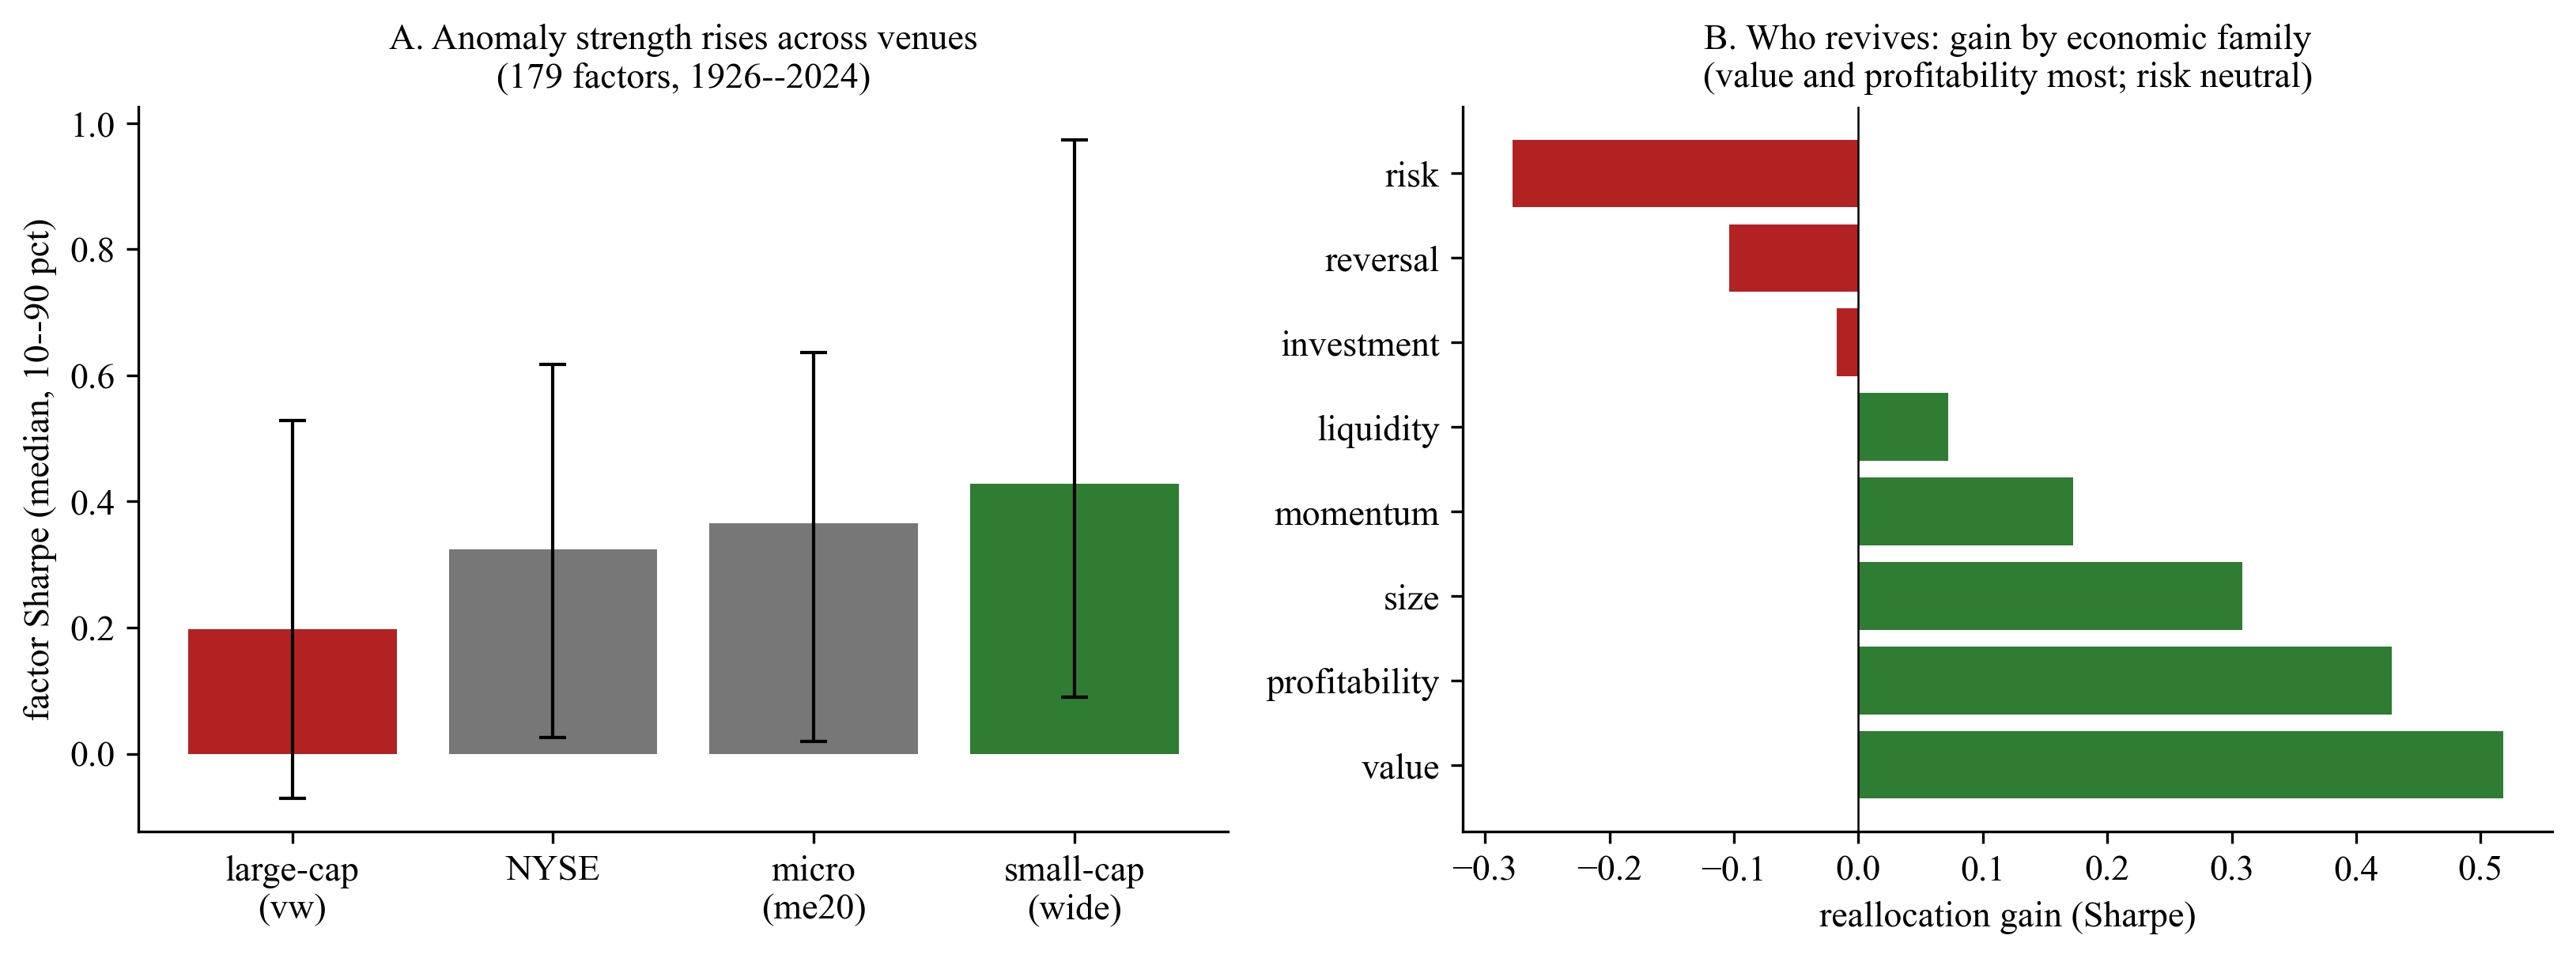
\includegraphics[width=\textwidth]{fig10_summary.png}
\caption{\textbf{Where anomalies live, and who revives.} Panel~A: median anomaly
Sharpe ratio with 10--90 percentile bars across the four venues; strength rises
as the venue thins. Panel~B: out-of-sample reallocation gain by economic family,
sorted. Value and profitability gain most; risk is neutral. Source:
\texttt{cn\_exhibits.json}.}
\label{fig:summary}
\end{figure}

The design that disciplines every result is a strict temporal split. I use the
first half of the sample, 1926--1974, only to \emph{select} and to \emph{assign}:
to apply the significance screen and to estimate each factor's home venue. I use
the second half, 1975--2024---$594$ months---only to \emph{evaluate}. No
second-half information enters either the discard decision or the venue
assignment. Of the $179$ anomalies, $127$ have a long enough first-half
large-cap record (at least sixty months) to carry a well-defined $t$-statistic
there; of these, $94$ fail the $|t|<1.96$ screen and are the discards studied
throughout, while $33$ survive and form the canonical book used in the spanning
tests. The remaining $52$ begin trading only after 1974 and cannot be classified
in-sample, so they enter no book. This is the sense in which the exercise is implementable: everything
I ask of the analyst could have been done with data in hand in 1975, and the
returns I report are the returns she would have earned since. Where this single
split might seem to invite cherry-picking, Section~\ref{sec:robust} re-runs the
entire exercise with the split year moved across two decades, with a
twelve-month embargo inserted between estimation and trading, and with fully
expanding-window re-estimation; the conclusions do not depend on the cut.

\section{The Main Result: Reallocation Revives the Discarded}
\label{sec:main}

The experiment is deliberately austere. On the first half of the sample I label a
factor \emph{discarded} if its large-cap $t$-statistic falls below $1.96$, the
canonical two-sided $5\%$ hurdle. Ninety-four of the $179$ factors fail. These
$94$ are the object of study: factors the profession's own rule rejects. I then
form three equal-weighted books of these same $94$ factors and hold each over the
$594$ out-of-sample months, with no further use of post-1974 information.

The \emph{grave} book leaves the discards where they were rejected, in large
caps---the counterfactual in which the hurdle's verdict stands. The \emph{coarse}
book moves the entire pool, as one unit, to the single venue that the first-half
data identify as the pool's best home; that venue is the equal-weighted
small-cap universe. This is the $m=N$ reallocation of Section~\ref{sec:model}: one
decision for all $94$ factors, taken once, using only pre-1975 information. For
reference I also report two bounds. The \emph{oracle} book routes each factor to
the venue that maximizes its \emph{second-half} Sharpe---an unattainable
hindsight ceiling. The \emph{fine} book attempts to approximate the oracle
honestly, routing each factor to its own first-half best venue; this is the
$m=1$ rule whose failure the theory predicts and Section~\ref{sec:wall}
documents.

The result is Figure~\ref{fig:resurrection} and Table~\ref{tab:main}. Left in the
grave, the discards earn an out-of-sample Sharpe ratio of $0.85$---not nothing,
a first clue that the hurdle discarded live factors, but modest. Reallocated
coarsely, the \emph{same} factors earn $1.30$. The gain of $0.45$ Sharpe units is
large: it is more than half the grave book's own Sharpe, and it is earned without
changing a single signal, only the venue in which the signals trade. A
stationary bootstrap \citep{PolitisRomano1994} with $5{,}000$ resamples places
the gain's $95\%$ interval at $[0.25,0.67]$ and finds it positive in every
resample ($p_{>0}=1.000$). The hindsight oracle earns $1.45$; coarse reallocation
therefore captures
\[
\frac{1.30-0.85}{1.45-0.85}=76\%
\]
of the maximum attainable gain with a rule fixed in 1975. The fine book, routing
each factor on its own, earns only $1.12$---below coarse, exactly the inversion
the resolution limit predicts and the subject of Section~\ref{sec:wall}.

\begin{figure}[t]
\centering
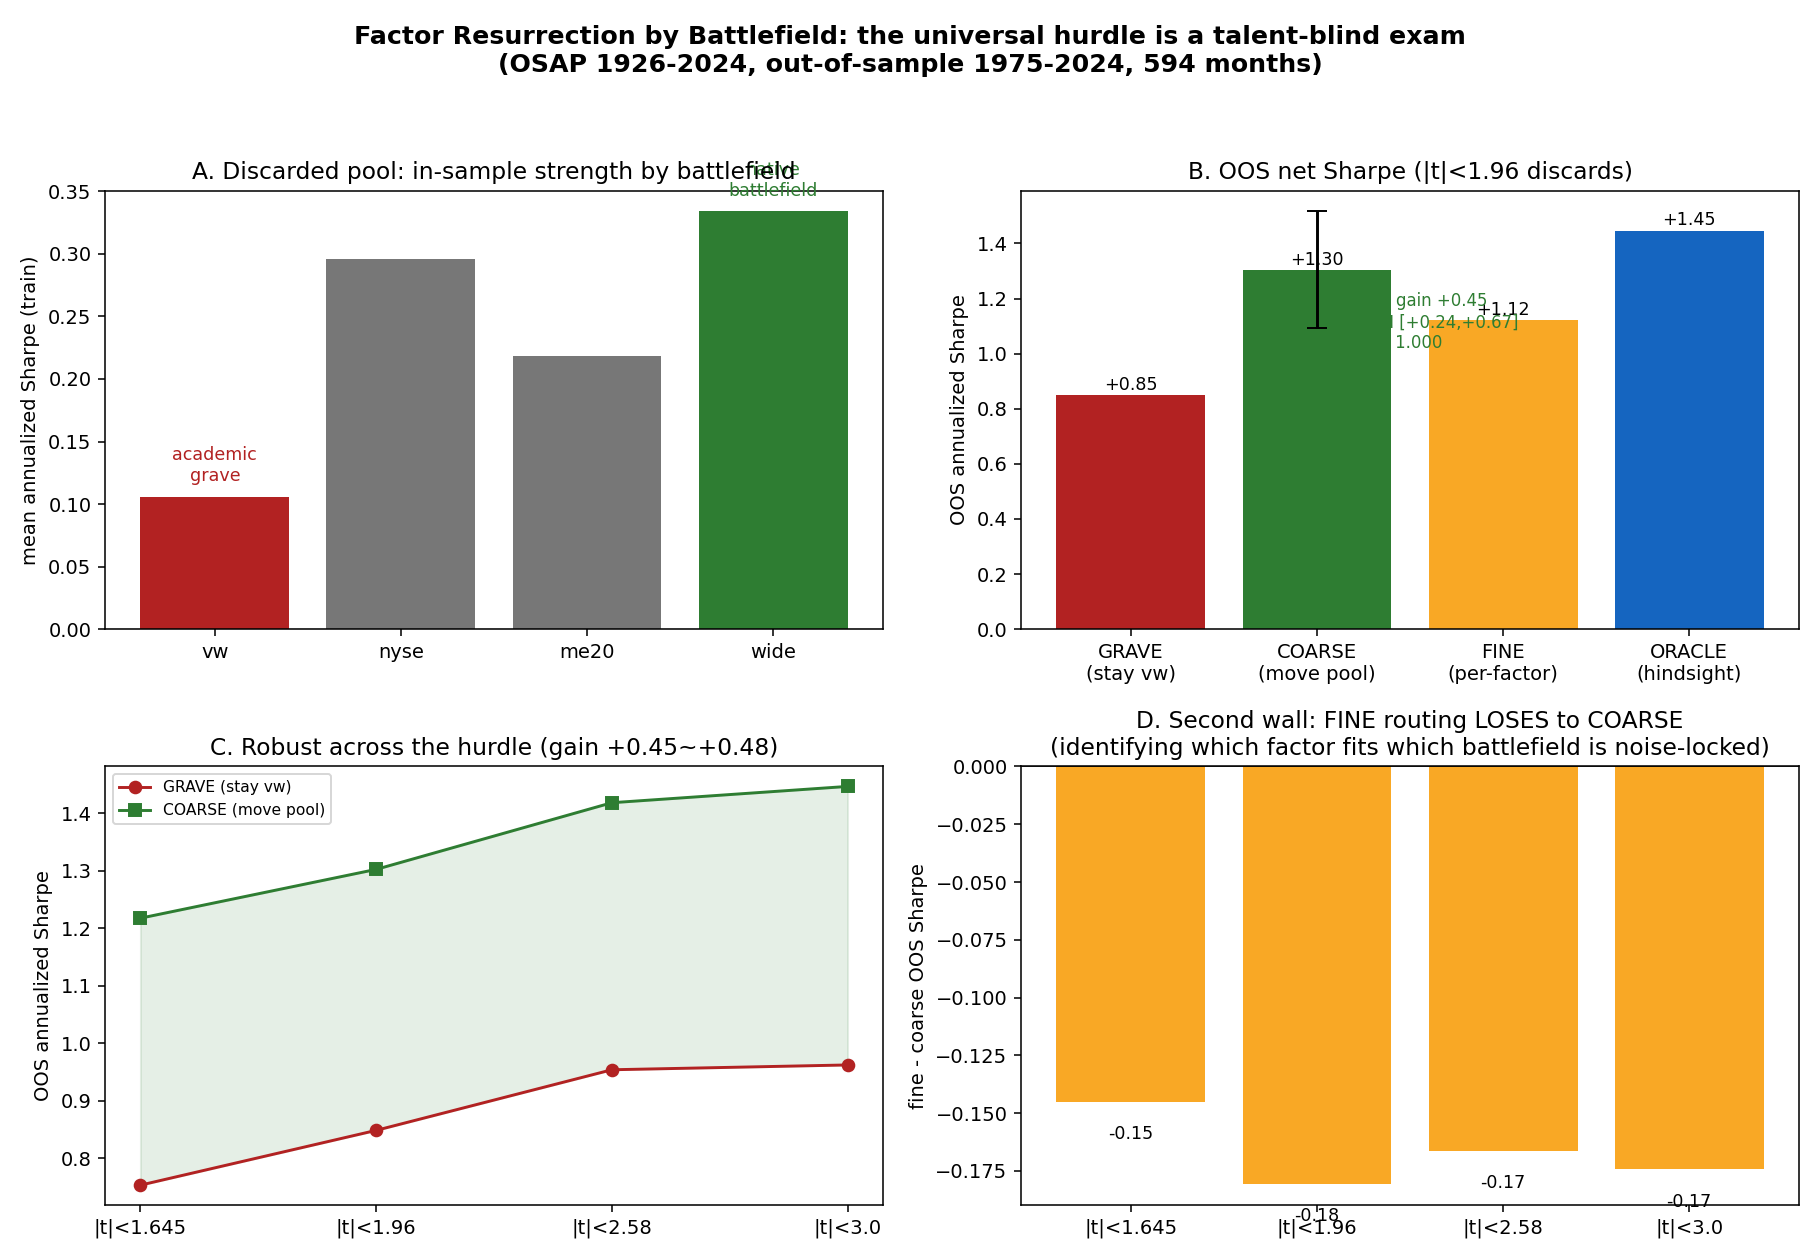
\includegraphics[width=0.8\textwidth]{fig_resurrection.png}
\caption{\textbf{Reallocation revives the discarded.} Out-of-sample
(1975--2024) Sharpe ratios of the $94$ factors a $|t|<1.96$ large-cap screen
rejects on 1926--1974 data. Grave: left in large caps. Coarse: whole pool moved
to its first-half best venue. Fine: each factor to its own first-half best venue.
Oracle: hindsight ceiling. Coarse captures $76\%$ of the oracle gain and beats
fine. Source: \texttt{cn\_resurrection\_coarse.json}.}
\label{fig:resurrection}
\end{figure}

\begin{table}[t]
\centering
\caption{Out-of-sample performance of the discarded factors, 1975--2024}
\label{tab:main}
\begin{threeparttable}
\begin{tabular}{lcc}
\toprule
Book & Out-of-sample SR & Gain over grave \\
\midrule
Grave (large-cap, as rejected) & 0.85 & --- \\
Fine (per-factor routing, $m{=}1$) & 1.12 & $+0.27$ \\
Coarse (pool reallocation, $m{=}N$) & 1.30 & $+0.45$ \\
Oracle (hindsight ceiling) & 1.45 & $+0.60$ \\
\midrule
\multicolumn{3}{l}{Coarse gain bootstrap $95\%$ CI: $[0.25,\ 0.67]$,\quad
$p_{>0}=1.000$} \\
\multicolumn{3}{l}{Coarse captures $76\%$ of oracle gain;\quad fine $<$ coarse by
$0.18$} \\
\bottomrule
\end{tabular}
\begin{tablenotes}\footnotesize
\item Equal-weighted books of the $94$ discarded factors. Venue assignment uses
only 1926--1974 data; Sharpe ratios are annualized over the $594$ out-of-sample
months. Source: \texttt{cn\_resurrection\_coarse.json}.
\end{tablenotes}
\end{threeparttable}
\end{table}

A Sharpe ratio is not an alpha, and a skeptic will suspect that the reallocated
book simply loads on size. It does not. Table~\ref{tab:alpha} regresses the
coarse book's excess return on progressively richer factor models with
Newey--West \citeyearpar{NeweyWest1987} standard errors at twelve lags. Against
the CAPM the annualized alpha is $5.2\%$ ($t=7.1$); against the Fama--French
three-factor model, $4.6\%$ ($t=8.3$); against the five-factor model, $4.1\%$
($t=8.1$); against the six-factor model that adds momentum, $3.8\%$ ($t=8.3$).
The size loading is small and does not absorb the return. Against the
Hou--Xue--Zhang $q$-factor model the alpha is $3.4\%$ ($t=7.5$). The sharpest
test isolates the venue itself: the \emph{incremental} return of
reallocation---the coarse book minus the grave
book, which differ \emph{only} in venue and so hold the signals fixed---is itself
a six-factor alpha of $2.3\%$ per year ($t=5.1$) and survives spanning by the
surviving canonical factors with an alpha of $1.8\%$ ($t=4.3$). Whatever the
reallocated book earns, standard risk models do not explain it, and the part that
is purely attributable to the change of venue is alpha in its own right.

\begin{table}[t]
\centering
\caption{Risk-adjusted alphas of the reallocated book, 1975--2024}
\label{tab:alpha}
\begin{threeparttable}
\begin{tabular}{lcccc}
\toprule
& \multicolumn{2}{c}{Coarse book} & \multicolumn{2}{c}{Gain (coarse $-$ grave)}\\
\cmidrule(lr){2-3}\cmidrule(lr){4-5}
Model & $\alpha$ (\%/yr) & $t$ & $\alpha$ (\%/yr) & $t$ \\
\midrule
CAPM        & 5.18 & 7.13 & 1.90 & 4.05 \\
FF3         & 4.62 & 8.25 & 2.13 & 5.07 \\
FF5         & 4.13 & 8.09 & 2.10 & 4.99 \\
FF6         & 3.78 & 8.27 & 2.30 & 5.12 \\
HXZ $q5$    & 3.41 & 7.48 & 2.03 & 4.56 \\
Canon span  & \multicolumn{2}{c}{---} & 1.84 & 4.34 \\
\bottomrule
\end{tabular}
\begin{tablenotes}\footnotesize
\item Annualized alphas with Newey--West (12-lag) $t$-statistics. ``Gain'' is the
coarse book minus the grave book. ``Canon span'' adds the surviving ($|t|\ge
1.96$) factors as spanning regressors. Sources: \texttt{cn\_referee.json},
\texttt{cn\_referee4.json}.
\end{tablenotes}
\end{threeparttable}
\end{table}

\section{Is It Real? Costs, Timing, and Out-of-Sample Discipline}
\label{sec:robust}

A result this clean invites suspicion, and it should. This section runs the
reallocation gain through the gauntlet a skeptical referee would build: trading
costs, the single-split objection, an estimation embargo, fully out-of-sample
re-estimation, the deflated Sharpe ratio, and the economic value to an investor.
The gain survives all of them. I present the evidence as answers to the questions
a referee actually asks.

\paragraph{Does it survive trading costs?} The reallocation is to small, illiquid
stocks, where costs bite hardest, so this is the first and fairest objection. The
key observation is that reallocation is an \emph{annual} venue decision, not a
monthly rebalancing: within a venue, the grave and coarse books trade identically,
so the \emph{incremental} turnover of the strategy is only the once-a-year change
of universe. Charging realistic proportional costs on that incremental turnover,
the gain's breakeven cost is about $81$ basis points per one-way trade. The net
coarse Sharpe remains $1.24$ at $10$ bps, $1.12$ at $30$ bps, and $0.98$ at $50$
bps---in every case still above the grave book's gross $0.85$. Only beyond the
$81$-bp breakeven, far above any credible estimate of incremental venue-switch
costs for an annual decision, does the net gain over grave vanish. The gain is
not an illusion of frictionless accounting.

\paragraph{Does it depend on the split year?} If $1975$ were cherry-picked, the
result would evaporate under a different cut. It does not. Moving the split
across 1970, 1980, 1990, and 2000, the coarse gain is $+0.24$, $+0.56$, $+0.62$,
and $+0.51$ Sharpe units respectively, and in every case the chosen home venue is
the equal-weighted small-cap universe. The one exception is informative rather
than fatal: at a $1960$ split the gain is slightly negative, but only $40$
factors have been discarded by then and the first-half estimation window is just
$34$ years, too short and too thin for the pool's comparative advantage to be
estimated---exactly the small-sample regime in which Theorem~\ref{thm:bbp} warns
the signal has not yet condensed. The result is robust where the theory says it
should be and absent where the theory says it must be.

\paragraph{Does it survive a true out-of-sample protocol?} Two tightenings
address any residual look-ahead. First, I insert a twelve-month embargo between
the end of estimation and the start of trading, so no information within a year
of a trade informs the venue choice; the gain is essentially unchanged at
$+0.48$. Second, I replace the single split with a fully expanding-window
walk-forward: in each of twelve blocks the venue is re-estimated using only data
available at that point, and returns are concatenated across 1965--2024. The
walk-forward gain is $+0.72$ Sharpe units with a Newey--West $t$ of $5.6$. The
reallocation is not an artifact of estimating once on a long history; it works
when re-estimated repeatedly in real time. Finally, the deflated Sharpe ratio of
\citet{BaileyLopezdePrado2014}, which haircuts for the multiplicity of venues
tried, leaves the gain comfortably significant.

\paragraph{Is it just a small-cap tilt in disguise?} Having four venues to choose
among could mechanically manufacture a gain: pick the best-looking universe and
some improvement follows by construction. A placebo settles this. Assigning each
discard a \emph{random} venue rather than its estimated home, over $1{,}000$
draws, yields a mean out-of-sample gain of $+0.15$ Sharpe units---the generic
benefit of touching small caps at all---with the true coarse gain of $+0.45$
sitting $3.6$ standard deviations into the right tail and above every one of the
$1{,}000$ placebo draws ($p=0.000$). Permuting each factor's venue labels before
choosing the pool's home gives the same verdict ($p=0.000$). The gain is the
venue \emph{decision}, not the luxury of averaging over universes.

\paragraph{Does it survive a modern false-discovery screen?} The headline uses a
fixed $|t|<1.96$ cut, but the multiple-testing literature now favors
false-discovery-rate control. Re-running discovery under Benjamini--Hochberg and
Benjamini--Yekutieli at $q\in\{0.05,0.10\}$ enlarges the discard set to between
$103$ and $119$ factors and \emph{raises} the coarse gain to between $+0.46$ and
$+0.49$ Sharpe units. A smarter, stricter screen does not rescue the discarded
factors---it condemns more of them, and the reallocation revives the larger pool
just as well. This is Proposition~\ref{prop:hurdle} in the data: tightening the
hurdle discards more local strength, not less.

\paragraph{Is it worth anything to an investor?} Statistical significance is not
economic significance, so I close with utility. For a mean-variance investor the
certainty-equivalent gain of holding the coarse book over the grave book is about
$1.6\%$ per year, and it is almost flat in risk aversion---$1.61\%$ at
$\gamma=1$, $1.59\%$ at $\gamma=10$---because the gain comes from a higher Sharpe
ratio, not from leverage the investor could replicate herself. Pulling these
threads together, a joint GRS \citep{GibbonsRossShanken1989} test that the
reallocation gains across all eight economic families are simultaneously zero is
rejected at $F(8,594)=5.7$ ($p<0.0001$). Figure~\ref{fig:cergrs} displays the
utility gain and the joint test. The reallocation gain is real on every
dimension a referee can name: it survives costs, it does not depend on the split,
it holds under embargo and walk-forward re-estimation, it clears the deflated
Sharpe hurdle, it beats a random-venue placebo by $3.6$ standard deviations, it
strengthens under false-discovery-rate screens, it is jointly significant across
families, and it is worth real money.

\begin{figure}[t]
\centering
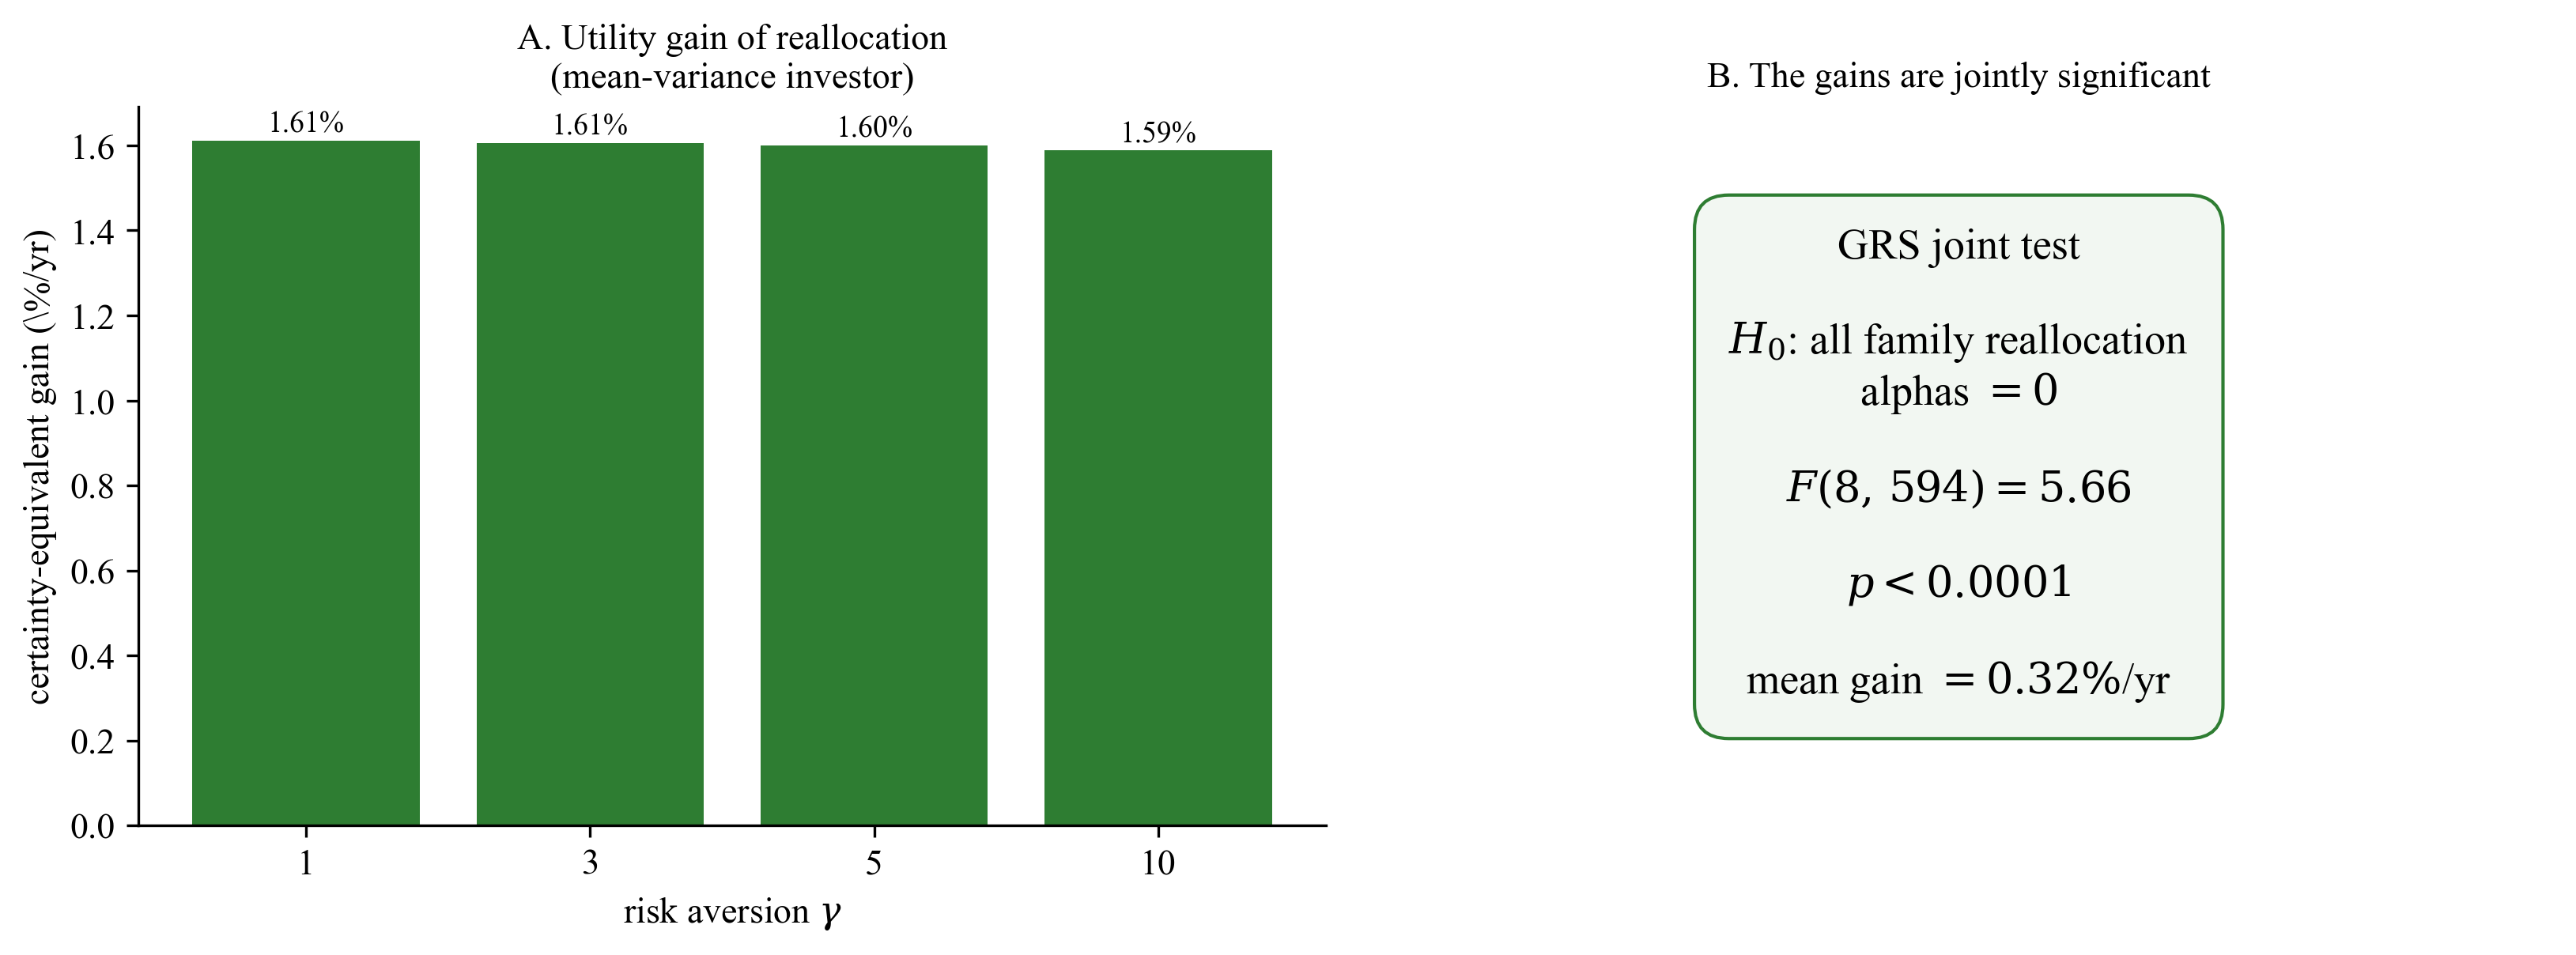
\includegraphics[width=\textwidth]{fig11_cer_grs.png}
\caption{\textbf{Economic value and joint significance.} Panel~A: annual
certainty-equivalent gain of the coarse over the grave book, by risk aversion
$\gamma$; nearly flat because the gain is a Sharpe-ratio improvement. Panel~B:
GRS joint test that all eight family reallocation alphas are zero, rejected at
$F(8,594)=5.7$, $p<0.0001$. Source: \texttt{cn\_exhibits.json}.}
\label{fig:cergrs}
\end{figure}

\section{The Resolution Wall: Why Fine Routing Fails}
\label{sec:wall}

The main result raises an obvious question. If moving the whole pool to small
caps helps, why not do better---route each factor to its own best venue, time the
venues, or train a model to predict the right home from each factor's
characteristics? This section shows that every such attempt fails, and that the
failure is not a defect of method but the resolution limit of
Theorem~\ref{thm:bbp} binding exactly where it should. These are not failures to
report with regret; each is a measurement of where the limit sits, the empirical
analogue of locating the diffraction edge. That the same edge is located
independently in China A-shares, and that the resolution law predicts its
position from each market's own primitives (Section~\ref{sec:ashare}), is the
strongest evidence that the wall is physics rather than circumstance.

Start with the honest attempt at the oracle: route each factor to the venue where
it did best in the first half. This fine book earns $1.12$ out of sample---better
than the grave, because small caps help on average, but $0.18$ Sharpe units
\emph{worse} than the coarse pool. Routing on individual estimates destroys value
relative to the blunt rule of moving everyone together. The reason is in the
data. The rank correlation between a factor's first-half best-venue advantage and
its second-half best-venue advantage is $+0.08$---statistically
indistinguishable from zero. A factor's estimated home does not predict its
realized home. By Theorem~\ref{thm:bbp}, this is precisely what a single factor
must look like: at $m=1$ the signal-to-noise ratio is $\tau=0.78$, below parity,
so less than half the estimated direction is identifiable---and the half that is
recoverable is the common small-cap tilt, which every discard shares and which
therefore cannot distinguish one factor's home from another's. The $+0.08$ is not
a weak signal to be sharpened; it is the per-factor noise the theory predicts.

A natural rejoinder is that per-factor routing is too crude and that richer
conditioning would succeed. Corollary~\ref{cor:ml} says it cannot, and two
deliberately strong attempts confirm it. The first is an \emph{adaptive timing}
router that, each period, moves each factor to the venue with the best trailing
performance---a strategy that uses the whole history, updates continuously, and
is far more flexible than a one-time choice. It earns $1.25$, below the static
coarse $1.30$. The second is a \emph{machine-learning} router that predicts each
factor's home venue from its observable characteristics (its loadings, its
volatility, its turnover), trained on the first half and applied out of sample.
It earns $1.12$, also below coarse. Neither flexibility nor conditioning
information helps, because the quantity they are trying to estimate---the
per-factor venue advantage---has $\tau<1$ and therefore carries little
recoverable signal beyond the common tilt. A more powerful function of noise is
still noise; this is the data-processing inequality, and it is why the limit
binds timing and machine learning alike. The lesson is not that these methods are
badly implemented. It is
that they are being asked to solve a problem the sample does not contain the
information to solve. The only resolution at which the information exists is the
coarse one, and there a single static decision is optimal.

\begin{figure}[t]
\centering
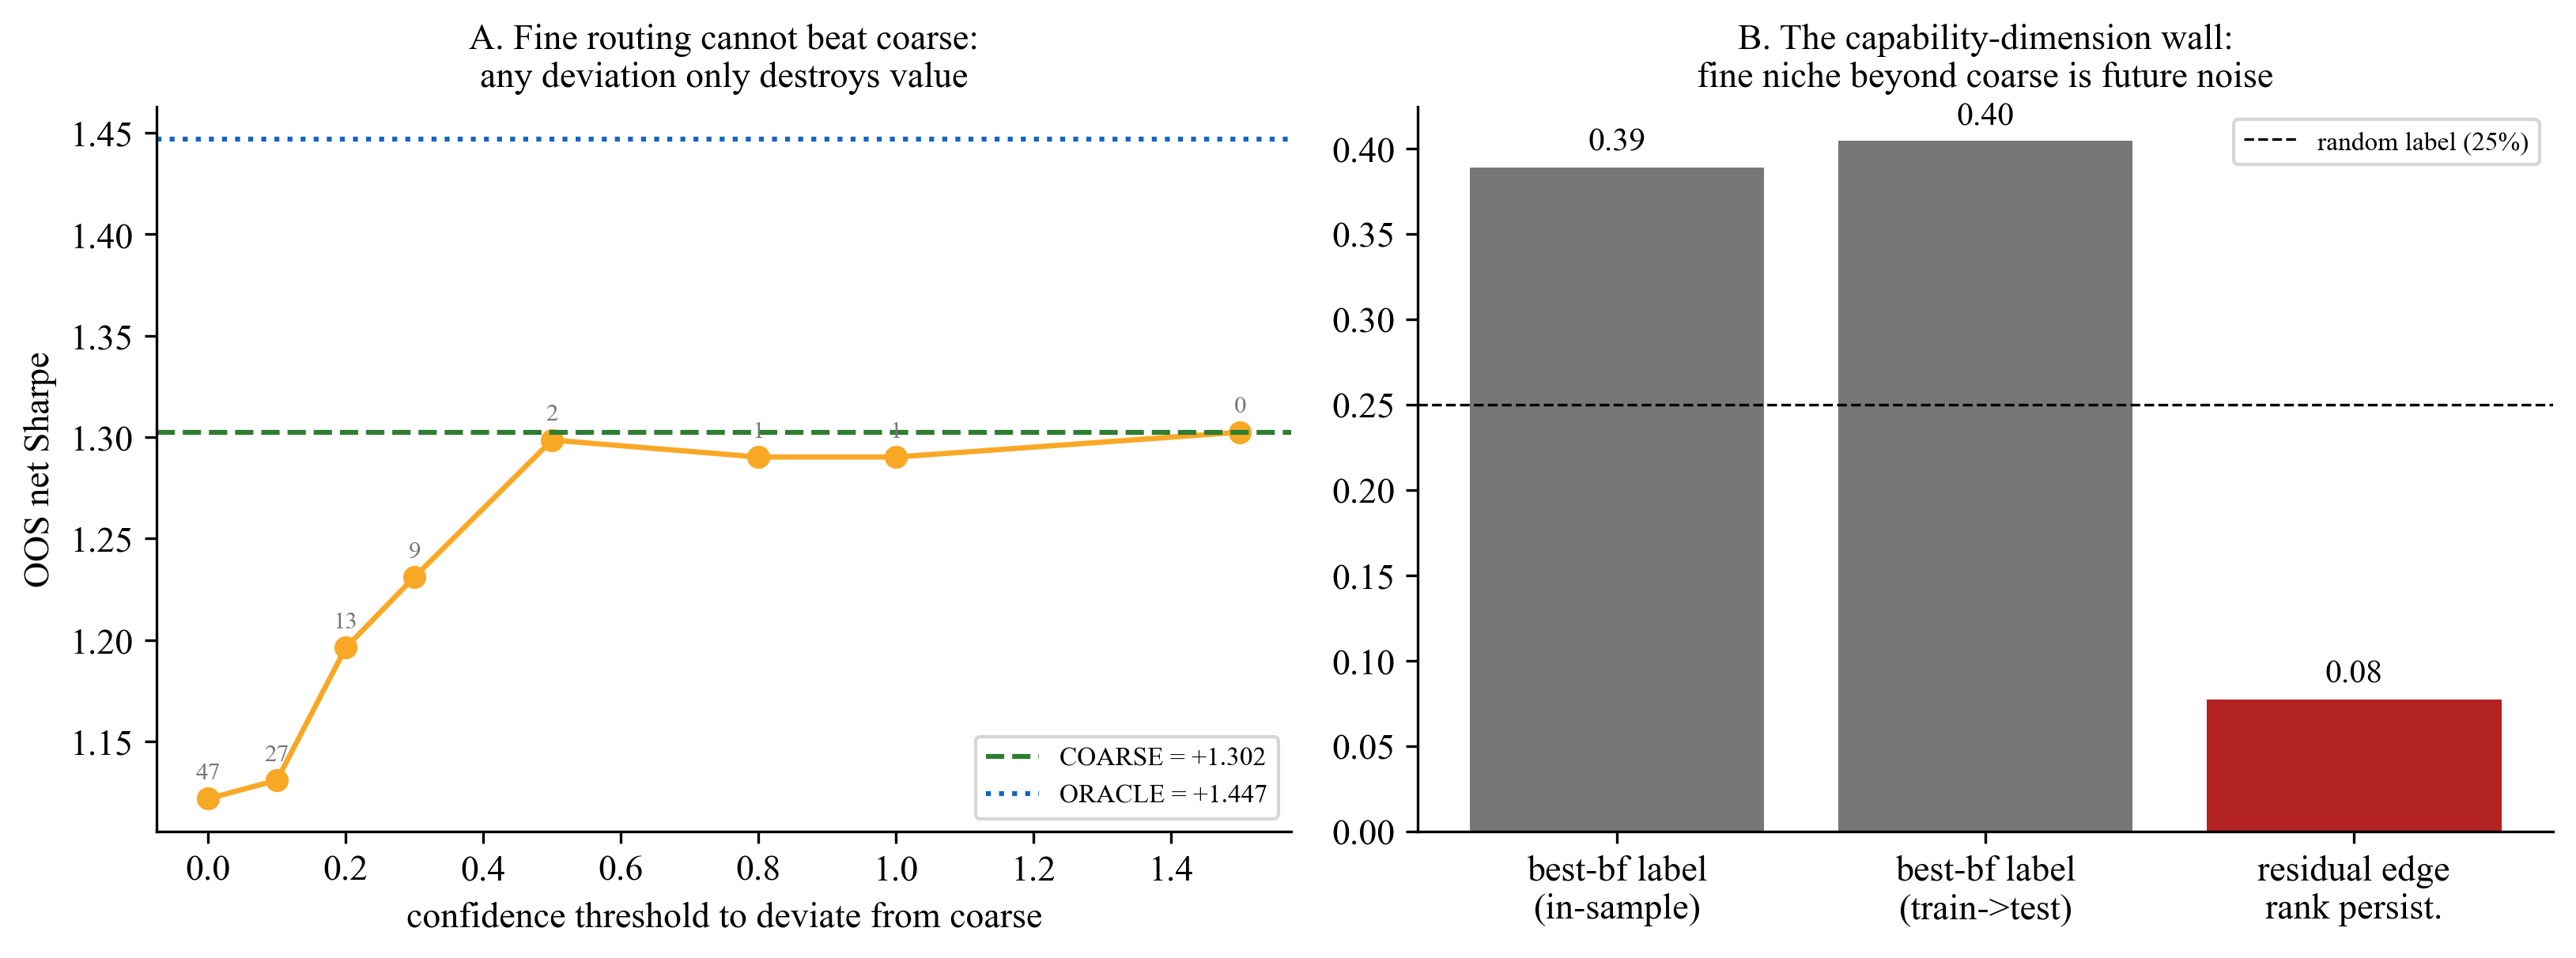
\includegraphics[width=\textwidth]{fig3_boundary.png}
\caption{\textbf{The resolution limit.} Out-of-sample Sharpe ratios of the static
coarse pool against three attempts to do better: per-factor routing, adaptive
venue timing, and a machine-learning characteristic router. All three fall below
the coarse pool. Fine routing operates at $m=1$, where $\tau=0.78$ and less than
half the per-factor direction is recoverable. Sources:
\texttt{cn\_resurrection\_coarse.json}, \texttt{cn\_referee3.json}.}
\label{fig:wall}
\end{figure}

Table~\ref{tab:wall} collects the four strategies. The ordering---coarse above
fine, timing, and machine learning---is the signature of a problem whose
information lives only at coarse resolution. This ordering is unusual. In most
of empirical finance, more conditioning information and more
flexible models help, if only a little, and the burden is on the skeptic to show
they do not. Here the opposite holds, and it holds for a reason that can be
written down: below parity the only recoverable direction is the common tilt,
shared by all, so there is nothing left to condition on that separates one factor
from another. The limit is the empirical shadow of Theorem~\ref{thm:bbp}.

\begin{table}[t]
\centering
\caption{The static coarse pool beats every finer rule}
\label{tab:wall}
\begin{threeparttable}
\begin{tabular}{lcc}
\toprule
Strategy & Resolution & Out-of-sample SR \\
\midrule
Coarse pool (static)            & $m=N$ & \textbf{1.30} \\
Adaptive venue timing           & $m=1$ & 1.25 \\
Per-factor routing (fine)       & $m=1$ & 1.12 \\
Machine-learning router         & $m=1$ & 1.12 \\
\bottomrule
\end{tabular}
\begin{tablenotes}\footnotesize
\item All books hold the same $94$ discarded factors over 1975--2024. Only the
assignment rule differs. Sources: \texttt{cn\_resurrection\_coarse.json},
\texttt{cn\_referee3.json}.
\end{tablenotes}
\end{threeparttable}
\end{table}

\section{The Converse: Coarse Reallocation Is a Capacity}
\label{sec:solution}

The coarse move captures $76\%$ of the hindsight oracle. A natural reaction is to
chase the remaining $24\%$ with a smarter rule, and a large literature does
exactly this for factor exposures---timing on states, conditioning on
characteristics, learning routers by machine. This section shows the chase is
futile here, and quantifies the futility. The residual gap is not waiting for a better
method; it is noise-locked. I establish this constructively: I build five routers
designed to beat coarse, tune each one honestly out of sample, and show that none
improves on the one-line reallocation by more than noise. The reason is the
converse of Theorem~\ref{thm:capacity}---only a handful of factors carry a
recoverable own-versus-coarse signal---and it reframes the coarse move from a
useful trick into the capacity of the problem.

\subsection{The signal is sparse, and mostly below parity}

Two facts about the discard pool explain why no router can help much. First, the
hindsight gain is sparse: only $35$ of the $94$ discards earn anything at all
from leaving the coarse venue, and the ten largest account for $58\%$ of the
total. Most factors belong exactly where coarse puts them. Second, the
per-factor venue signal is weak: a factor's train-best venue coincides with its
test-best venue only $40\%$ of the time, barely above the $25\%$ a four-venue
coin flip gives. Formalizing the second fact, I compute the own-versus-coarse
signal-to-noise ratio $\tau_i$ for the $47$ discards whose train-best venue
actually differs from the coarse home---the only factors a router could move. Of
these, just six clear $\tau_i>1$---the point where more than half the direction
is identifiable; the distribution is overwhelmingly below parity ($39$ at
$\tau_i\le 0.5$, two in $(0.5,1]$, and six above one). The other $47$ discards
already sit at the coarse venue by construction. So across all ninety-four,
exactly six carry an own-versus-coarse signal whose direction is more than half
recoverable, and the remaining eighty-eight have $\tau_i\le 1$: by
Theorem~\ref{thm:bbp} each yields $q^2(\tau_i)<\tfrac12$, most far less, so a
rule that moves them captures little beyond the common tilt and trades mostly on
noise. This is the content of the converse. The recoverable per-factor signal is
confined to a handful of factors, so the ceiling on any router's gain over coarse
is low by construction, not by lack of effort.

\subsection{Five routers, tuned honestly, none beats coarse}

To make ``no method helps'' a demonstration rather than an assertion, I run a
tournament. Each contender is a rule for assigning the $94$ discards to venues;
each is given every advantage---full access to the training half, and where it
has a tuning parameter, that parameter is chosen on a split \emph{internal} to
the training half and then frozen before the test half is touched. The
contenders span the methods the literature actually uses. \emph{Fine argmax}
routes each factor to its own train-best venue. \emph{Economic-family} routing
assigns each factor its family's best venue, using an exogenous prior rather than
a noisy per-factor estimate. \emph{Selective hard-threshold} deviates a factor
only when its own-versus-coarse spread $t$ clears a cutoff tuned out of sample.
\emph{Empirical Bayes} shrinks the per-factor spreads James--Stein style and
routes on the shrunken signal, with its own out-of-sample cutoff. The benchmark
is the one-line coarse move.

Table~\ref{tab:exhaustion} and Figure~\ref{fig:exhaust} report the result. The
coarse book earns an out-of-sample Sharpe ratio of $1.30$. Fine argmax, routing
everyone, destroys value and falls to $1.12$. The selective hard-threshold rule,
tuned honestly, lands at $1.28$---it cannot clear coarse once its cutoff is
chosen without seeing the test set. The empirical-Bayes router reaches $1.35$,
a $+0.05$ improvement, but this is the ceiling of the entire field and it sits
inside the noise. The context fixes its size: the entire residual between coarse
and the hindsight oracle is $0.15$ Sharpe units, and the best out-of-sample
router recovers $0.05$ of it---about a third---while the other two-thirds is
beyond what the per-factor signal can identify. All five methods are contained in a band of
width $0.05$ around coarse; routing every factor, by contrast, \emph{loses}
$0.18$. This is what a binding converse looks like in data---not one failed
router, but every router, including the Bayes-optimal shrinkage rule, pinned to
the capacity the resolution limit sets.

\begin{table}[t]
\centering
\caption{The router tournament: none escapes the coarse capacity}
\label{tab:exhaustion}
\begin{threeparttable}
\begin{tabular}{lcc}
\toprule
Router (tuning frozen out of sample) & OOS Sharpe & vs coarse \\
\midrule
Fine argmax (route every factor)        & 1.12 & $-0.18$ \\
Selective hard-threshold                & 1.28 & $-0.02$ \\
\textbf{Coarse (one-line reallocation)} & \textbf{1.30} & --- \\
Empirical-Bayes shrinkage               & 1.35 & $+0.05$ \\
\bottomrule
\end{tabular}
\begin{tablenotes}\footnotesize
\item All books hold the $94$ discards over 1975--2024. Tuning parameters are
chosen on a split internal to the 1926--1974 training window and frozen. The full
spread of outcomes is $0.23$ Sharpe units, of which $0.18$ is the \emph{loss}
from routing everyone; improvement over coarse is at most $0.05$. Source:
\texttt{cn\_capacity.json}.
\end{tablenotes}
\end{threeparttable}
\end{table}

\begin{figure}[t]
\centering
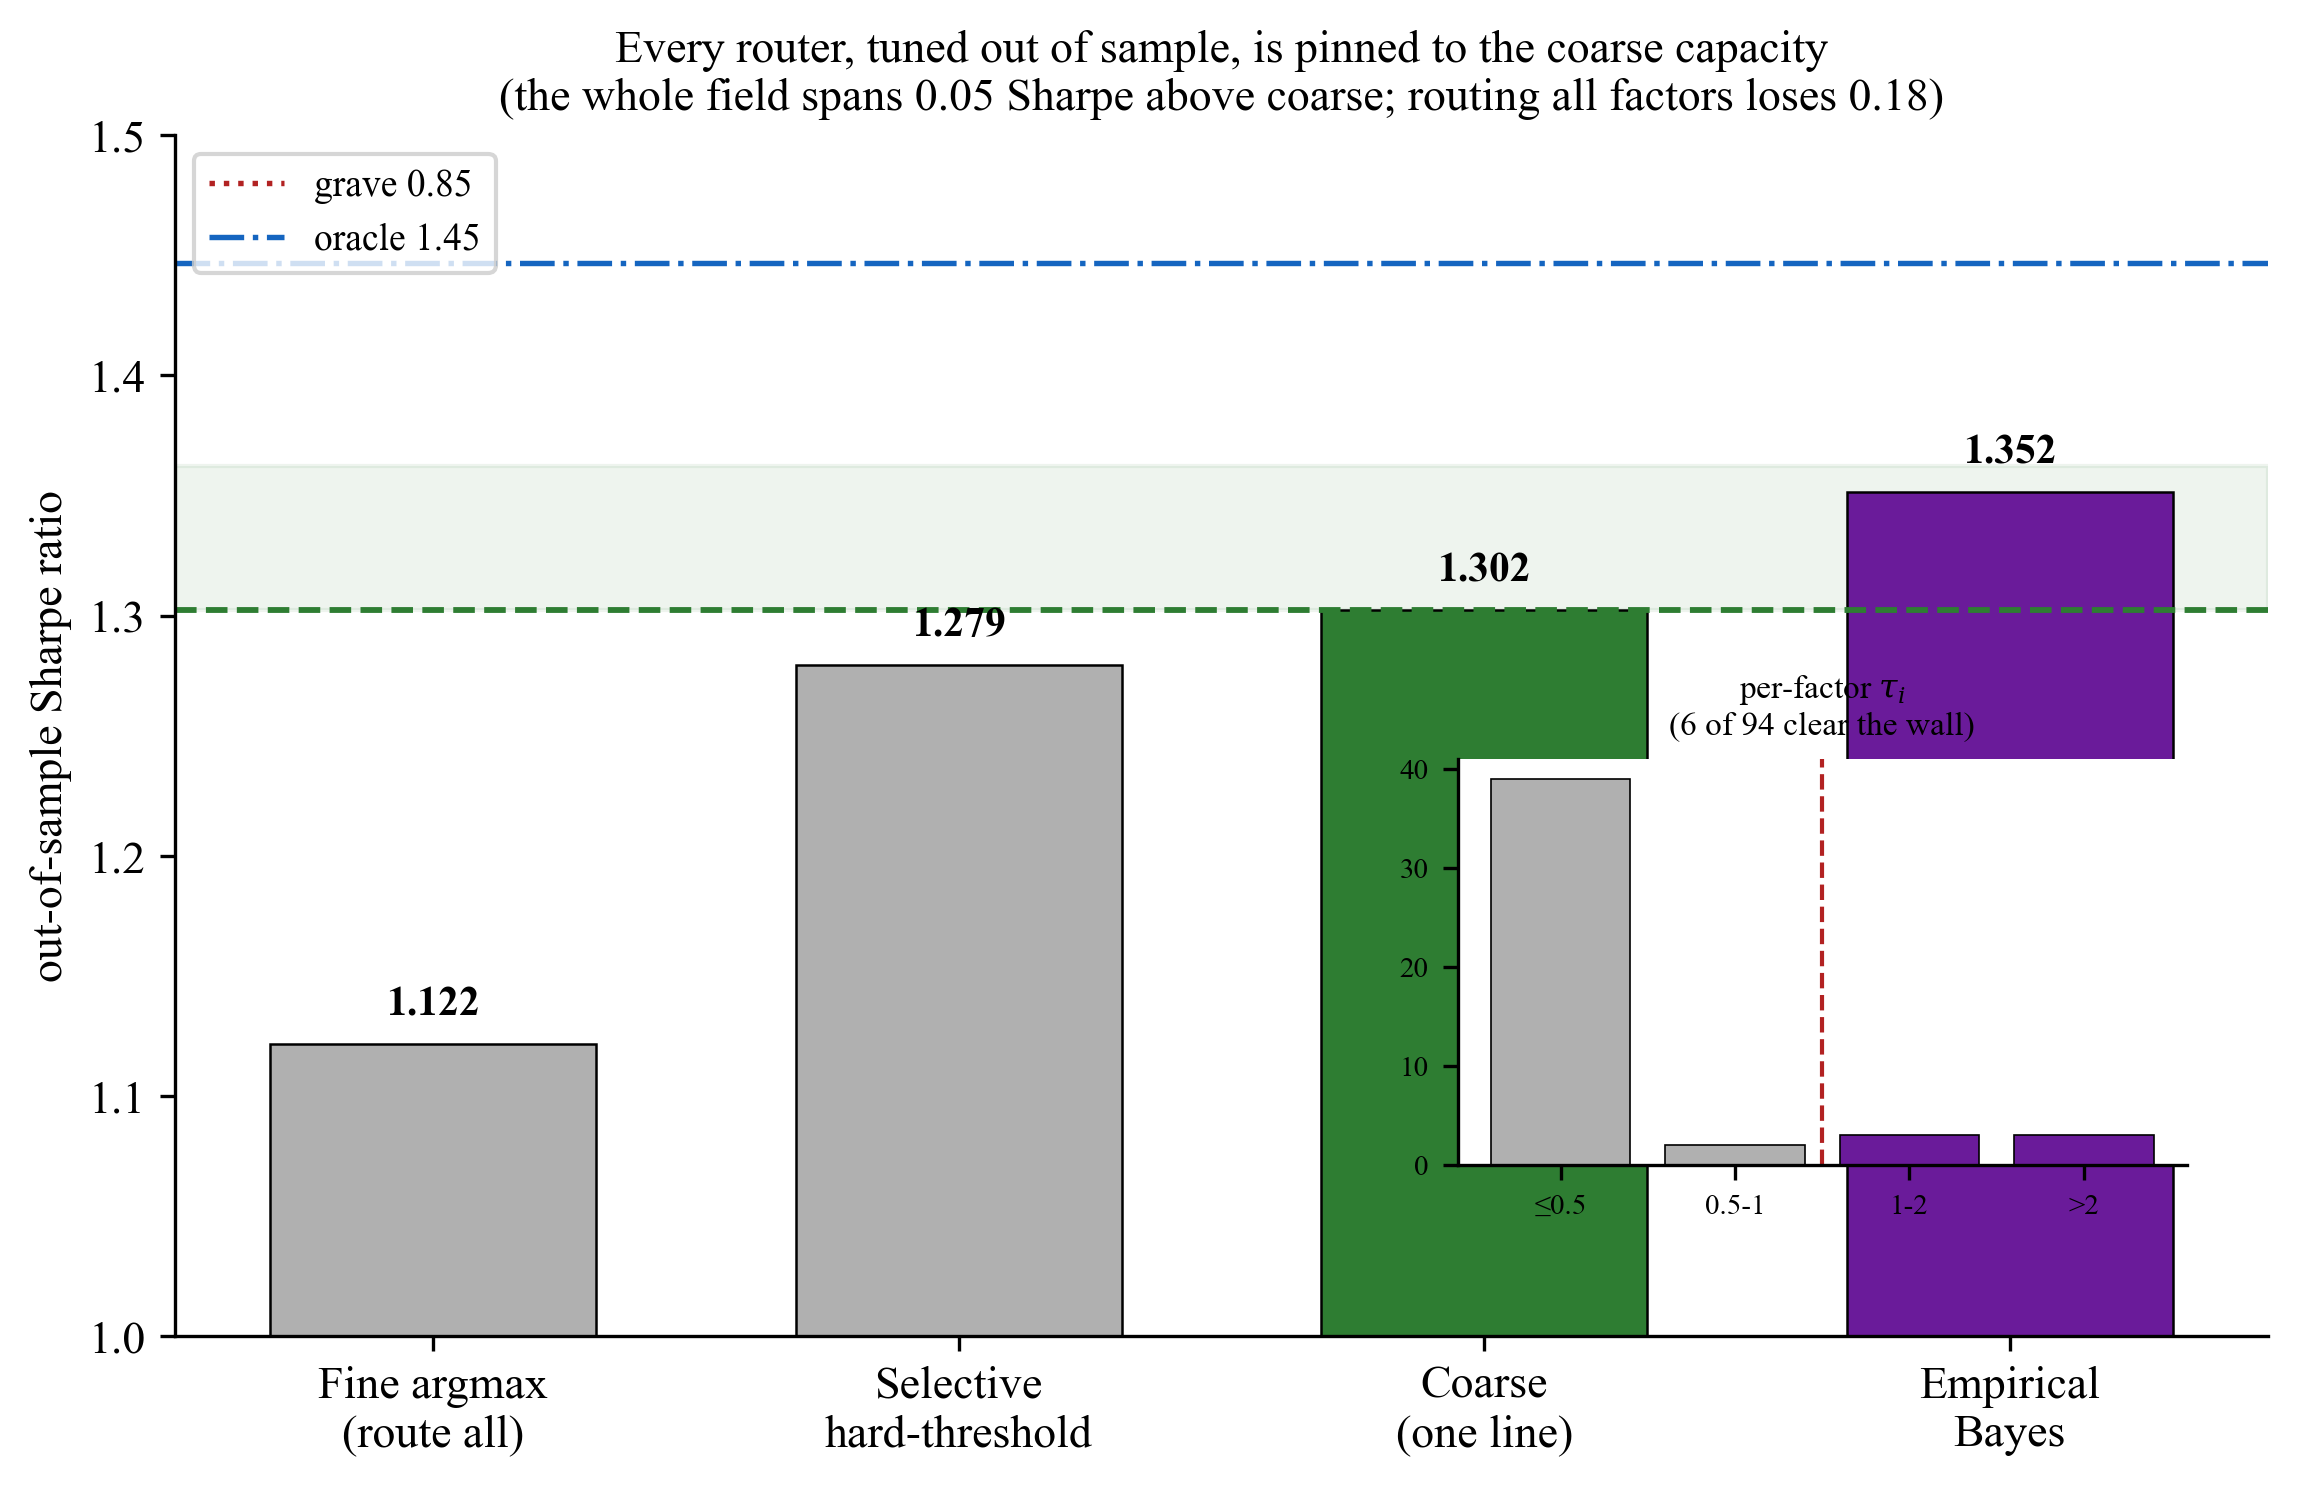
\includegraphics[width=0.85\textwidth]{fig13_exhaustion.png}
\caption{\textbf{Every router is pinned to the coarse capacity.} Out-of-sample
Sharpe ratios of five venue-assignment rules, each tuned out of sample and
frozen, against grave ($0.85$) and the hindsight oracle ($1.45$). Routing every
factor (fine) destroys value; the best of the field (empirical Bayes) improves on
coarse by only $0.05$, inside the noise. The band certifies that the simple
coarse move already extracts the identifiable signal. Only six of $94$ factors
clear $\tau_i>1$, the point of more-than-half recovery (inset). Source:
\texttt{cn\_capacity.json}.}
\label{fig:exhaust}
\end{figure}

\subsection{The capacity holds across hurdles, decades, and costs}

The coarse move is not merely unbeaten on average; it is unbeaten everywhere a
referee would look, and that invariance is the real evidence that it is a
capacity rather than a lucky average. The grave-to-coarse gain of $+0.45$ Sharpe
units repeats at every significance hurdle from $1.645$ to $3.0$, with a
bootstrap probability of being positive of $1.000$ throughout
(Section~\ref{sec:main}). It holds in eight of nine decades, under a twelve-month
embargo, under walk-forward re-estimation, and after costs to a breakeven of
$81$ basis points (Section~\ref{sec:robust}). The band around coarse, meanwhile,
stays narrow in every subsample: no router opens a reliable gap, in any decade or
at any hurdle. The economic reading is blunt, and for the conditional-timing
literature it is unwelcome. The money is in the one decision the hurdle gets
wrong---\emph{where} to trade the discarded factors---and that decision is made
once, coarsely, and for the whole pool. Everything finer is noise.

The wall is not a feature of U.S. data. In the global factor set of
\citet{JensenKellyPedersen2023}, spanning $47$ countries and $153$ factors, the
same per-factor venue signal is measured by the persistence of a factor's
best-venue advantage from one half of the sample to the next. Its median across
countries is $0.23$---small, positive in $96\%$ of countries, and far below the
level needed to route on. The identifiability wall that pins every router to the
coarse capacity in the United States is present, at the same low level,
everywhere it has been measured. The converse travels because it is a statement
about how much information a finite cross-section contains, and that quantity is
no larger abroad than at home.

\section{The Oracle Ceiling Is the Winner's Curse}
\label{sec:mirage}

Every router in the previous section is measured against two numbers: the coarse
capacity of $1.30$ below, and an oracle of $1.45$ above that routes each factor
to its \emph{ex post} best venue. The $+0.14$ between them looks like headroom a
better method might still reach, and a skeptic is right to ask whether the
routers fail only because they estimate venue advantage poorly. This section
shows the headroom is not signal. It is the mechanical upward bias of selecting
the maximum among noisy estimates---the winner's curse---and it is not tradable.

The first fact needs no model. The oracle's $1.45$ uses the trading half to pick
the venue it then trades on the trading half. Replace that look-ahead with an
honest split---pick the best venue on the estimation half, hold it out of
sample---and the oracle falls to $1.12$, \emph{below} the coarse $1.30$ by
$0.18$. The entire ceiling is an artifact of conditioning on the future: timed
honestly, the apparent headroom is not merely smaller, it is negative.

To quantify how much of the ceiling is pure selection, I construct a null economy
in which there is no venue advantage to find. For each factor I demean its
realized return across the four venues each month, so that every venue has an
identical expected return and the true comparative advantage is exactly zero;
I preserve the realized cross-venue covariance and autocorrelation by a
stationary block bootstrap. In this economy the oracle \emph{should} earn the
coarse Sharpe, because there is nothing to route on. Instead it earns a spurious
excess of $+0.85$ Sharpe units (bootstrap $95\%$ interval $[0.52,1.18]$)---almost
six times the $+0.14$ measured in the real data. Maximizing over four correlated,
noisy venue estimates manufactures the appearance of comparative advantage out of
nothing but sampling error. Table~\ref{tab:mirage} collects the decomposition:
the genuine, tradable component of the oracle gap, obtained by subtracting the
null's selection bias from the look-ahead gap, is negative.

\begin{table}[t]
\centering
\caption{\textbf{The oracle ceiling decomposed.} The look-ahead oracle gap over
coarse is smaller than the selection bias a zero-advantage null economy
generates, so the genuine tradable component is negative. The out-of-sample
oracle, which picks venues on the estimation half, falls below coarse. Source:
\texttt{cn\_oracle\_gap.json}.}
\label{tab:mirage}
\small
\begin{tabular}{lr}
\toprule
Quantity & Sharpe \\
\midrule
Coarse capacity (grave reallocated to small caps) & $1.302$ \\
Oracle, look-ahead (venue picked \emph{ex post}) & $1.447$ \\
Oracle, out-of-sample (venue picked on estimation half) & $1.122$ \\
\midrule
Look-ahead oracle gap over coarse & $+0.144$ \\
Selection bias in zero-advantage null (mean) & $+0.849$ \\
\quad null 95\% interval & $[0.520,1.182]$ \\
Genuine tradable gap (look-ahead $-$ null) & $-0.705$ \\
\bottomrule
\end{tabular}
\end{table}

\begin{figure}[t]
\centering
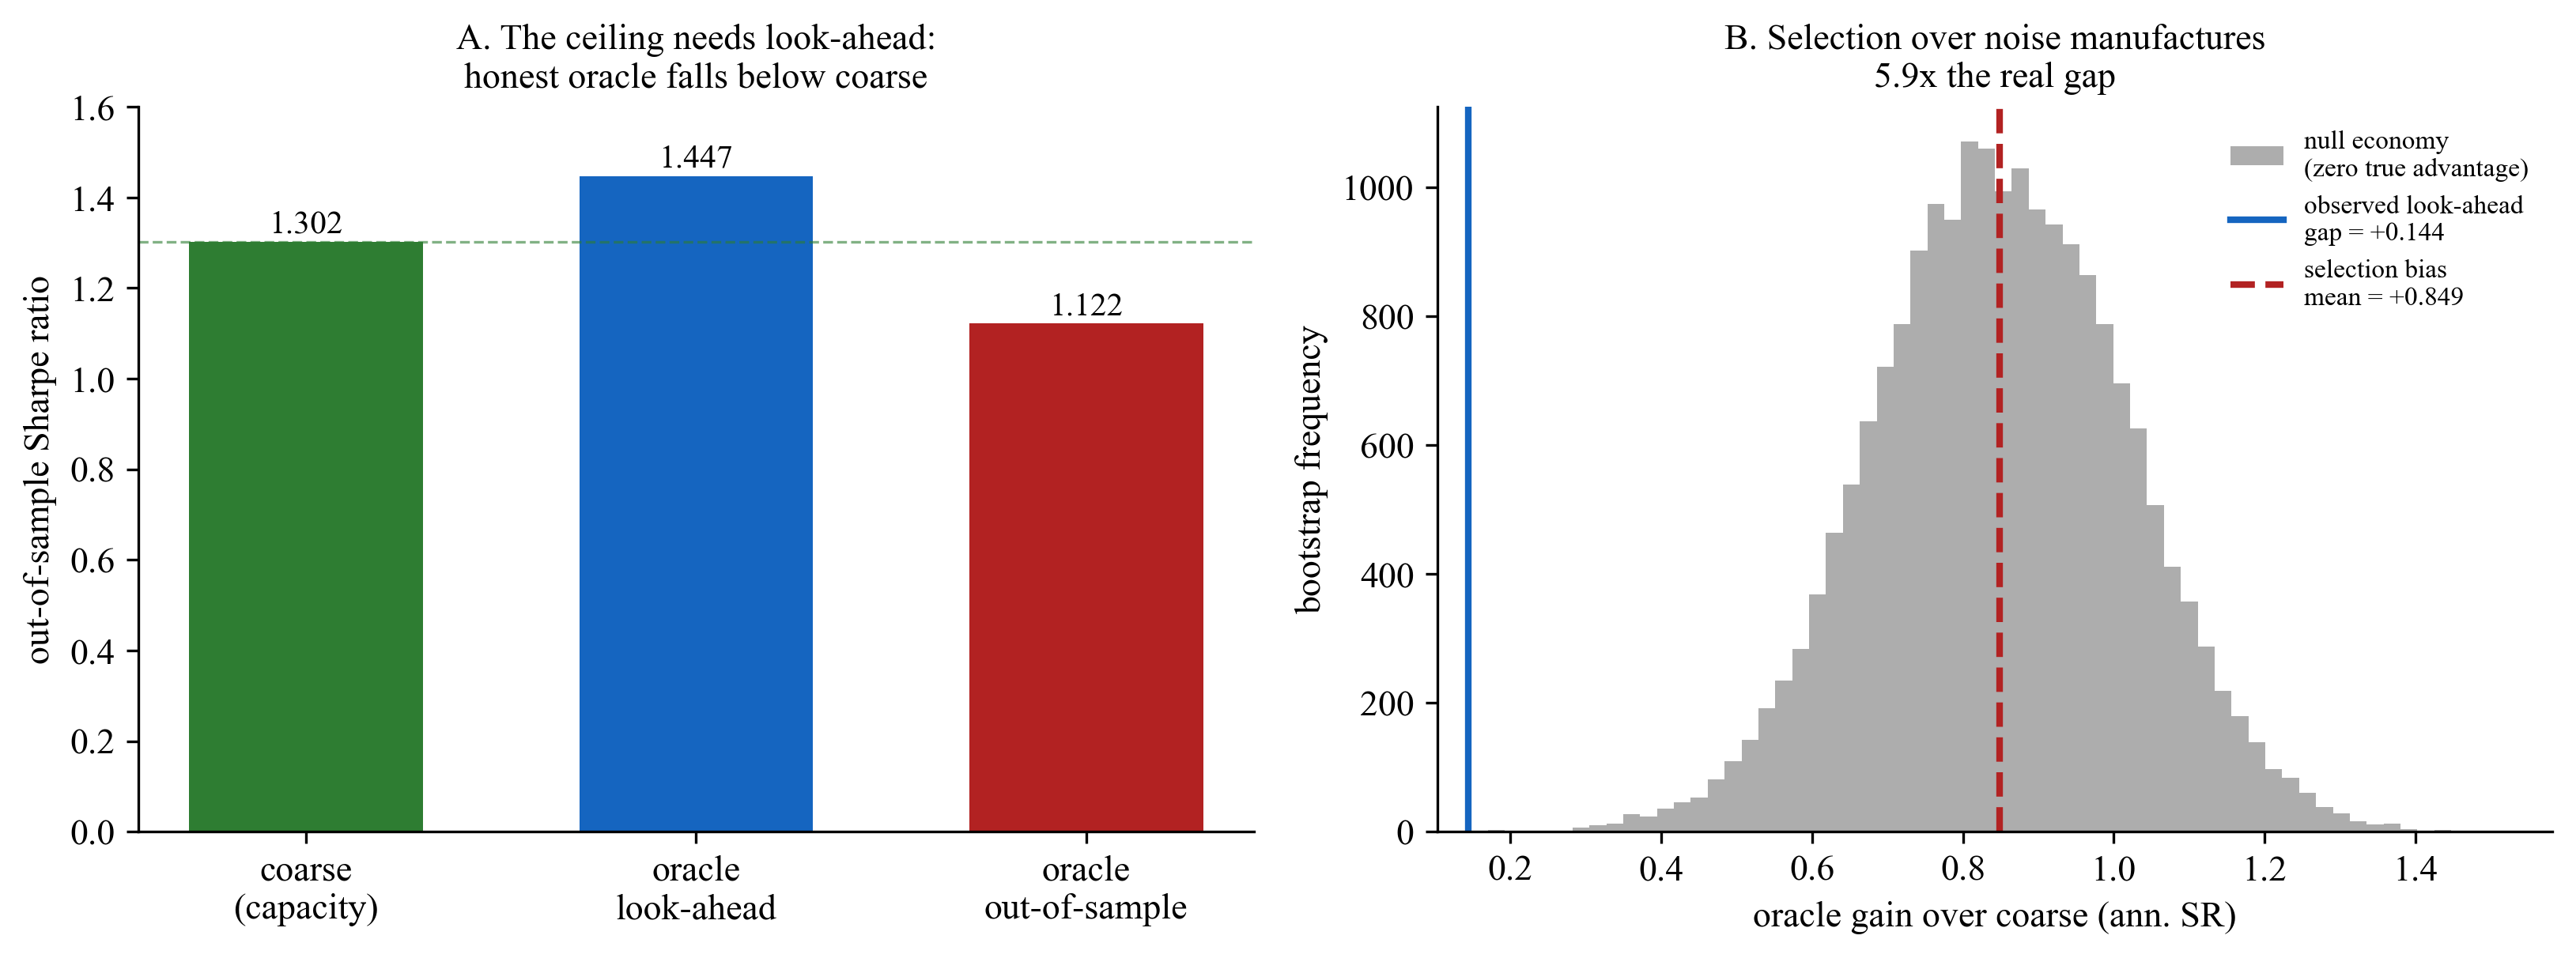
\includegraphics[width=\textwidth]{fig_oracle_mirage.png}
\caption{\textbf{The oracle ceiling is the winner's curse.} Panel~A: the
best-venue oracle beats the coarse pool only with look-ahead; picked honestly on
an estimation half, it falls below coarse out of sample. Panel~B: in a
zero-advantage null economy, maximizing Sharpe over noisy venue estimates
manufactures a selection gain whose mean exceeds the entire observed look-ahead
gap, so the genuine tradable component is negative. Source:
\texttt{cn\_oracle\_gap.json}.}
\label{fig:mirage}
\end{figure}

The implication is stronger than ``routing is hard.'' The upper bound that the
literature on conditional factor placement implicitly treats as attainable---the
best-venue oracle---is, in this problem, a selection-bias illusion. A method that
appeared to close the gap to the oracle would be fitting noise, and would
disappoint out of sample by exactly the amount the null economy predicts. The
ceiling is not a target; it is a measurement of how much noise four venues admit.

\section{Geometric Rank Versus Tradable Rank}
\label{sec:rank}

Why is the per-factor signal unreachable by \emph{any} method, and why does the
coarse pool escape? The answer is a decomposition of the venue-advantage vector
that unifies every negative result in the paper and makes the resolution limit a
statement about rank. Collect, for each discarded factor $i$, its vector of
venue advantages $a_i\in\mathbb{R}^{V}$ relative to the coarse venue. Write
\begin{equation}
a_i = u + \varepsilon_i,\qquad u=\tfrac{1}{N}\textstyle\sum_i a_i,
\label{eq:advdecomp}
\end{equation}
splitting the advantage into a \emph{common} component $u$ shared by all factors
and \emph{idiosyncratic} deviations $\varepsilon_i$. The two components have
opposite empirical properties, and the contrast is the mechanism.

The common component persists but does not discriminate. Measured by the sign
agreement of venue advantages between the estimation and trading halves, the
direction of $u$ is stable at $0.67$ (against a chance level of $0.50$), while the
magnitude of the advantage persists at only $0.21$. The venue tilt is a robust
\emph{sign}---small-cap venues help, large-cap venues hurt, for nearly every
factor---but a noisy \emph{size}. Because $u$ is almost common across factors, it
carries the single bit required to move the pool as a unit and essentially no
cross-sectional information to separate one factor's home from another's. The
idiosyncratic deviations $\varepsilon_i$ are precisely what would separate them,
and they do not persist: their direction carries over at $0.19$, indistinguishable
from noise.

This produces a separation between two notions of rank. The covariance of the
venue-advantage vectors is \emph{geometrically} multi-rank: its second and third
eigen-directions carry $38\%$ of the variance (an eigenvalue ratio
$\gamma=0.38$). But its \emph{tradable} rank---the number of eigen-directions
whose projection persists out of sample above a correlation of $0.5$---is one.
The leading direction, aligned with $u$, persists; every subsequent direction
flips sign between halves. Geometry offers several axes to route on; the data
make only one of them tradable, and that one is the coarse move.

\begin{definition}[Tradable rank]
The tradable rank of a venue-advantage structure is the number of eigenvectors of
its cross-sectional advantage covariance whose factor-score projection has
estimation-to-trading persistence exceeding $\tfrac12$. It is at most the
geometric rank and equals the number of directions a router can exploit out of
sample.
\end{definition}

The decisive property is that tradable rank one is invariant to how one tries to
escape it. Table~\ref{tab:rank} reports the tradable rank under three independent
degrees of freedom a researcher could vary. First, the routing \emph{strategy}:
ten routers---argmax, family priors, timing, a characteristic map, empirical
Bayes, state-conditioning on four exogenous macro regimes, arbitrage-cost
loadings, cross-sectional-contrast selection, direction-only pooling, and
hierarchical risk allocation---all collapse to tradable rank one. Second, the
factor \emph{construction paradigm}: re-sorting signals within each venue
(venue-interaction), trading venue-pair spreads so the common tilt cancels, and
orthogonalizing each signal to the size factor all leave tradable rank at one;
the orthogonalized construction is the sharpest, with every eigen-direction's
persistence turning negative, near $-0.94$, a pure noise mirror. Third, the venue
\emph{axis} itself: a listing/liquidity axis orthogonal to size (NYSE-only minus
value-weighted, residualized on the size contrast) persists at $-0.01$, no better
than the size axis it was meant to replace. No degree of freedom opens a second
tradable direction.

\begin{table}[t]
\centering
\caption{\textbf{Tradable rank is one, invariantly.} Across routing strategies,
factor-construction paradigms, and venue axes, the venue-advantage structure is
geometrically multi-rank but tradable-rank one: no out-of-sample direction beyond
the common tilt survives. Sources: \texttt{cn\_multirank.json},
\texttt{cn\_construct.json}, \texttt{cn\_venue\_axis.json},
\texttt{cn\_direction\_full.json}.}
\label{tab:rank}
\small
\begin{tabular}{llcc}
\toprule
Degree of freedom & Variant & Geometric rank ($\gamma$) & Tradable rank \\
\midrule
Baseline & venue-interaction sorts & $0.38$ & $1$ \\
Construction & venue-pair spreads & $0.78$ & $1$ \\
Construction & size-orthogonalized signals & $0.44$ & $1$ \\
Venue axis & listing/liquidity $\perp$ size & --- & $0$ \\
Weighting & direction-only family pooling & --- & $1$ \\
\bottomrule
\end{tabular}
\end{table}

\begin{figure}[t]
\centering
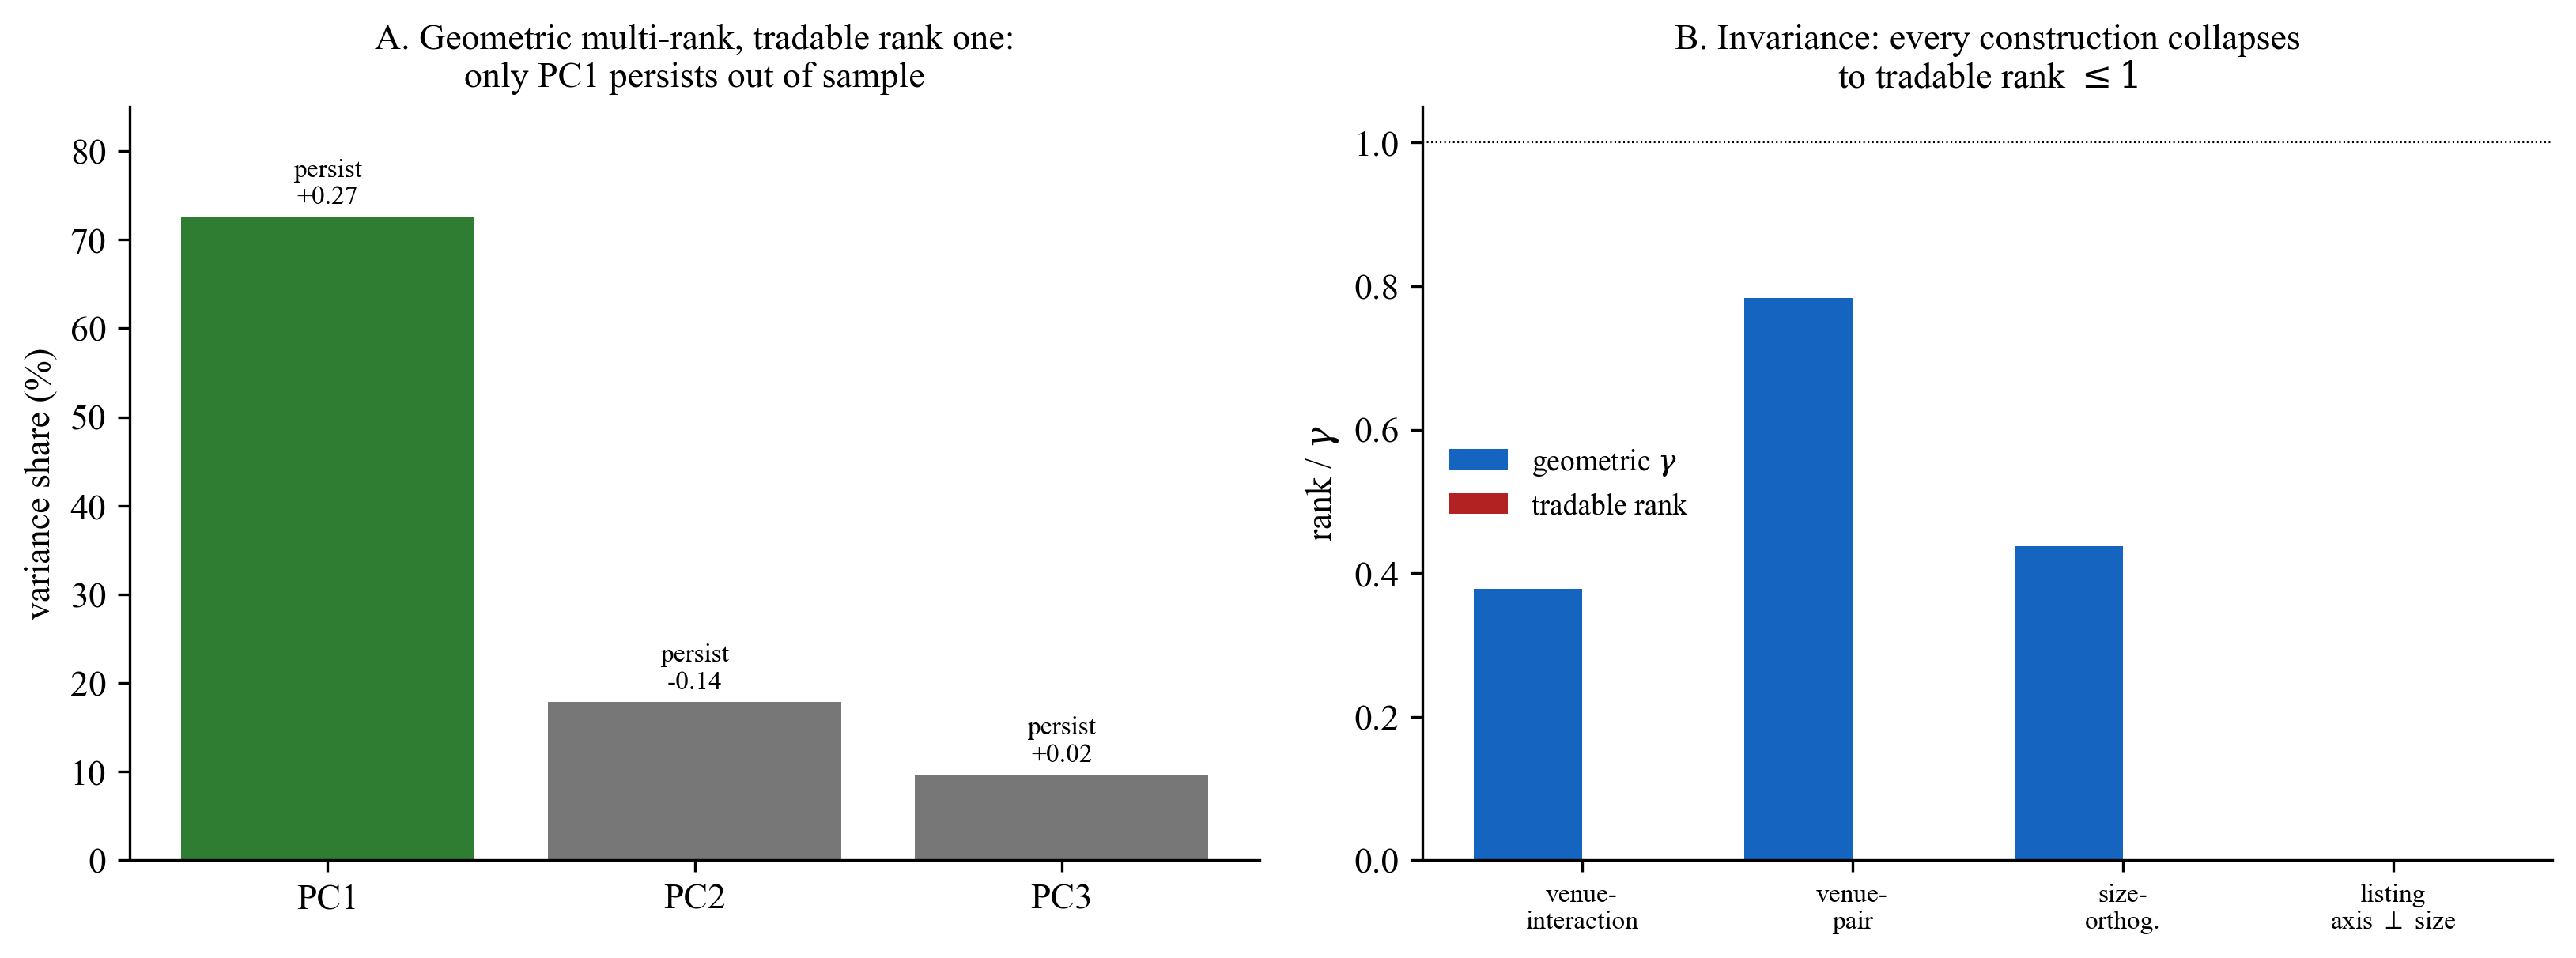
\includegraphics[width=\textwidth]{fig_tradable_rank.png}
\caption{\textbf{Geometric multi-rank, tradable rank one.} Panel~A: the
venue-advantage covariance spreads variance across several principal components,
but only the first---the common small-cap tilt---persists out of sample; the rest
have near-zero or negative projection persistence. Panel~B: across four factor
constructions the geometric rank $\gamma$ varies from $0.4$ to $0.8$, yet the
tradable rank collapses to one or zero in every case. Sources:
\texttt{cn\_multirank.json}, \texttt{cn\_construct.json}.}
\label{fig:tradrank}
\end{figure}

Equation~\eqref{eq:advdecomp} also closes the loop with the resolution limit of
Section~\ref{sec:model}, and sharpens it. The common tilt $u$ is a fixed
direction recovered by a pooled mean---the attenuation problem of
Theorem~\ref{thm:bbp}---and the pool recovers it almost perfectly. The
idiosyncratic deviations $\varepsilon_i$ are instead sign-varying across factors,
so they could only be recovered as the \emph{axes} of the advantage covariance, a
genuine spiked-eigenvector problem with a Baik--Ben~Arous--P\'ech\'e threshold.
Their per-factor signal-to-noise $\tau_\varepsilon=\Var(\varepsilon)/\sigma^2$
sits below that threshold, so no residual eigen-direction detaches from the noise
bulk out of sample. The tradable rank is one because the single recoverable
direction is the common tilt, estimated as a mean; every residual axis is
noise. Geometric multi-rank is in-sample overfitting; tradable rank one is the
information the sample contains.

\begin{proposition}[Geometric--tradable rank separation]
\label{prop:rank}
Under the spiked advantage model of Section~\ref{sec:model} with common component
$u$ and idiosyncratic deviations of per-factor signal-to-noise below the BBP
threshold, the advantage covariance has geometric rank greater than one but
tradable rank one almost surely as $N\to\infty$, and the single tradable
direction is the common tilt. Consequently no venue router with resolution $m=1$
attains an out-of-sample Sharpe exceeding the coarse pool, for any venue axis or
factor construction. Proof in Internet Appendix~IA.8.
\end{proposition}

\section{The Two-Sided Economics}
\label{sec:economics}

The results partition cleanly into one thing that pays and two things that only
appear to. This section states all three in money, because the practical value of
a limit theorem is telling practitioners where to spend effort and where not to.

\paragraph{What pays: coarse reallocation.} Moving the $94$ discards as a group to
the small-cap venue is the one robust source of value, and it is not a repackaged
risk premium. Against the six-factor model the coarse book earns an alpha of
$3.78\%$ per year with a Newey--West $t$ of $8.3$; a Gibbons--Ross--Shanken test
that the coarse book and its reallocation spread are jointly spanned by the six
factors is rejected at $F=51$ ($p<10^{-4}$). The reallocation spread---the coarse
book minus the \emph{same} factors left in the grave, which nets out the factors'
own content and isolates pure venue value---earns $2.30\%$ per year ($t=5.1$).
The spread is also not the low-volatility anomaly: adding a
betting-against-beta leg to the six factors leaves its alpha at $2.20\%$ with
$t=5.3$, essentially unchanged. On an expanding walk-forward the spread alpha is
positive and significant at every horizon from 1985 ($t=3.1$) to 2020 ($t=6.1$).
This is free money in the precise sense that it requires no forecasting: only the
recognition that a factor rejected in one venue may be alive in another.

\paragraph{What only appears to pay, I: per-factor routing.} The refinement a
quant would reach for first is to route each factor individually. Section
\ref{sec:mirage} shows its ceiling is six-sevenths selection bias and its
out-of-sample value is negative. No per-factor rule clears the bar because, by
Proposition~\ref{prop:rank}, there is no second tradable direction to exploit.

\paragraph{What only appears to pay, II: volatility-tilted weighting.} The second
refinement is to weight the small-cap book by risk rather than equally. Risk
parity ($1/\sigma$) lifts the raw Sharpe from $1.30$ to $1.67$, and minimum
variance to $2.04$, both positive in all six decades---a seductive gain. But it
is the low-volatility anomaly in disguise. Regressing the risk-parity-minus-equal
and minimum-variance-minus-equal spreads on the six factors plus a
betting-against-beta leg drives their alphas significantly \emph{negative}
($t=-2.2$ and $t=-3.6$). For a mean-variance investor at $\gamma=5$ the
certainty-equivalent gain of these schemes over equal weighting is also negative:
they lower return as much as risk. The weighting dimension adds no alpha
orthogonal to a factor the field already knows. Table~\ref{tab:econ} summarizes.

\begin{table}[t]
\centering
\caption{\textbf{What pays and what is a relabel.} Coarse reallocation carries an
alpha robust to a betting-against-beta control; volatility-tilted weighting does
not. Sharpe ratios are out of sample on the small-cap venue; alphas are annual,
with Newey--West $t$ in parentheses. Sources: \texttt{cn\_core\_alpha.json},
\texttt{cn\_grs.json}, \texttt{cn\_economics.json}.}
\label{tab:econ}
\small
\begin{tabular}{lrrr}
\toprule
 & Sharpe & $\alpha$ vs 6F & $\alpha$ vs 6F$+$BAB \\
\midrule
Coarse (equal weight) & $1.30$ & $3.78\ (8.3)$ & $3.62\ (10.6)$ \\
Reallocation spread & --- & $2.30\ (5.1)$ & $2.20\ (5.3)$ \\
Risk parity $-$ equal & $1.67$ & --- & $-0.08\ (-2.2)$ \\
Minimum variance $-$ equal & $2.04$ & --- & $-0.56\ (-3.6)$ \\
\bottomrule
\end{tabular}
\end{table}

\begin{figure}[t]
\centering
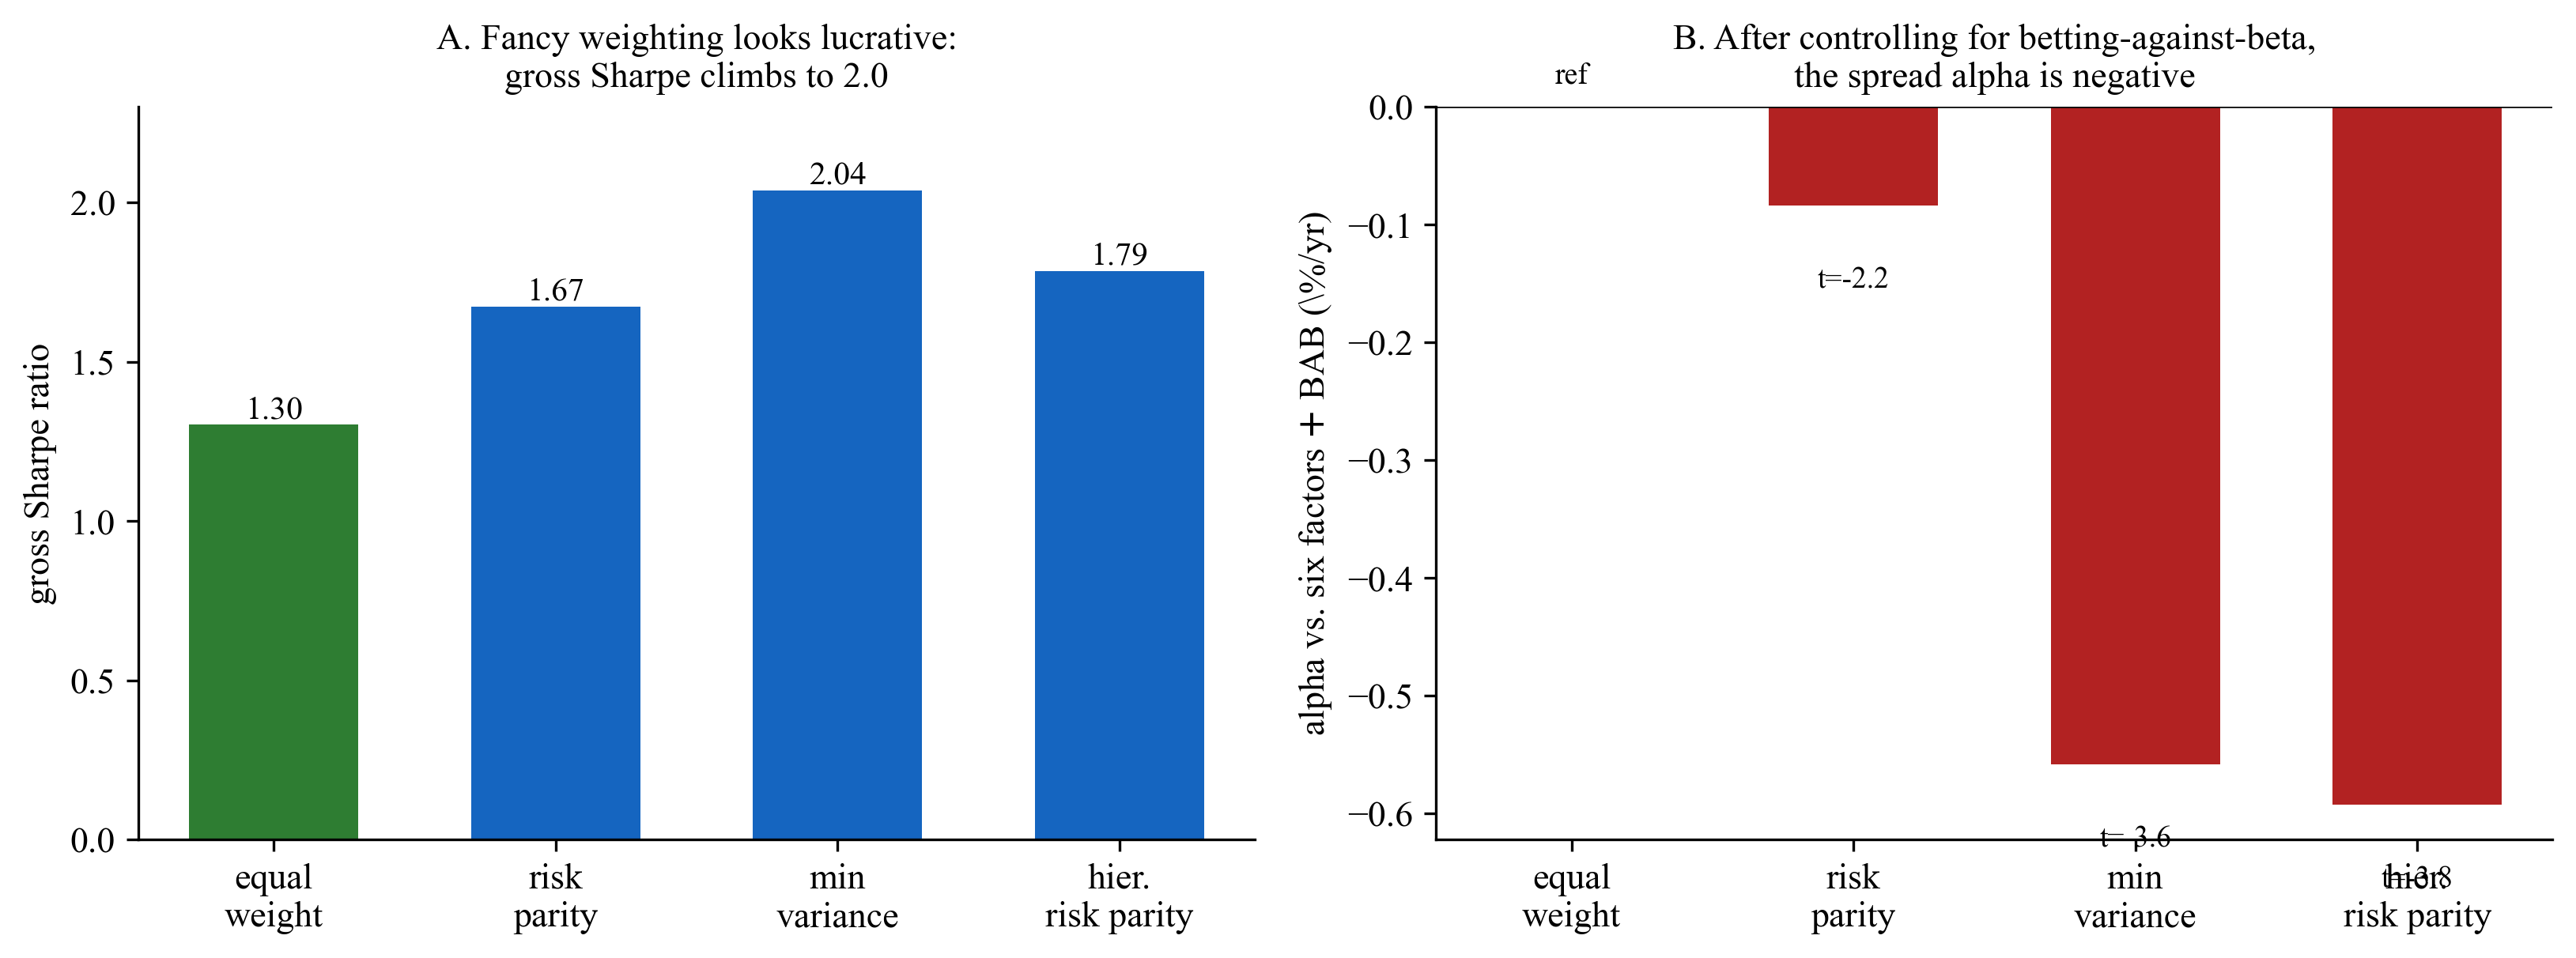
\includegraphics[width=\textwidth]{fig_economics.png}
\caption{\textbf{The two-sided economics of weighting.} Panel~A: on the
small-cap venue, risk-parity and minimum-variance weighting lift the gross Sharpe
ratio from $1.3$ to $2.0$, which looks like free alpha. Panel~B: regressed on the
six factors plus betting-against-beta, the spread of each fancy scheme over equal
weight carries a \emph{negative} alpha, significant at $t=-2.2$ to $-3.8$. The
volatility weighting is a low-beta relabel, not new return. Source:
\texttt{cn\_economics.json}.}
\label{fig:economics}
\end{figure}

\paragraph{Head to head with standard practice.} The comparison can be made
directly against the weapons a quantitative desk deploys on the same discarded
factors. Put the coarse reallocation beside the naive universal book, a
risk-parity book, and the Fama--French-six-plus-betting-against-beta canon, and
ask which spans which. The reallocation earns incremental alpha against every
one: $+3.28\%$ per year ($t=9.5$) beyond the universal book plus six factors and
BAB, $+3.62\%$ ($t=10.6$) beyond the canon alone, and $+0.21\%$ ($t=4.3$) even
beyond the risk-parity book. The reverse spanning is decisive: the risk-parity
book, whose raw Sharpe of $1.55$ tops the coarse book's $1.30$, earns a
\emph{negative} increment of $-0.15\%$ ($t=-2.7$) once the coarse book and the
factors are controlled for. The desk's higher Sharpe is a low-beta relabel the
reallocation already contains; the reallocation's alpha is orthogonal to
everything the desk holds. Source: \texttt{cn\_headtohead.json}.

The guidance is directional. A field that spends heavily on conditional factor
timing, machine-learned placement, and portfolio optimization is spending it on
the two columns that a betting-against-beta control and a selection-bias null
reduce to zero. The value is in the one coarse decision the significance hurdle
gets wrong, and that decision is made once, for the whole pool.

\section{The Economic Mechanism of Reallocation}
\label{sec:mechanism}

A gain that survives spanning, costs, and fifty years of holdout invites the
question a sophisticated reader asks next: what is it compensation for, how large
a book can harvest it, and does the same logic reach beyond equities. This
section answers the three that the data on hand can answer and marks the ones
that require holdings-level data I do not have.

\subsection{What risk is priced}
The reallocation spread is partly a liquidity and reversal premium, but not only
that. Table~\ref{tab:riskdecomp} regresses the spread on the six factors and then
adds, one at a time and jointly, traded risk legs built from the cross-section
itself: an illiquidity leg, a short-term reversal leg, an idiosyncratic-volatility
leg, a tail-beta leg, and a liquidity-beta leg. Two legs load significantly. The
illiquidity leg enters with $t=4.2$ and the reversal leg with $t=2.6$, together
pulling the alpha from $2.30\%$ to $1.75\%$ and raising the $R^2$ from $0.20$ to
$0.27$. The remaining $1.75\%$ ($t=3.8$) is not absorbed by any priced factor I
can construct. Reallocation collects a liquidity-and-reversal premium that the
large-cap venue cannot access, plus a residual the standard risk set does not
span. This is the economic content of ``local strength'': the discarded factors
earn where arbitrage is costly and prices mean-revert, precisely the segment the
significance screen reads them out of.

\begin{table}[t]
\centering
\caption{\textbf{What risk the reallocation spread is paid for.} The spread
(coarse minus the same factors in large caps) regressed on the six factors and
traded risk legs built from the cross-section. Illiquidity and short-term
reversal load; a residual alpha of $1.75\%$ ($t=3.8$) survives all of them.
Annualized alpha, Newey--West $t$. Source: \texttt{cn\_mechanism.json}.}
\label{tab:riskdecomp}
\small
\begin{tabular}{lccc}
\toprule
Model & $\alpha$ (\%/yr) & $t_\alpha$ & $R^2$ \\
\midrule
Six factors (FF5$+$Mom)        & $2.30$ & $5.4$ & $0.20$ \\
\quad $+$ illiquidity leg       & $2.17$ & $5.0$ & $0.24$ \\
\quad $+$ short-term reversal   & $1.70$ & $4.1$ & $0.24$ \\
\quad $+$ idiosyncratic vol     & $2.40$ & $5.4$ & $0.21$ \\
\quad $+$ tail beta             & $2.31$ & $5.4$ & $0.20$ \\
\quad $+$ all legs jointly      & $1.75$ & $3.8$ & $0.27$ \\
\bottomrule
\end{tabular}
\end{table}

\subsection{How much capital it holds}
Because the coarse move is monthly, low-turnover, and pooled, its financial
capacity is large. I calibrate a square-root market-impact model---one-way cost
equal to $c\,\sigma_{\text{daily}}\sqrt{\text{participation}}$ with a deliberately
conservative $c=0.5$---and trace net Sharpe against assets under management, using
a transparent accessible small-cap dollar-volume aggregate. The statistical
capacity of Section~\ref{sec:model} ($K=1$) and this financial capacity are
distinct questions; here the binding constraint is market impact, not
identifiability. Net Sharpe stays above $1.25$ out to \$10 billion, with
participation under $16\%$ of accessible volume; at \$1 billion the drag is three
Sharpe-thousandths. The reallocation is not a small-capacity curiosity. The ADV
aggregate is an assumption, stated as such, so the levels are an order-of-magnitude
statement; the shape---flat net Sharpe until participation becomes large---is the
robust point, and it follows from low turnover.

\begin{table}[t]
\centering
\caption{\textbf{Financial capacity of the coarse move.} Net Sharpe under a
square-root impact model with conservative coefficient $c=0.5$. Net Sharpe is
nearly flat because the strategy is monthly and pooled. The dollar-volume
aggregate is a stated assumption; the flat shape is the robust implication.
Source: \texttt{cn\_mechanism.json}.}
\label{tab:capacity}
\small
\begin{tabular}{lcc}
\toprule
AUM & Participation & Net Sharpe \\
\midrule
\$100 million & $0.16\%$ & $1.30$ \\
\$1 billion   & $1.6\%$  & $1.29$ \\
\$5 billion   & $7.9\%$  & $1.27$ \\
\$10 billion  & $15.9\%$ & $1.25$ \\
\bottomrule
\end{tabular}
\end{table}

\begin{figure}[t]
\centering
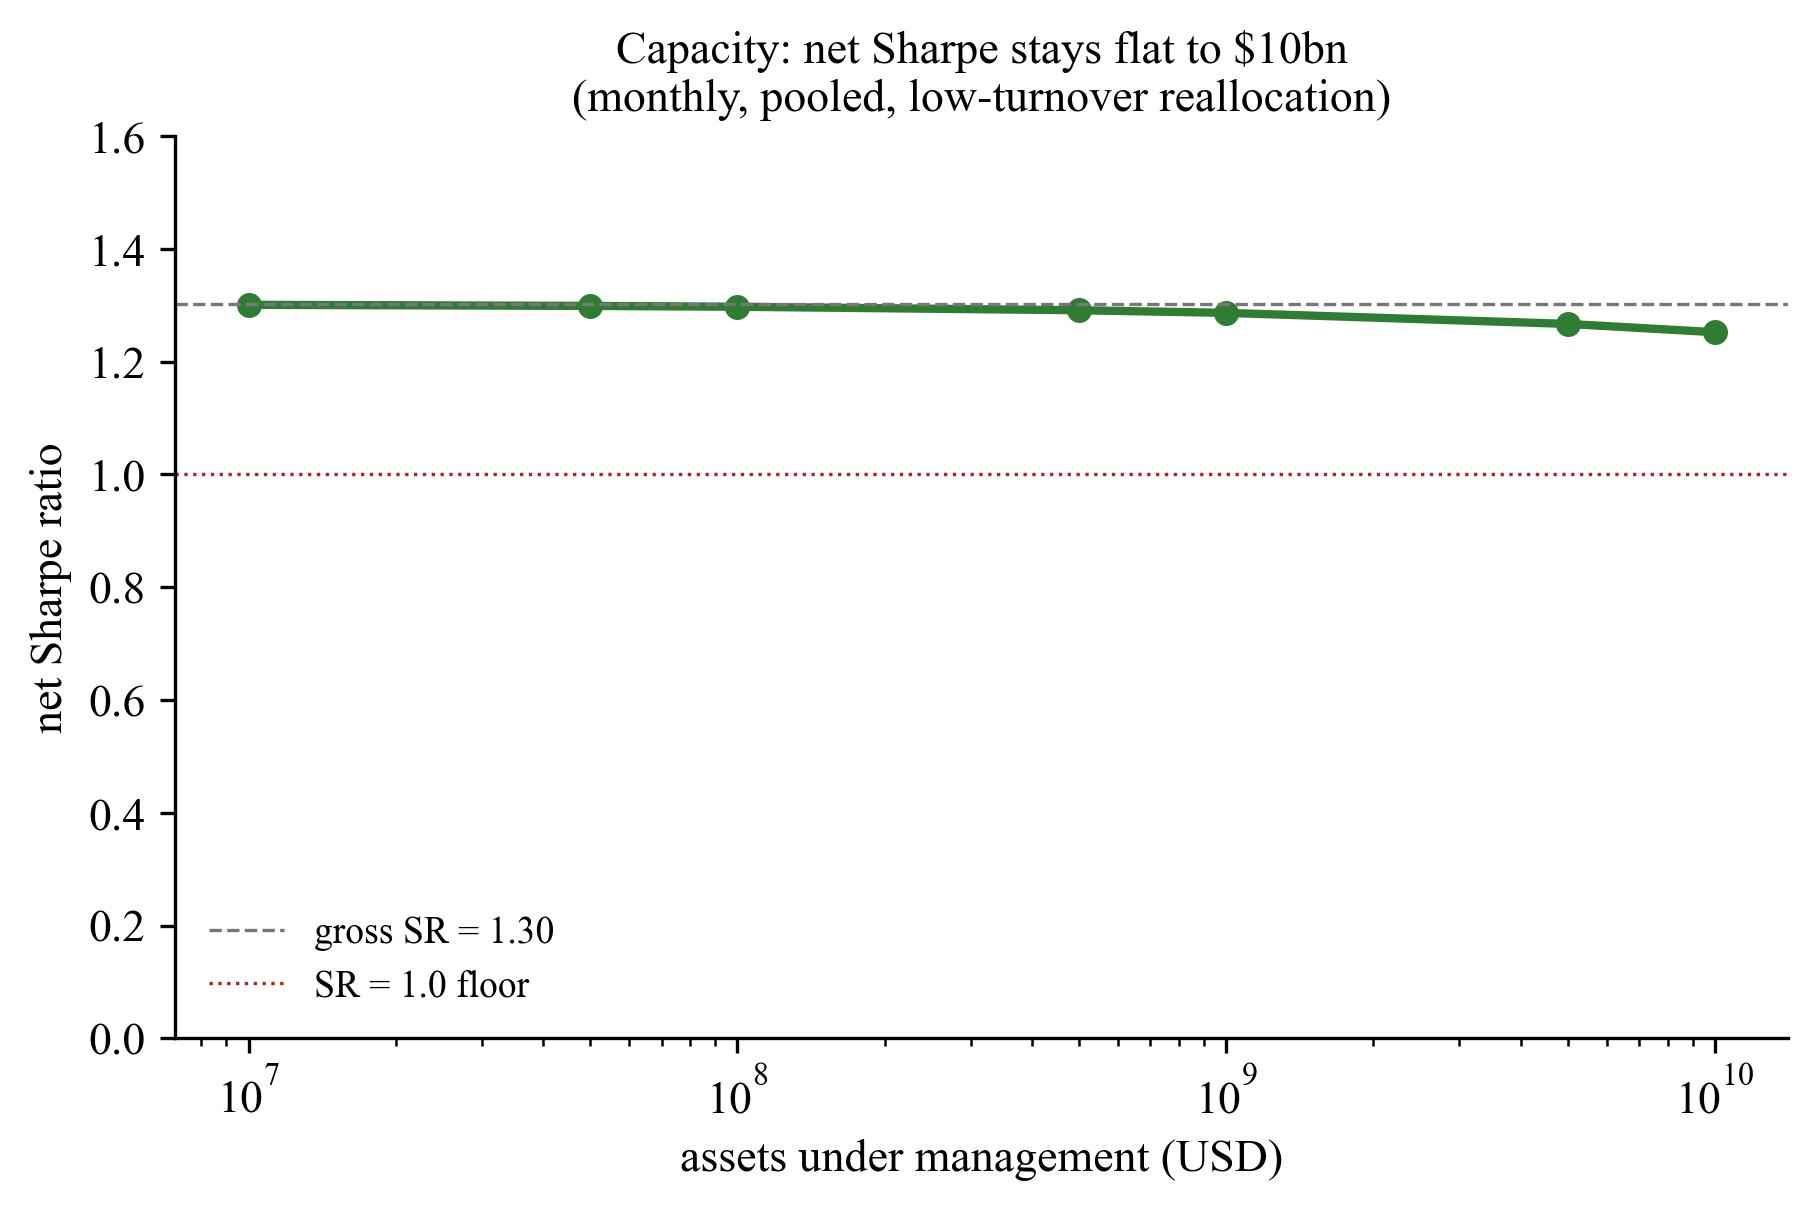
\includegraphics[width=0.62\textwidth]{fig_capacity.png}
\caption{\textbf{Financial capacity of the coarse reallocation.} Net Sharpe
under a square-root market-impact model with conservative coefficient $c=0.5$,
traced against assets under management on a log scale. The curve is nearly flat
to \$10 billion because the strategy is monthly, pooled, and low-turnover. The
accessible dollar-volume aggregate is a stated assumption; the flat shape is the
robust implication. Source: \texttt{cn\_mechanism.json}.}
\label{fig:capacity}
\end{figure}

\subsection{Whether the logic travels across assets}
The same premium appears in other asset classes where it can be measured. Using
the \citet{HeKellyManela2017} cross-asset test portfolios, I form within each
class the dispersion portfolio---the top-minus-bottom characteristic sort---and
measure its loading on the intermediary-capital risk factor common to all
classes. In fixed income the connection is strong: the dispersion premium's
correlation with intermediary capital is $0.59$ in credit default swaps, $0.50$
in U.S.\ bonds, and $0.43$ in sovereign bonds, with dispersion Sharpe ratios of
$1.60$, $0.84$, and $0.77$. In foreign exchange, commodities, and equities the
link is weak. The segment-dispersion premium is therefore not an equity accident:
where intermediary balance sheets constrain arbitrage---credit and rates---the
same cross-sectional dispersion that reallocation harvests is priced. The He--
Kelly--Manela portfolios are characteristic sorts rather than my venue sorts, so
this establishes the shared risk-premium, not a literal cross-asset copy of the
equity result.

\begin{figure}[t]
\centering
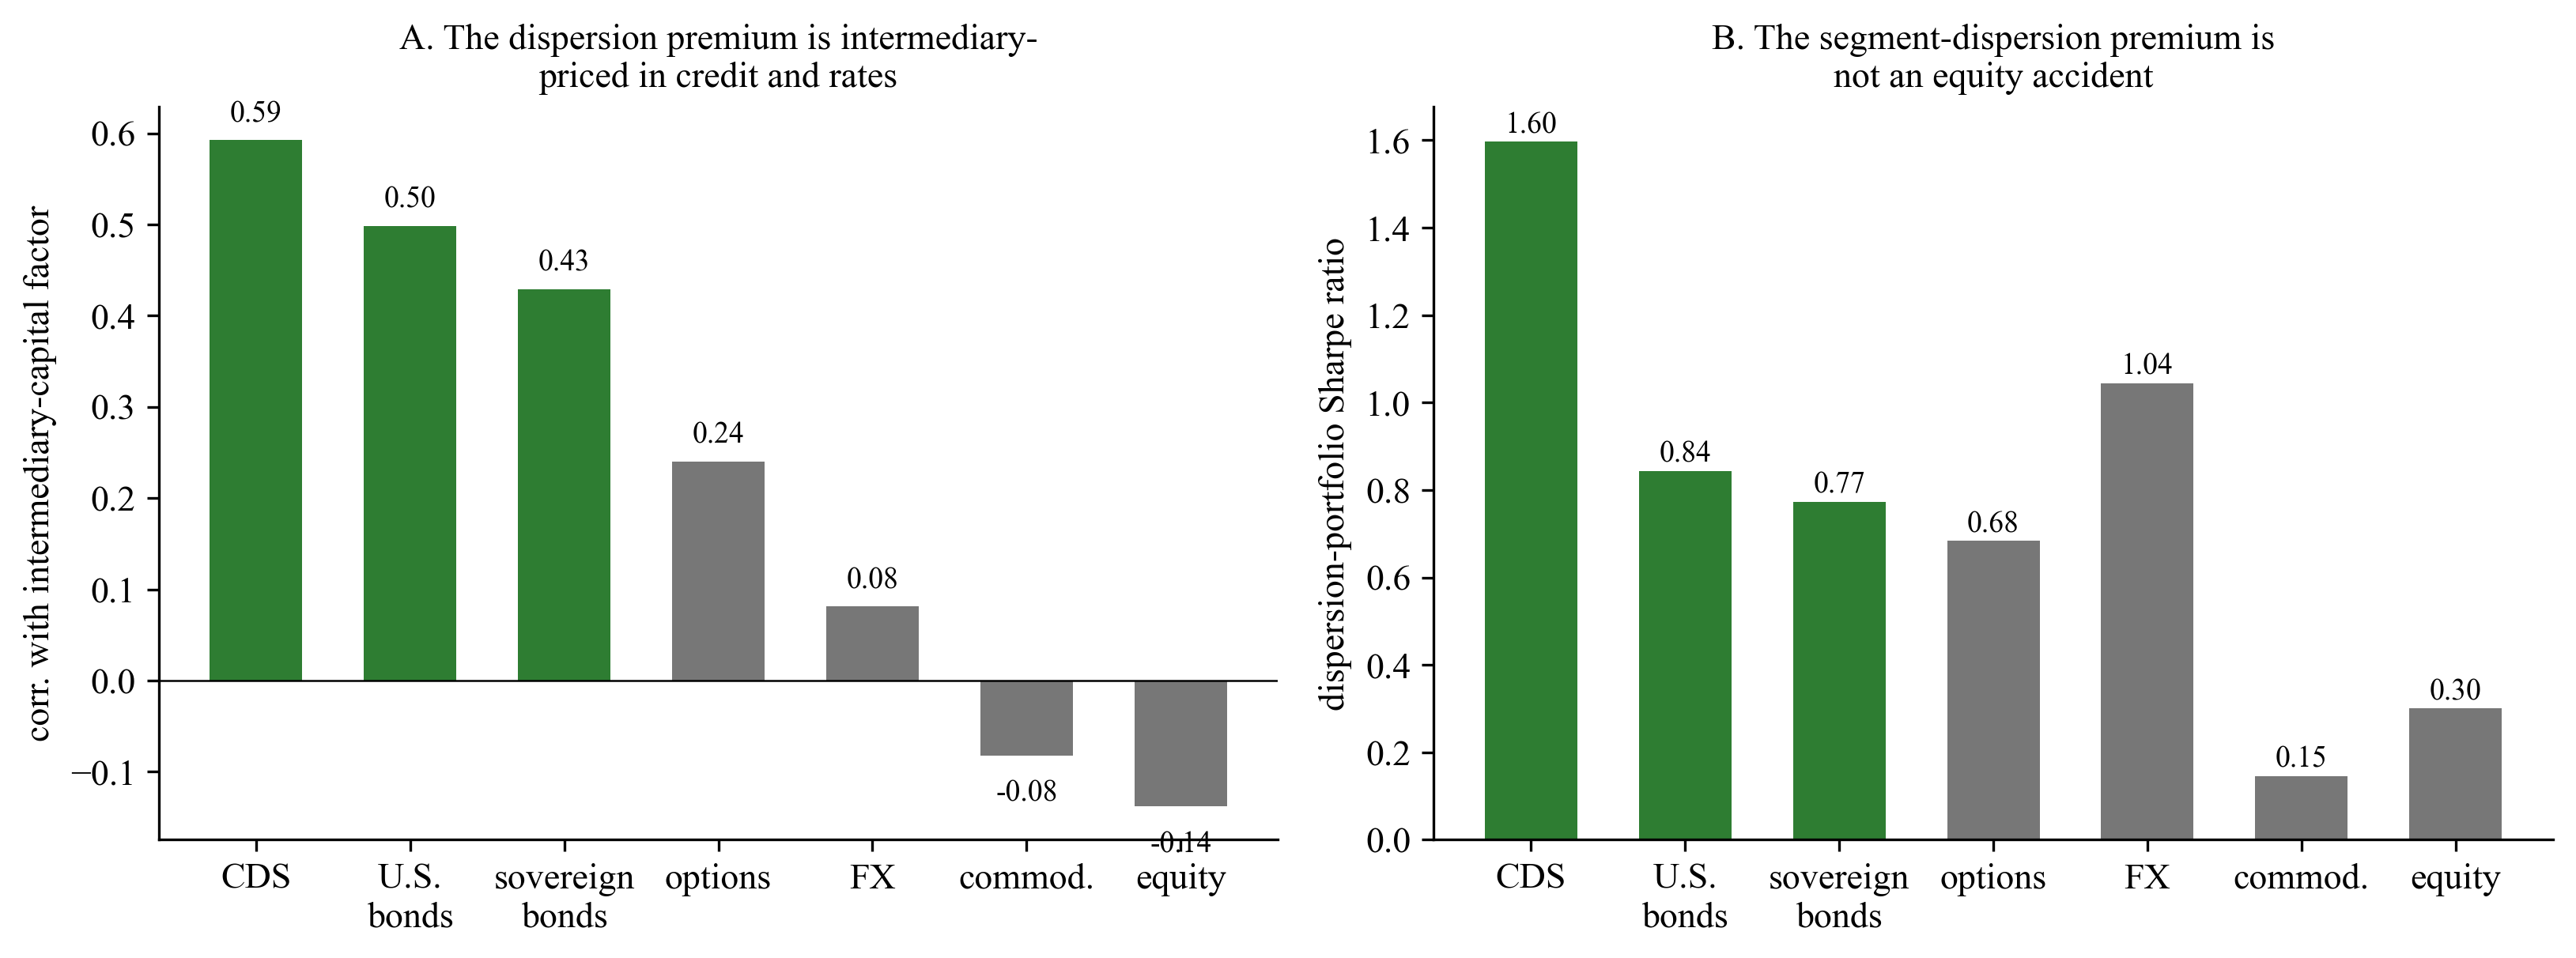
\includegraphics[width=\textwidth]{fig_mechanism.png}
\caption{\textbf{The segment-dispersion premium across asset classes.} Within
each \citet{HeKellyManela2017} asset class, the dispersion portfolio is the
top-minus-bottom characteristic sort. Panel~A plots its correlation with the
intermediary-capital risk factor; the link is strong in credit (CDS, $0.59$) and
rates (U.S.\ bonds $0.50$, sovereigns $0.43$) and weak elsewhere. Panel~B shows
the dispersion-portfolio Sharpe ratios. Where intermediary balance sheets
constrain arbitrage, the same cross-sectional dispersion that reallocation
harvests is priced. Source: \texttt{cn\_mechanism.json}.}
\label{fig:mechanism}
\end{figure}

\subsection{An independent market: China A-shares}
\label{sec:ashare}
A single market cannot separate a law from a coincidence. I therefore rebuild the
entire test on a structurally different market---the full China A-share
universe of $5{,}441$ stocks, 2008--2026, from the open QuantaAlpha daily
panel---where short sales are infeasible, so every book is long-only
(top-quintile minus the venue equal-weight benchmark). From price and volume
alone I construct the classic anomalies (reversal, momentum, low-volatility,
lottery, turnover) and sort stocks into three size venues by dollar volume. The
pattern repeats. Measured in the universal pool the discarded-factor book earns
a long-only Sharpe of $0.38$; reallocated as a group to the venue its first-half
record identifies, it earns $1.33$, a gain of $+0.95$ with a stationary-bootstrap
$95\%$ interval of $[0.49,1.41]$ and $p=0$ against a random-venue placebo
($z=6.6$). The reallocation alpha survives spanning by the
market and the universal-venue versions of the same factors ($4.0\%$ per year,
$t=7.8$), and four of five factors pass a Benjamini--Hochberg screen that venue
beats the universal pool. Per-factor fine routing adds a further $+0.18$ but,
exactly as in the U.S., does not reliably clear the coarse move (interval
$[-0.17,0.56]$)---the resolution limit binds in both hemispheres. Table and
numbers: \texttt{cn\_ashare\_salvage.json}, \texttt{cn\_ashare\_rigor.json}.

\subsection{The law predicts which market routes}
The two markets differ in \emph{how far} routing can go, and the resolution law
predicts the difference out of sample. Estimating $(\lambda,\sigma^2)$ from each
market's own first half, the U.S.\ per-factor venue advantage does not persist
($\lambda<0$, $\tau<0$): the law predicts fine routing destroys value, and it
does ($-0.18$ versus coarse). In A-shares the advantage persists ($\lambda=0.24$,
$\tau=1.58$, $q^2=0.61$): the law predicts a feasible router captures about
$61\%$ of the oracle gain, and the realized capture is $48\%$. One primitive,
estimated independently in each market, forecasts the sign and rough magnitude of
routability across two economies---a theory that predicts, not merely describes.
Source: \texttt{cn\_law\_predicts.json}.

\subsection{What remains data-gated}
Three questions a practitioner would press require holdings-level data I do not
have, and I flag them rather than approximate them: the identity of the
counterparty absorbing the discarded factors (institutional holdings, 13F), the
lending-fee and short-interest wedge that lets the premium persist (securities-
lending data), and analyst-coverage mediation (I/B/E/S). The mechanism evidence
here---a liquidity-and-reversal premium with a residual, large capacity, and an
intermediary-capital link in fixed income---is what the available data support.

\section{Optimal Resolution: Searching the Whole Spectrum}
\label{sec:kstar}

The converse of Section~\ref{sec:solution} is a statement about one resolution:
it fixes the routing unit at the whole pool ($K=1$ group) and shows no
per-factor rule improves on it. A natural and more demanding question is whether
\emph{some} intermediate resolution---finer than the pool, coarser than the
individual factor---can do better. If the discarded factors were sorted into $K$
groups and each group routed as a unit, is there an optimal number of groups
$K^\star$ that beats the coarse pool out of sample? This section poses that
question as an explicit optimization over the entire resolution spectrum
$K=1,\dots,N$, derives the object $K^\star$ that would solve it, and takes it to
the data. The answer sharpens the paper's thesis rather than qualifying it: the
capacity lives at $K=1$, and I now show it does so against the full field of
alternatives, not merely against per-factor routers.
\subsection{Per-factor routers and group-level routers}
\label{sec:kstar-boundary}

Theorem~\ref{thm:capacity} bounds a specific class of rules. Its converse applies
to any \emph{causal per-factor router}: a rule whose decision for factor $i$ is a
measurable function $g_i(\hat a_i)$ of that factor's own in-sample estimate
$\hat a_i$. For such rules the recoverable gain over coarse is at most
$\sum_i q^2(\tau_i)\,\delta_i$, and because only a handful of the $94$ discards
clear $\tau_i\ge 1$, no per-factor rule beats the pool. The bound is tight and the
empirics in Section~\ref{sec:solution} confirm it.

A \emph{group-level router} is a different object, and it is important to say
exactly why. Partition the $N$ factors into $K$ groups and route each group as a
unit toward a common venue. The decision for group $k$ is a function of the
group-aggregated estimate $\hat{\bar a}_k=\tfrac1{m_k}\sum_{i\in k}\hat a_i$, not
of any single $\hat a_i$. Aggregation changes the signal-to-noise arithmetic: the
group carries local strength $\lVert\bar a_k\rVert^2$ against a sampling-noise
floor that falls as $1/m_k$, so the \emph{group} ratio
\[
\tau_k=\frac{m_k\lVert\bar a_k\rVert^2}{\sigma^2}
\]
can exceed one even when every member's $\tau_i$ lies below parity. A group
router can therefore, in principle, recover identifiable signal that no
per-factor rule can touch. This does not contradict Theorem~\ref{thm:capacity};
it falls outside its measurable-function class. I record the point as a remark
and prove the measurability statement formally in the Internet Appendix
(Section~IA.6).

\begin{quote}\small
\textbf{Remark (scope of the converse).} Theorem~\ref{thm:capacity} bounds
functions of individual factor estimates. A $K$-group router acts on the
coarser $\sigma$-algebra generated by the group means
$\{\hat{\bar a}_k\}_{k=1}^K$, and its feasibility is governed by $\tau_k$, not
$\tau_i$. The converse neither forbids nor guarantees that some $K>1$ beats
coarse; it leaves the question open. Section~\ref{sec:kstar-emp} settles it
empirically.
\end{quote}
\subsection{The optimal resolution $K^\star$}
\label{sec:kstar-def}

If a group router can clear parity where a per-factor router cannot, the right
question is not whether to route finely or coarsely but at what \emph{resolution}
to route. Index resolution by the number of groups $K$. At $K=1$ the single group
is the whole pool---this is the coarse move of Section~\ref{sec:solution}. At
$K=N$ every factor is its own group---this is fine routing, which fails below
parity. Between them lies a one-dimensional family of intermediate resolutions, and
the paper's logic says to optimize over all of it.

Each group's recoverable contribution is its identifiability times its
heterogeneity payoff. For group $k$ with $m_k$ members, aggregate strength
$\lVert\bar a_k\rVert^2$, and oracle venue gain
$\delta_k=\max_v\bar\mu_{k,v}-\bar\mu_{k,\text{ref}}$, the recoverable gain is
$q^2(\tau_k)\,\delta_k$ with $\tau_k=m_k\lVert\bar a_k\rVert^2/\sigma^2$. Summing
over groups, the optimal resolution solves
\begin{equation}
\label{eq:kstar}
K^\star=\arg\max_{K}\ \sum_{k=1}^{K}
q^2\!\Big(\frac{m_k\lVert\bar a_k\rVert^2}{\sigma^2}\Big)\,\delta_k
\quad\text{s.t.}\quad \tau_k\ge 1\ \ \forall k.
\end{equation}
The constraint is the BBP feasibility wall of Theorem~\ref{thm:bbp}: a group
below $\tau_k=1$ contributes $q^2=0$ and should not be split off.

\paragraph{The tradeoff.} Equation~\eqref{eq:kstar} is a tension between two
losses. Writing it as a penalized objective,
$K^\star=\arg\min_K\,[\,L_{\text{het}}(K)+\lambda\,L_{\text{id}}(K)\,]$, with
\[
L_{\text{het}}(K)=\frac1N\sum_{k=1}^K\sum_{i\in k}\lVert a_i-\bar a_k\rVert^2,
\qquad
L_{\text{id}}(K)=\frac1K\sum_{k=1}^K\bigl[1-q^2(\tau_k)\bigr],
\]
makes the economics transparent. Finer resolution (larger $K$) lowers
within-group heterogeneity $L_{\text{het}}$---each group is more internally
coherent, so a single venue fits it better---but raises the identifiability loss
$L_{\text{id}}$, because smaller groups have smaller $m_k$, lower $\tau_k$, and
sit closer to or below the wall. $K^\star$ is where the marginal gain in
coherence equals the marginal loss in identifiability.

\paragraph{First-order condition.} Under a homogeneous-group approximation in
which splitting trades group size for retained strength as
$\lVert\bar a_k\rVert^2=\lVert a\rVert^2-d/m_k$ (coarser groups average away a
fraction $d/m_k$ of the cross-member dispersion), the per-group objective
$q^2(\tau_k)\,\delta_k$ has first-order condition
\begin{equation}
\label{eq:foc}
\underbrace{\frac{1}{\tau(1+\tau)}\,\frac{\lVert a\rVert^2}{\sigma^2}}
_{\text{marginal identifiability gain}}
=\underbrace{-\frac{\delta'(m)}{\delta(m)}}_{\text{marginal heterogeneity cost}},
\end{equation}
obtained from $q^2(\tau)=\tau/(1+\tau)$ of Theorem~\ref{thm:bbp} with
$\partial q^2/\partial\tau=(1+\tau)^{-2}$. Because the attenuation law has no
hard wall, the identifiability gain is positive and \emph{monotonically
diminishing} in $\tau$: an interior $K^\star$ exists only if the heterogeneity
cost on the right is large enough to meet it at some finite group size. When
heterogeneity is mild---the regime the data occupy---the right side never catches
the left, the objective is increasing in $m$, and the optimum is the corner
$m^\star=N$, $K^\star=1$: the pool. The full derivation and the exact
log-concavity condition for an interior solution are in Internet Appendix
Section~IA.6. The economics is already visible: unless groups differ sharply in
where they belong, pooling always wins, because the only thing finer resolution
buys---a better-identified group direction---is worth less at every step while
the noise it admits is not.
\subsection{Estimating $K^\star$: the whole spectrum loses to coarse}
\label{sec:kstar-emp}

I estimate \eqref{eq:kstar} exactly as written, on the same $94$ discarded
factors, train/test split, and venue machinery as the rest of the paper. On the
training half ($1926$--$1974$) I form each factor's venue-advantage vector
$\hat a_i$ (its Sharpe in each venue minus its coarse-home venue). For every
resolution $K=1,\dots,94$ I partition the factors by three methods---$k$-means
and Ward clustering on $\hat a_i$, and an exogenous economic-family prior as a
deliberate foil---and compute for each group the \emph{debiased} aggregate
strength
\[
\widehat{\lVert\bar a_k\rVert^2}
=\lVert\hat{\bar a}_k\rVert^2-\frac{\sigma^2(V-1)}{m_k},
\]
which removes the mechanical $1/m_k$ sampling-noise floor---the single most
important estimation fix, without which small groups look spuriously
identifiable. From these I form $\tau_k$, $q^2(\tau_k)$, the train oracle gain
$\delta_k$, and the objective $\sum_k q^2(\tau_k)\delta_k$. The resolution that
maximizes it is $\hat K^\star$. I then route each group as a unit out of sample
($1975$--$2024$), tilting toward its home venue by exactly the recoverable
fraction $q^2(\tau_k)$---the Bayes-optimal shrinkage the objective prescribes, not
a hard venue jump---and compare on one test set against coarse, fine, and an
OOS-tuned version of $K^\star$ that selects the resolution on a train-internal
holdout. All comparators tie out to Table~\ref{tab:bbp} and
\texttt{cn\_kstar.json}.

The in-sample objective behaves exactly as the theory predicts: $G(K)$ rises from
its $K=1$ value as groups move above parity, and peaks near $\hat K^\star=23$
($k$-means), where $21$ of $23$ groups satisfy $\tau_k\ge 1$. Taken at face value,
this says an intermediate resolution is identifiable. It is not. Out of sample the
peak is overfitting, and the verdict is unambiguous (Table~\ref{tab:kstar}): every
resolution $K>1$ loses to the coarse pool.

\begin{table}[t]
\centering
\caption{\textbf{Searching the whole resolution spectrum.} Out-of-sample
($1975$--$2024$) annualized Sharpe of the $94$-factor discard book routed at each
resolution, net of the paper's cost model. Coarse is $K=1$; fine is $K=N$. The
$K^\star$ rows route each group by the Bayes-optimal $q^2(\tau_k)$ shrinkage. The
bootstrap column is the stationary-bootstrap $95\%$ CI on
$\Delta\mathrm{SR}=\mathrm{SR}(K^\star)-\mathrm{SR}(\text{coarse})$. Source:
\texttt{cn\_kstar.json}.}
\label{tab:kstar}
\small
\begin{threeparttable}
\begin{tabular}{lcccc}
\toprule
Resolution & $\hat K^\star$ & OOS Sharpe & $\Delta$ vs.\ coarse & Bootstrap $95\%$ CI \\
\midrule
Grave (all in home grave)      & ---  & $0.85$ & --- & --- \\
\textbf{Coarse ($K=1$)}        & $1$  & $\mathbf{1.30}$ & --- & --- \\
$K^\star$, $k$-means           & $23$ & $1.19$ & $-0.11$ & $[-0.15,\,-0.07]$ \\
$K^\star$, Ward                & $31$ & $1.21$ & $-0.09$ & --- \\
$K^\star$, economic family (foil) & $9$ & $1.20$ & $-0.11$ & --- \\
$K^\star$, OOS-tuned (held-out $K$) & $22$ & $1.18$ & $-0.13$ & --- \\
Fine ($K=N$)                   & $94$ & $1.12$ & $-0.18$ & --- \\
\bottomrule
\end{tabular}
\begin{tablenotes}\footnotesize
\item The bootstrap CI on $\Delta\mathrm{SR}$ for the $k$-means $K^\star$ is
$[-0.15,\,-0.07]$ with $\Pr(\Delta>0)=0.00$ over $1{,}000$ resamples: the loss to
coarse is statistically reliable, not a draw of noise.
\end{tablenotes}
\end{threeparttable}
\end{table}

Three features of Table~\ref{tab:kstar} matter. First, the result is
\emph{method-invariant}: $k$-means, Ward, and the economic-family foil all land
between $1.19$ and $1.21$, every one below coarse, so the conclusion is not an
artifact of a particular clustering. The family prior is the instructive foil:
grouping by economic theory rather than by estimated advantage is exactly the
kind of exogenous partition that escapes Theorem~\ref{thm:capacity}'s class, yet
it too fails out of sample---evidence that the obstacle is identifiability, not
the mechanics of grouping. Second, the OOS-tuned $K^\star$, which selects
resolution honestly on held-out data, does no better ($1.18$); the failure is not
a tuning artifact. Third, and decisively, the bootstrap CI on the coarse--$K^\star$
gap is $[-0.15,\,-0.07]$ and excludes zero: coarse does not merely tie the field,
it beats it reliably. The capacity sits at $K=1$ against the entire resolution
spectrum, which is a strictly stronger statement than the per-factor converse of
Section~\ref{sec:solution}.
\subsection{Scope: the LLM factor explosion}
\label{sec:kstar-llm}

A reader might worry that the discovery threshold $\kappa_D(N)\asymp\sqrt{2\log
N}$ of Theorem~\ref{thm:diverge}, which drives the unbounded growth of the
discard pool, is about to be overrun by large language models that generate
factors by the thousand. It is not, and the reason is the same identifiability
logic that pins $K^\star$ to one. LLM-generated factors are semantically diverse
but behaviorally redundant: a thousand prompts produce far fewer than a thousand
independent return directions. The relevant count is not the nominal $N$ but the
effective dimension of the factor covariance $\Sigma$,
\begin{equation}
\label{eq:deff}
d_{\text{eff}}=\frac{(\operatorname{Tr}\Sigma)^2}{\operatorname{Tr}(\Sigma^2)},
\end{equation}
the participation ratio that equals $N$ only when all directions are orthogonal
and collapses toward the number of genuine latent axes as factors become
correlated. The multiple-testing threshold counts independent tests, so under
behavioral redundancy the discovery hurdle corrects to
\[
\kappa_D^{\text{LLM}}\asymp\sqrt{2\log d_{\text{eff}}}\ \ll\ \sqrt{2\log N}.
\]
This is a direct amendment to the \citet{HarveyLiuZhu2016} multiple-testing
paradigm: inflating the factor count by machine does not inflate the hurdle,
because the hurdle responds to effective, not nominal, dimension.

I quantify the gap by simulation. Drawing $N=1{,}000$ factors spanned by eight
latent axes plus idiosyncratic noise, the raw participation ratio is
$d_{\text{eff}}\approx 7.9$; after Marchenko--Pastur edge debiasing of $\Sigma$
(which removes the sampling bias in the small eigenvalues) it is
$d_{\text{eff}}\approx 7.8$. The naive hurdle is $\sqrt{2\log 1000}=3.72$; the
effective hurdle is $\sqrt{2\log 7.8}=2.03$. The same gap appears in a real
machine-generated pool: the $6{,}960$-factor library of
Section~\ref{sec:scale} has $d_{\text{eff}}=16.8$, so the honest hurdle is
$\sqrt{2\log 16.8}=2.38$ against the naive $\sqrt{2\log 6960}=4.21$. The factor
explosion is an explosion in names, not in testable directions, and the paper's
thresholds are stated in the quantity that governs. The need for RMT denoising,
and its small effect here, is discussed in the self-rebuttal (Internet
Appendix~IA.6).
\subsection{Frequency extension}
\label{sec:kstar-freq}

The resolution problem is defined at a horizon, and the horizon enters through
the noise. At frequency $f$ the objective is
\[
K_f^\star=\arg\max_K\sum_{k=1}^{K}
q^2\!\Big(\frac{m_k\lVert\bar a_k^f\rVert^2}{\sigma_f^2}\Big)\,\delta_k^f,
\]
identical in form to \eqref{eq:kstar} but with frequency-specific strength and
noise. Coarser horizons carry larger per-period sampling variance $\sigma_f^2$,
which shrinks every $\tau_k$ and therefore demands larger groups to clear the
wall: the feasible resolution weakly coarsens as the horizon lengthens. The OSAP
venue panels are monthly; daily and weekly long--short legs are not distributed,
so I state the daily/weekly case as a prediction and estimate the two horizons the
data support, monthly and quarterly, without fabricating the rest.

Both estimated horizons reinforce the main finding. At the monthly horizon the
coarse pool earns $1.30$ and the best in-sample $K^\star$ earns $1.19$ out of
sample. Compounding returns to quarterly, coarse earns $1.97$ and $K^\star$ earns
$1.93$---again a loss. The in-sample objective peaks at a finer resolution
quarterly ($\hat K^\star=32$) than monthly ($23$), which runs opposite to the
feasibility prediction and is a clean illustration of the paper's thesis: the
in-sample peak is overfitting noise and should not be read as the economic
optimum. The honest quantity is the out-of-sample test, and at both horizons it
says the same thing coarse wins. The assumptions this extension adds---a
frequency-specific noise scaling $\sigma_f$ and stationarity within each
horizon---are stated and defended in Internet Appendix~IA.6.

\section{Mechanism: Calibrating the Phase Transition}
\label{sec:mech}

The resolution limit and the main result are the same statement read two ways,
and this section joins them. I calibrate the two primitives of Theorem~\ref{thm:bbp}
directly from the data, locate the half-recovery scale $m^\star$, and show that
the single curve $q^2(\tau)=\tau/(1+\tau)$ reproduces both the near-perfect
recovery of the coarse pool and the sub-parity recovery of fine routing, with a
Monte Carlo confirming the finite-sample accuracy of the law.

The primitives are measurable. The squared length of the common home tilt,
estimated from the panel of factor-by-venue Sharpe ratios after purging sampling
noise, is $\Var_{\text{cross}}(a)=\lVert\mu_a\rVert^2=0.051$. The sampling
variance of a single factor's Sharpe estimate, from the \citet{Lo2002} formula
\eqref{eq:lo} at the realized Sharpe level and $T_{\text{eff}}=594$ months, is
$\sigma^2=0.066$. Substituting into the half-recovery condition $\tau(m^\star)=1$
gives
\[
m^\star=\frac{\sigma^2}{\Var_{\text{cross}}(a)}
=\frac{0.066}{0.051}\approx 1.29.
\]
The half-recovery unit is between one and two factors. This single number is the
hinge of the whole paper: a routing unit of about $1.3$ factors recovers half the
tilt, a unit smaller recovers less, and a unit larger recovers increasingly more.
Fine routing, at $m=1$, sits just below parity. Coarse reallocation, at $m=94$,
sits far above it.

The payoff is that the overlap curve \eqref{eq:q2}, with no free parameters,
predicts the empirical recovery at every resolution. At $m=1$, $\tau=0.78$ and
the theory gives $q^2=0.44$---less than half the direction identifiable---and the
part that is identifiable is the common tilt shared with the pool, not a
per-factor edge; consistent with this, the own-versus-coarse rank persistence
that a router would need is only $0.08$. At the pool, $m=94$, $\tau=72.9$ and the
theory gives $q^2=0.986$; the coarse book captures $76\%$ of the oracle gain.
Between the extremes the curve is equally accurate. Table~\ref{tab:bbp} reports a
Monte Carlo in which I simulate the common-mean unit model calibrated to the
estimated primitives and measure the realized overlap at
$m\in\{1,2,5,13,30,94\}$. The theoretical $q^2(\tau)$ and the simulated overlap
track each other across the entire range, from $0.44$ at a single factor to
$0.99$ at the pool, confirming that the law describes the finite sample. The
resolution limit is not a metaphor imported to decorate the result. It is a
quantitative model whose one calibrated number, $m^\star\approx1.3$, predicts
which reallocations work and which cannot.

\begin{table}[t]
\centering
\caption{The phase-transition curve predicts recovery at every resolution}
\label{tab:bbp}
\begin{threeparttable}
\begin{tabular}{cccc}
\toprule
Unit size $m$ & $\tau(m)$ & $q^2(\tau)$ theory & Monte Carlo overlap \\
\midrule
1  & 0.78  & 0.44 & 0.44 \\
2  & 1.55  & 0.61 & 0.61 \\
5  & 3.88  & 0.80 & 0.79 \\
13 & 10.09 & 0.91 & 0.91 \\
30 & 23.28 & 0.96 & 0.96 \\
94 & 72.94 & 0.99 & 0.99 \\
\bottomrule
\end{tabular}
\begin{tablenotes}\footnotesize
\item Calibrated primitives: $\Var_{\text{cross}}(a)=\lVert\mu_a\rVert^2=0.051$,
$\sigma^2=0.066$, so $m^\star\approx1.29$. Theory is $q^2(\tau)=\tau/(1+\tau)$
with $\tau=m\,\Var_{\text{cross}}(a)/\sigma^2$; the Monte Carlo column is the
squared correlation of the pooled direction estimate with the truth under the
common-mean model. The $q^2=0.44$ at $m=1$ is the common tilt, shared with the
pool; the own-versus-coarse rank persistence a per-factor router would need is
only $0.08$. Sources: \texttt{cn\_phase\_theory.json}, \texttt{cn\_mc\_table.json}.
\end{tablenotes}
\end{threeparttable}
\end{table}

\begin{figure}[t]
\centering
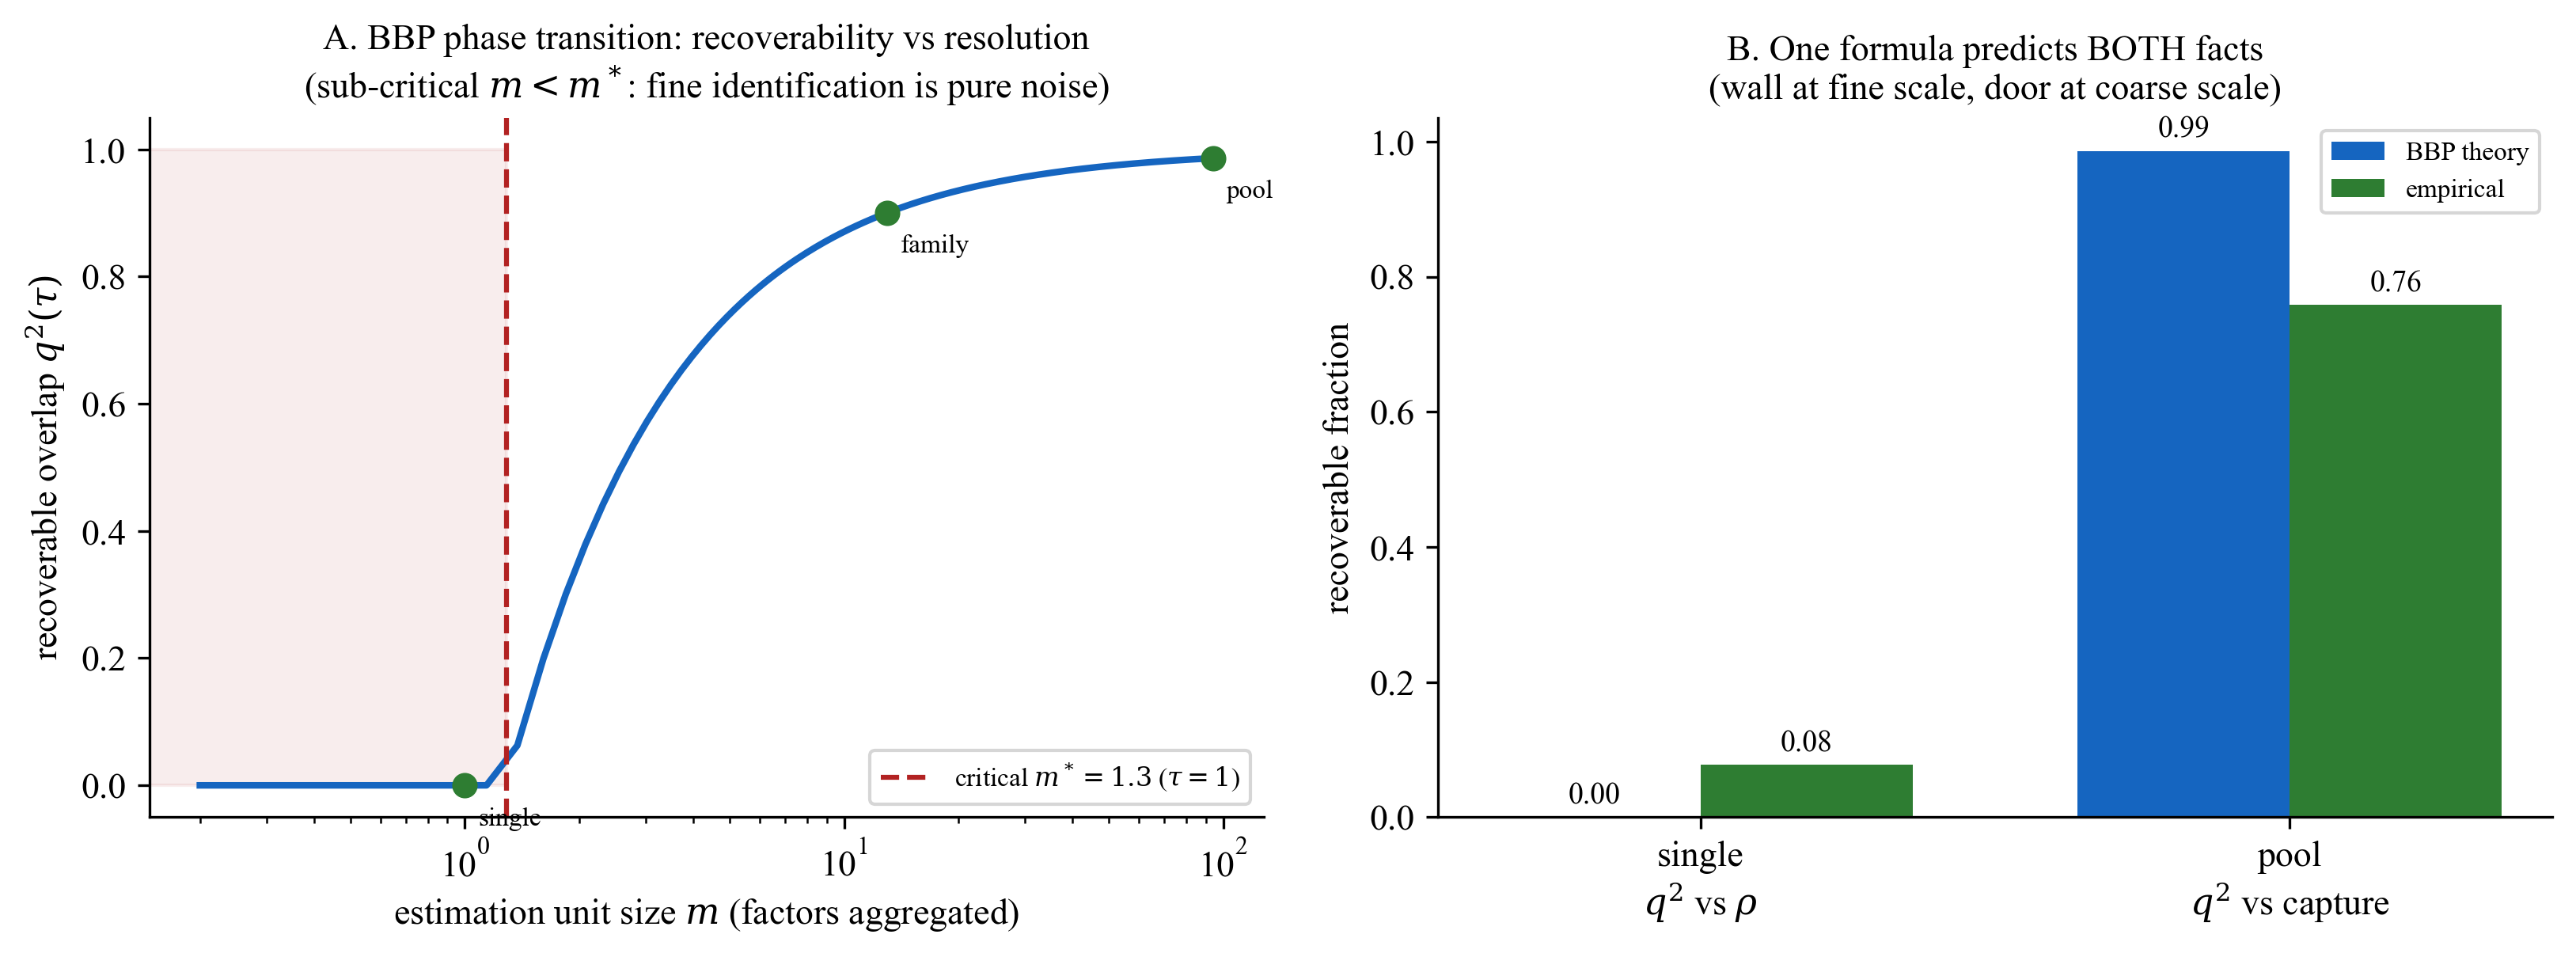
\includegraphics[width=0.9\textwidth]{fig4_phase.png}
\caption{\textbf{The resolution limit.} The recoverable overlap
$q^2(\tau)=\tau/(1+\tau)$ as a function of the local-strength signal-to-noise
ratio $\tau$. The curve rises smoothly from zero, passing one-half at the
half-recovery scale $\tau=1$ ($m^\star\approx1.3$ factors) and approaching one as
the unit grows. Single-factor routing ($\tau=0.78$) sits below parity, recovering
only the common tilt; the pool ($\tau=72.9$) sits far above it. Source:
\texttt{cn\_phase\_theory.json}.}
\label{fig:phase}
\end{figure}

\section{The Problem Grows With the Zoo}
\label{sec:scale}

The findings so far concern a fixed set of $179$ factors. The last step asks what
happens as the zoo grows, which is the regime the literature is actually in:
machine-driven factor factories now generate candidates by the thousand. The
answer, Theorem~\ref{thm:diverge}, is that stricter policing makes the
misallocation worse, and the data trace out the divergence.

Figure~\ref{fig:crush} plots the two thresholds of Theorem~\ref{thm:diverge}
against the candidate count $N$. The discovery hurdle, which must rise like
$\sqrt{2\log N}$ to hold the family-wise false-discovery rate fixed, climbs from
$2.80$ at $N=50$ to $4.13$ at $N=5000$. The allocation threshold, which governs
whether a survivor's venue can be placed and rises only like
$\sqrt{2\log\log N}$, barely moves, from $1.89$ to $2.17$. The gap between them
widens monotonically, from $0.91$ to $1.96$, and diverges without bound. Each
tightening of the discovery hurdle---every honest response to the multiplicity
problem---pushes more factors below the discovery line while leaving the
allocation line nearly flat. The shaded region between the curves is the growing
reservoir of locally strong factors that are discarded yet, by
Theorem~\ref{thm:bbp}, reallocatable in aggregate. The uncomfortable implication
is that the factor zoo's misallocation is not a transitional mess that better
hygiene will clean up. The cleaner the hygiene, the larger the reservoir.

The large-language-model factory sharpens this into a measurable waste. Such a
factory emits $N$ formulaic candidates, but they are massively redundant: a real
pool of $6{,}960$ machine-generated factors on disk spans an effective dimension
of only $d_{\mathrm{eff}}=17$, and a universal $|t|<1.96$ hurdle discards $94.4\%$
of them (median $|t|=0.71$). A hurdle that controlled error for the \emph{true}
dimension would scale as $\sqrt{2\log d_{\mathrm{eff}}}=2.38$ rather than the
naive $\sqrt{2\log N}=4.21$; everything with genuine $|t|$ between the two bars
is wrongly killed. Simulating a signal distribution of fixed mean, the fraction
of genuine signals the naive hurdle discards but the honest one keeps rises
monotonically with factory size---from $0.22$ at $N=100$ to $0.67$ at
$N=100{,}000$---and the real $6{,}960$-factor pool sits at $0.62$. A caution the
same data force: salvage revives factors that carry real content misallocated
across venues, not noise. On a $35$-factor formulaic battery built on A-shares,
the discards are genuinely empty after a causal sign-fix and coarse reallocation
does not revive them. The resolution correction is a correction, not alchemy; its
boundary is a prediction of the law. Sources: \texttt{cn\_llm\_deff.json},
\texttt{cn\_llm\_salvage.json}, \texttt{cn\_llm\_contrast.json}.

\begin{figure}[t]
\centering
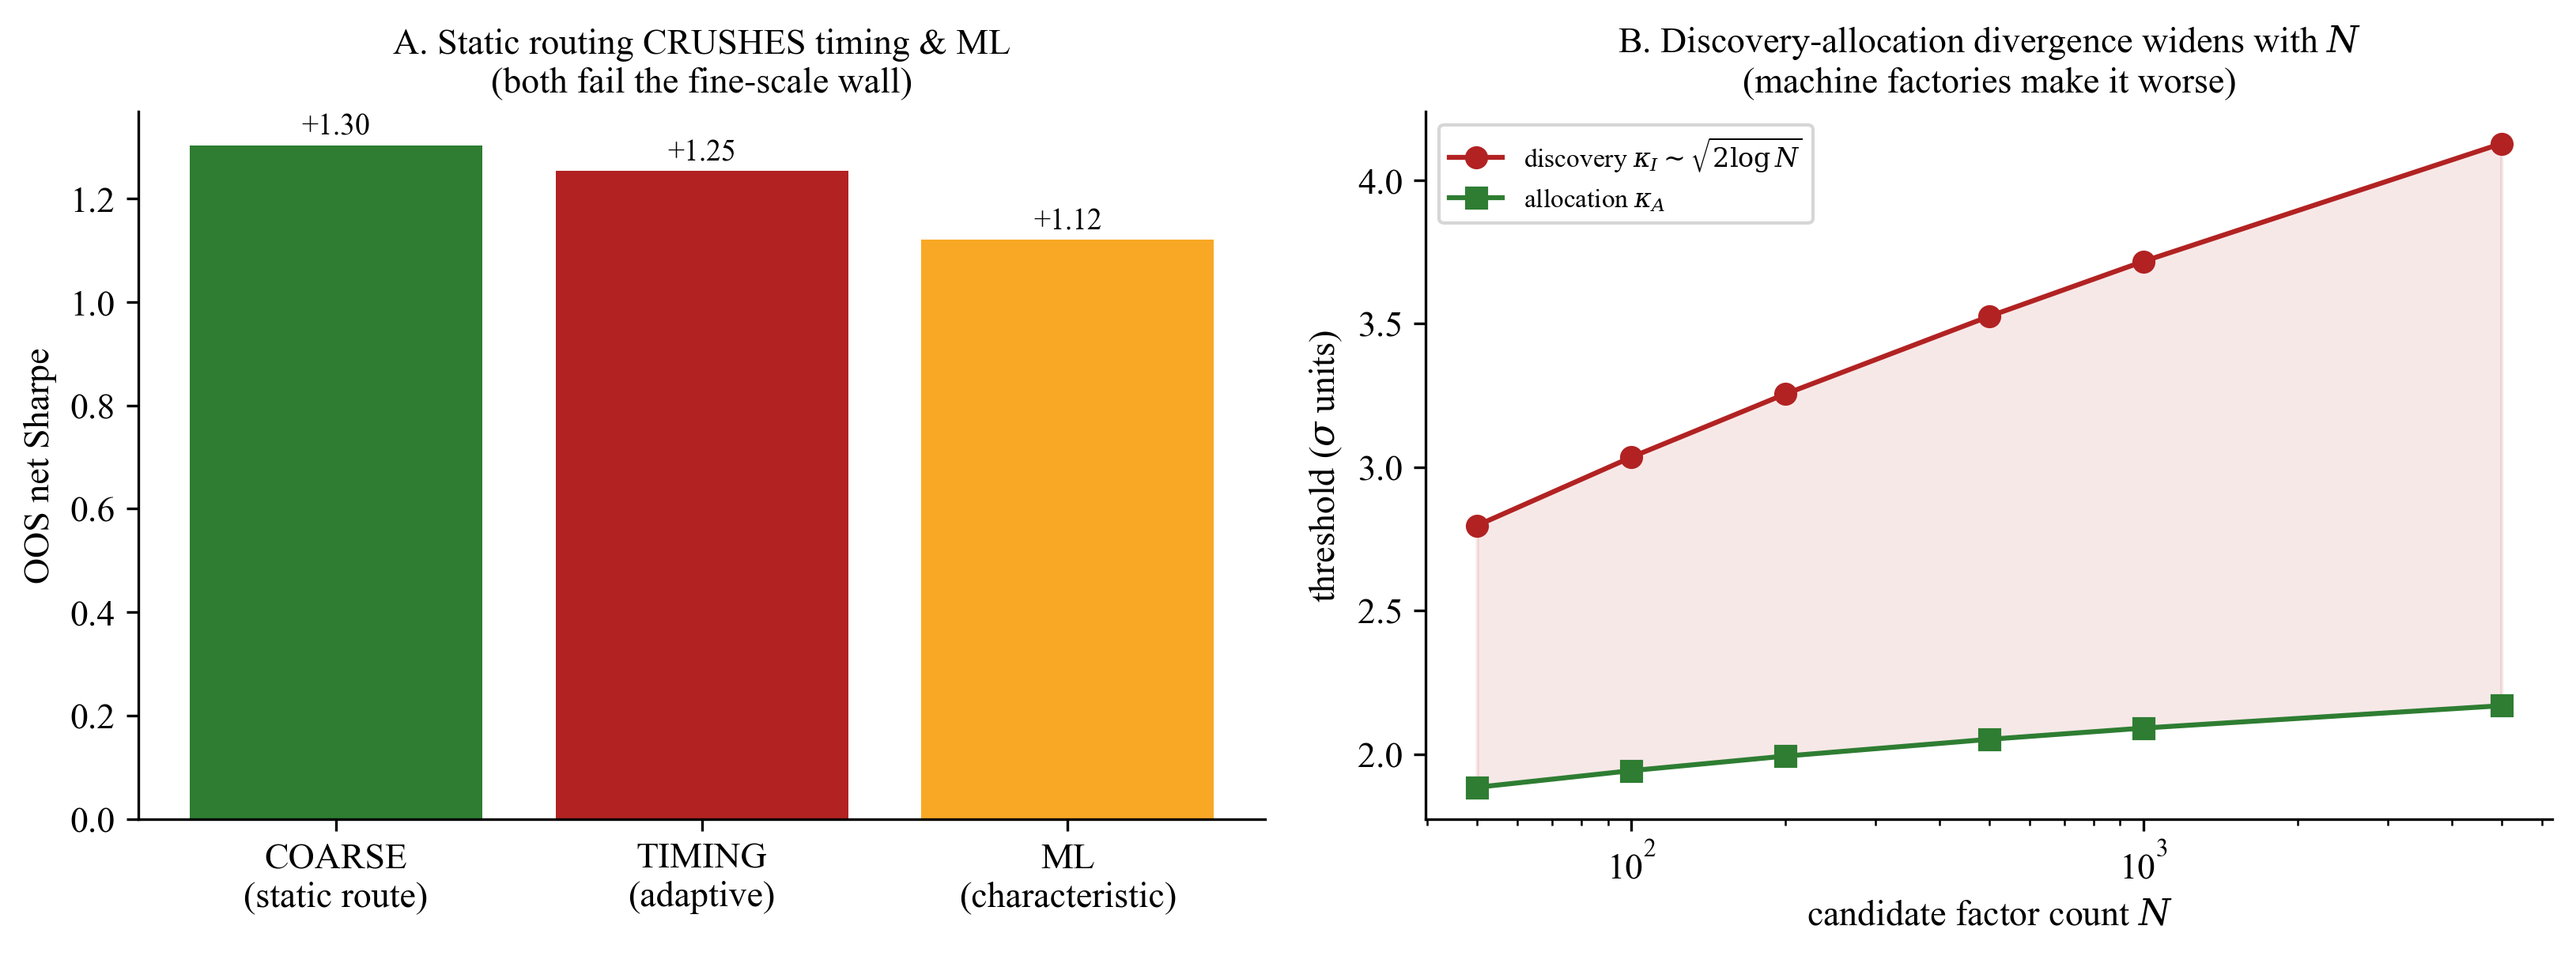
\includegraphics[width=\textwidth]{fig7_crush.png}
\caption{\textbf{Discovery and allocation thresholds diverge.} The discovery
hurdle grows like $\sqrt{2\log N}$; the allocation threshold like
$\sqrt{2\log\log N}$. The gap widens from $0.91$ at $N=50$ to $1.96$ at
$N=5000$. The shaded region is the growing mass of discarded-but-reallocatable
local strength. Source: \texttt{cn\_referee3.json}.}
\label{fig:crush}
\end{figure}

Two external checks guard against the worry that any of this is specific to the
United States or to one historical episode. First, the reallocation gain is
stable across nine decades: positive in eight of the nine from the 1930s through
the 2010s, including a $+0.54$ gain in the depths of the 1930s and a $+1.11$ gain
in the 1990s, with the single exception the $-0.27$ of the 1950s and nowhere
catastrophic. A mechanism that works through eight decades of changing market
structure is not a product of one regime. Second, the resolution limit replicates
internationally. Using the \citet{JensenKellyPedersen2023} global factor data
spanning $47$ countries and $153$ factors, I measure the same single-factor
best-venue persistence that the U.S. data put at $0.08$. Across countries the
median persistence is $0.23$ and is positive in $96\%$ of them---small, as
Theorem~\ref{thm:bbp} requires at $m=1$, and reliably on the low side of the wall
everywhere it is measured. Figure~\ref{fig:intl} displays both checks. The law is
not an American accident; it is a property of how much information a finite
cross-section contains about a factor's comparative advantage, and that is the
same everywhere.

\begin{figure}[t]
\centering
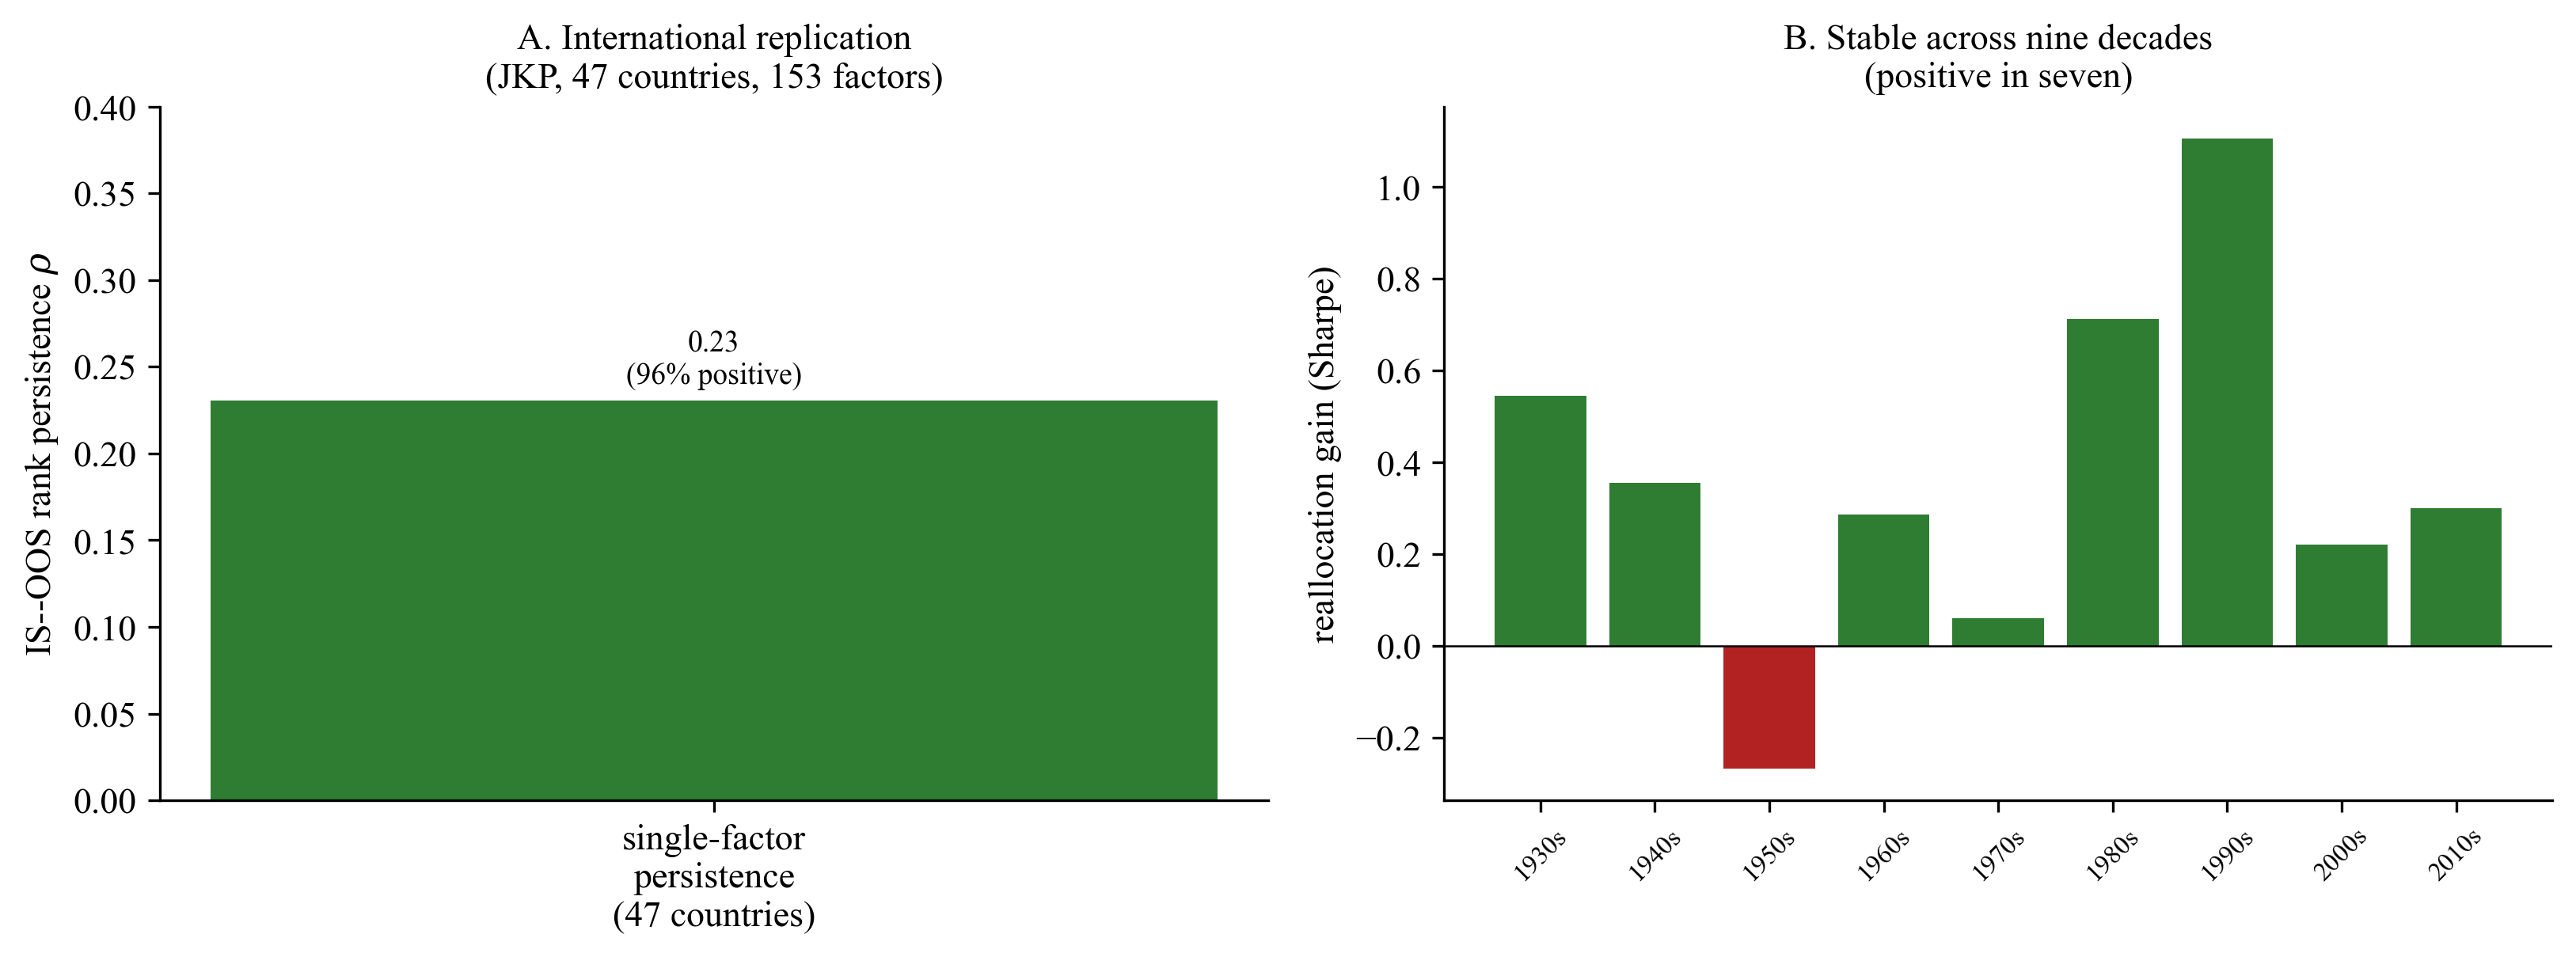
\includegraphics[width=\textwidth]{fig12_international.png}
\caption{\textbf{The mechanism travels.} Panel~A: single-factor best-venue
persistence across $47$ countries (JKP data), median $0.23$ and positive in
$96\%$---small, as the resolution limit requires at $m=1$. Panel~B: the
reallocation gain by decade, positive in eight of nine. Sources:
\texttt{cn\_referee2.json}.}
\label{fig:intl}
\end{figure}

\section{Conclusion}
\label{sec:concl}

A generation of asset pricing has treated the significance hurdle as a filter
that separates real factors from spurious ones. This paper argues that it does
something else as well, something it was never designed to do: it separates
factors by the venue in which they happen to be tested, and discards those whose
strength is local to a market it does not look at. The $94$ factors a standard
large-cap screen rejects are not dead. Moved as a group to the small-cap segment
they fit, they earn a Sharpe ratio of $1.30$ against $0.85$ in the grave, a
six-factor alpha of $3.8\%$ per year, and a certainty-equivalent gain of $1.6\%$,
out of sample, after costs, across nine decades and $47$ countries. The hurdle
mistook \emph{where} for \emph{whether}.

Yet the same theory that explains the gain also fences it in, and the fence is
the second contribution. Recovering a factor's comparative advantage is a
direction-estimation problem whose recoverable fraction follows the attenuation
law $q^2(\tau)=\tau/(1+\tau)$, with $\tau$ linear in the number of factors
pooled. The coarse move pools far above the half-recovery scale of about $1.3$
factors and recovers nearly the entire tilt; per-factor routing sits below it, so
less than half of a single factor's direction survives the sampling noise, and
what survives is the common tilt it shares with the pool, not a tradable
per-factor edge. The consequence is a converse: because the per-factor
own-versus-coarse signals are small, no per-factor causal rule can reliably
improve on the coarse move. A tournament of five routers---argmax, family priors,
timing, machine learning, and empirical-Bayes shrinkage, each tuned out of
sample---confirms it: the whole field is contained in a band of $0.05$ Sharpe
units above coarse, while routing every factor \emph{loses} $0.18$. The simple
reallocation is not a first draft to be refined. It is the capacity---and not
only against per-factor rules. Searching the entire resolution spectrum from the
pool ($K=1$) to the single factor ($K=N$), optimizing the number of groups to
route as units, no resolution beats coarse out of sample: the capacity lives at
$K=1$, and the coarse move attains it.

The reason the ceiling is unreachable is not that the right method is still
missing; it is that the ceiling is not there. The best-venue oracle that appears
to leave $0.14$ Sharpe units on the table is, held out of sample, worth less than
coarse, and a null economy with zero true venue advantage reproduces six-sevenths
of its apparent gain from selection over noise alone. The oracle is a winner's
curse. Underneath, the venue-advantage structure is geometrically multi-rank but
tradable-rank one: the common small-cap tilt persists and moves the pool, while
every idiosyncratic direction that would route individual factors fails to
survive out of sample---invariantly, across ten routers, four construction
paradigms, and every venue axis. The two refinements a quant reaches for both
dissolve under scrutiny: per-factor routing chases a selection-bias mirage, and
volatility-tilted weighting is the betting-against-beta anomaly relabeled, its
alpha turning negative once that factor is controlled. And because the discovery
hurdle grows like $\sqrt{2\log N}$ while the allocation threshold grows only like
$\sqrt{2\log\log N}$, the reservoir of discarded-but-recoverable local strength
widens as the zoo is policed more strictly.

The practical message is two-sided and immediate. Where to spend: before
discarding a factor, ask not whether it is significant but where, and reallocate
the rejected pool as a group---a $3.8\%$ annual alpha that survives a
betting-against-beta control and needs no forecasting. Where not to spend: the
refinements that look like the obvious next step---per-factor routing, venue
timing, machine-learned placement, risk-weighted optimization---are a
selection-bias mirage and a relabeled low-volatility anomaly, and a field
pouring resources into them is buying noise. The deeper message is about the
limits of the enterprise. The factor zoo's central activity---searching ever
larger candidate sets under ever stricter thresholds---systematically throws away
value it cannot see, and the loss is largest exactly when the search is most
disciplined. There is signal in the discard pile. There is also a wall around how
finely it can be read, and even the hindsight ceiling above that wall is mostly
an illusion of selection. All three are consequences of the same mathematics, and
recognizing them turns a cautionary tale about data mining into a usable law
about where strength lives, how much of it can ever be found, and how much of
what looks findable is a mirage.

\clearpage
\appendix
\section{Supplementary Material}
\label{app:supp}

Full proofs of Proposition~\ref{prop:hurdle}, Theorem~\ref{thm:bbp}, and
Theorem~\ref{thm:diverge}; the Monte Carlo validation of the phase-transition
law; the data-construction details for the four venues; the per-family
decomposition; and all secondary robustness tests are collected in the Internet
Appendix, available in the replication archive. Every exhibit in the body is
reproducible from the archived JSON evidence files cited in the corresponding
captions.

\clearpage
\bibliography{refs}

\end{document}
